\def\FORMAT{}
\documentclass[11pt]{book}
\usepackage{amsmath,mathtools}
\usepackage[utf8]{inputenc}
\usepackage[ngerman]{babel}
\usepackage[T1]{fontenc}
\usepackage{lmodern}
\usepackage{acronym}
\usepackage{graphicx} 
\usepackage{epstopdf}
\usepackage{svg}
\usepackage{multirow}
\usepackage{amssymb}
\usepackage{trfsigns}
\usepackage{setspace}
\usepackage{yfonts}
\usepackage{nomencl}
\usepackage{float}
\usepackage{subfig}
\usepackage{scrpage2}
\usepackage{afterpage}
\usepackage{longtable}
\usepackage[author={Michael Meindl}]{pdfcomment}

\onehalfspacing


%Hyperlinks package, links aus inhaltsverzeichnis
\usepackage{hyperref}
\hypersetup{
    colorlinks=false, %set true if you want colored links
    linktoc=all,
    linkbordercolor = {white},
    citecolor = {white},
    allbordercolors = {white},
}
%Blattformatierung
\usepackage{geometry}
\geometry{a4paper, top=25mm, left=30mm, right=25mm, bottom=20mm}

%Listing
\usepackage{courier}
\usepackage{listings}
\usepackage{color}
 \lstset{
   frame=tb,
   framexleftmargin=2.5em,
   basicstyle=\small\linespread{0.9}\bfseries\ttfamily,
   emph={square}, 
   emphstyle=\color{blue}\texttt,
   emph={[2]root,base},
   emphstyle={[2]\color{yac}\texttt},
   showstringspaces=false,
   flexiblecolumns=false,
   tabsize=2,
   numbers=left,
   numberstyle=\small\bfseries\ttfamily,
   numberblanklines=false,
   stepnumber=1,
   numbersep=10pt,
   xleftmargin=25pt
 }
 
 \def\presuper#1#2%
	{\mathop{}%
	\mathopen{\vphantom{#2}}^{#1}%
	\kern-\scriptspace%
	#2}
%Display vecotr in a reference frame
\newcommand{\vecBS}[4]{\presuper{#1}{\begin{pmatrix}
#2 \\ #3 \\ #4
\end{pmatrix}}}
%Boldsymbol shortcut
\newcommand{\bs}[1]{\boldsymbol{#1}}
%Bezugssystemdefinition
\newcommand{\defBS}[1]{\{#1\} [ \bs{e}_{{#1}_1},\bs{e}_{{#1}_2}, \bs{e}_{{#1}_3} ]}
%Projektionsmatrix
\newcommand{\pMat}[2]{\presuper{#1}{\bs{P}}^{#2}}
%Differenation in Respekt zu BS
\newcommand{\diffIn}[3]{\frac{\presuper{#1}{d{#2}}}{d#3}}
\newcommand{\partialDiffIn}[3]{\frac{\presuper{#1}{\partial{#2}}}{\partial #3}}
%Geschwindigkeit/Beschleunigung
\newcommand{\vel}[3]{\presuper{#1}{\bs{#2}}^{#3}}

%Rightarrow with spaceing
\newcommand{\rArrow}{\hspace{5pt}\rightarrow\hspace{5pt}}
%Inneres Produkt
\newcommand{\inProd}[2]{\langle {#1}, {#2} \rangle}

%System macro
\newcommand{\cSS}[3]{\textfrak{S}($\bs{#1}$,$\bs{#2}$,$\bs{#3}$)}
\newcommand{\dSS}[3]{\textfrak{D}($\bs{#1}$,$\bs{#2}$,$\bs{#3}$)}

%Laplace transform sign with spaces
\newcommand{\myLaplace}{\hspace{15pt}\laplace\hspace{15pt}}

\newcommand*{\signed}[1]{%
        \nolinebreak[3]\hspace*{\fill}\mbox{\emph{#1}}
    }
%Vektor norm
\newcommand{\norm}[1]{\left\lVert#1\right\rVert}
%Kreuzproduktmatrix
\newcommand{\kProdMat}[1]{\left[ #1 \right]_\times}

%Nicht kursiver Subskript
\newcommand{\idx}[1]{_{\text{#1}}}

%Vertikales Transformationszeichen
\newcommand{\vlaplace}[1][]{\mbox{\setlength{\unitlength}{0.1em}%
                            \begin{picture}(10,20)%
                              \put(3,2){\circle*{4}}%
                              \put(3,4){\line(0,1){12}}%
                              \put(3,18){\circle{4}}%
                              \put(10,7){#1}
                            \end{picture}%
                           }%
                     }%
                     
%Bedingte Wahrscheinlichkeit
\newcommand{\condP}[2]{p({#1} \hspace{1mm} \vert \hspace{1mm} {#2})}

%Cusotm log
\newcommand{\myLog}[1]{\text{log}\left[ {#1} \right]}
\newcommand{\mLog}[1]{\myLog{#1}}
%Custom sin
\newcommand{\mySin}[1]{\text{sin}\left[ {#1} \right]}
\newcommand{\mSin}[1]{\mySin{#1}}
%Custom cos
\newcommand{\myCos}[1]{\text{cos}\left[ {#1} \right]}
\newcommand{\mCos}[1]{\myCos{#1}}
%Custom atan
\newcommand{\myAtan}[1]{\text{atan}\left[ {#1} \right]}
\newcommand{\mAtan}[1]{\myAtan{#1}}

%Custom Matrix-Format
\newcommand{\mat}[1]{\mathbf{\underline{{#1}}}}
%Custom Vector-Format
\newcommand{\mVec}[1]{\vec{\mathbf{#1}}}
\newcommand{\myVec}[1]{\mVec{#1}}

\makeatletter
\def\input@path{{0_Introduction/}{1_Infrastruktur/}{2_GlobalPlaner/}{3_StochastischeModelle/}{4_Kartographierung/}{6_LocalPlaner/}{7_ROSImplementierung/}{8_Lokalisierung/}{9_Ausblick/}{10_Experimente/}}
\makeatother
\graphicspath{{0_Introduction/}{1_Infrastruktur/}{2_GlobalPlaner/}{3_StochastischeModelle/}{4_Kartographierung/}{6_LocalPlaner/}{7_ROSImplementierung/}{8_Lokalisierung/}{9_Ausblick/}{10_Experimente/}}


%-----------------------------------------------------------------
% Beschriftung des Titelblatts - Vorderseite
%-------------------------------------------------------------------

\renewcommand{\maketitle}{
    \begin{titlepage}

    \thispagestyle{empty}

        \oddsidemargin4mm   % Hier BCOR  eingeben  !! 14
        \evensidemargin4mm  %

  \vspace*{10mm}

\begin{center}
  \vspace*{-30mm} % -30 wenn Zeilenabstand 1.2
  \sffamily %\large 
  
%  Hochschule Karlsruhe - Technik und Wirtschaft   \\
  %Fakultät für Maschinenbau und Mechatronik\\
  \vspace{20mm}%
\end{center}

\begin{center}
  \sffamily
  {\huge Hochschule Karlsruhe - Technik und Wirtschaft}
  \vspace*{0.3cm}
  
  {\huge Fakultät für Maschinenbau und Mechatronik}
  \vspace*{2.5cm}
  
   {\huge  \bfseries Autonome Navigation mehrerer TurtleBots im Schwarm \\}
%
    \vspace*{2cm}
%    
    {\huge Forschungs- und Entwicklungsprojekt I}
    \vspace*{2cm}

    {\huge Michael Meindl}
    \vspace*{4cm}
    
    {\huge Betreuer: Prof. Dr.-Ing. Joachim Wietzke}
    \vspace*{2cm}
    
    
    {\Large Karlsruhe, Wintersemester 2017/2018}
    

%
\end{center}
\end{titlepage}
}

\begin{document}
\frontmatter
\pagestyle{scrheadings}
\clearscrheadfoot
\setheadsepline{0pt}
\setfootsepline{0pt}
\maketitle
\afterpage{\null\newpage}

\ohead{\pagemark}
\tableofcontents
\listoffigures\addcontentsline{toc}{chapter}{Abbildungsverzeichnis}
\lstlistoflistings\addcontentsline{toc}{chapter}{Listings}
%%==============================================================
%
% Nomenklatur
%
%==============================================================
\chapter*{Nomenklatur}
  \label{Nomenklatur}%
   % Die folgende Zeile erzwingt einen Eintag ins Inhaltsverz.
  \addcontentsline{toc}{chapter}{Nomenklatur}%
%-----------
\manualmark
\markright{Nomenklatur}
\markleft{Nomenklatur}
%\ohead[]{\headmark}
\begin{longtable}{p{0.15\textwidth} p{0.75\textwidth}}  % ACHTUNG Breite 0.9
%-----------------------------------------------
\multicolumn{2}{l}{%
\textbf{\textsf{\large Schreibeweise mathematischer Symbole}}
}\\
$\bs{a}$ & Vektor wird fett und klein geschrieben \\
$\bs{a}^T$ & Transponierter von Vektor $\bs{a}$ \\
$\bs{A}$ & Matrix wird fett und groß geschrieben \\
$\bs{A}^T$ & Transponierte der Matrix $\bs{A}$ \\
$\inProd{\bs{a}}{\bs{b}}$ & Skalarprodukt der Vektoren $\bs{a}$ und $\bs{b}$ \\
$\kProdMat{\bs{b}}$ & Kreuzproduktmatrix des Vektors $\bs{b}$ ($\bs{b}\times \bs{a}$ = $\kProdMat{\bs{b}}\cdot \bs{a})$ \\
$s_{\varphi}$ &	 Sinus des Winkels $\varphi$ \\
$c_{\varphi}$ &  Cosinus des Winkels $\varphi$ \\
\\
\multicolumn{2}{l}{%
\textbf{\textsf{\large Symbole der technischen Mechanik}}
}\\
$\presuper{A}{\bs{b}}$ & Vektor $\bs{b}$ aus Perspektive des Bezugssystem $A$ \\
$\vel{A}{v}{B}$ & Geschwindigkeit von $B$ relativ zu $A$ \\
$\vel{A}{a}{B}$ & Beschleunigung von $B$ relativ zu $A$ \\
$\vel{A}{\omega}{B}$ & Winkelgeschwindigkeit von $B$ relativ zu $A$ \\
$\vel{A}{\alpha}{B}$ & Winkelbeschleunigung von $B$ relativ zu $A$ \\\
$q$ & Generalisierte Koordinate \\
$u$ & Generalisierte Geschwindigkeit \\
$\vel{A}{v}{B}_i$ & Partielle Geschwindigkeit $i$ von $B$ relativ zu $A$ \\
$\vel{A}{\omega}{B}_i$ & Partielle Winkelgeschwindigkeit $i$ von $B$ relativ zu $A$ \\
$F$ & Generalisierte aktive Kraft \\
$F^*$ & Generalisierte Trägheitskraft \\
$\bs{T}^{A/B}$ & Auf $A$ wirkendes Drehmoment mit dem Drehpunkt $B$ \\
$\bs{T}^{A/B}_*$ & Auf $A$ wirkendes Trägheitsmoment mit dem Drehpunkt $B$ \\
$I$ & Trägheitsskalar bzw. Massenträgheitsmoment \\
$\bs{I}$ & Trägheitstensor \\
\newpage
\multicolumn{2}{l}{%
\textbf{\textsf{\large Symbole der Regelungstechnik}}
}\\
\textfrak{S} & Zeitkontinuierliches System \\
\textfrak{D} & Zeitdiskretes System \\
$\bs{x}$	 & Zustandsvektor \\
$\bs{u}$	 & Eingangsvektor \\
$\bs{y}$     & Ausgangsvektor \\
$\bs{A}$     & Systemmatrix \\
$\bs{B}$	 & Eingangsmatrix \\
$\bs{C}$	 & Ausgangsmatrix \\
$\bs{K}$	 & Reglermatrix \\
$\bs{L}$	 & Beobachtermatrix \\
$\bs{0}^{i\times j}$ & Nullmatrix des Raumes $\mathbb{R}^{i\times j}$ \\
$\bs{I}^{i\times i}$ & Einheitsmatrix des Raumes $\mathbb{R}^{i\times i}$ \\
\\
\multicolumn{2}{l}{%
\textbf{\textsf{\large Abkürzungsverzeichnis}}
}\\
SISO 		& Single-Input-Single-Output \\
MIMO		& Multiple-Input-Multiple-Output \\
SPI			& Serial Peripheral Interface \\
CS			& Chip-Select \\
ADC			& Analog-to-Digital Converter \\
GPIO		& General Purpose Input/Output \\
BBB			& BeagleBone Black \\
FSM			& Finite-State-Machine \\
LQR			& Linear-Quadratische Regelung \\


\end{longtable}

\cleardoublepage






















\mainmatter
\pagestyle{scrheadings}
\clearscrheadfoot
\setfootsepline{1pt}
\setheadsepline{1pt}
\ohead{\pagemark}
\ihead{\headmark}
\automark[section]{chapter}

\chapter{Einleitung}
\pdfcomment{Herleitung Aufgabe/Chor-Geschichten}Seit einiger Zeit wird an der Hochschule Karlsruhe die Projektidee eines künstlichen Chors verfolgt, dessen Ziel darin besteht, eine Audiospur simultan in mehreren Tonhöhen wiederzugeben, um einen mehrstimmigen Chor zu erzeugen. Das zugrundeliegende technische Prinzip lässt sich recht leicht erläutern: die originale Tonspur wird mittels FFT in den Frequenzbereich transformiert, wo das Signal in die gewünschte Tonhöhe bzw. Frequenzbereich verschoben wird. Anschließend werden die Signale zurück in den Zeitbereich transformiert und abgespielt. Allerdings gestaltet sich die Umsetzung weitaus anspruchsvoller als das theoretische Konzept. Beispielsweise führen Aussetzer im WLA-Netzwerk, Puffergrößen der Audiotreiber und diskrete Stützstellen des Frequenzspektrums zu unerwarteten Problemen, die sich in Form von knackenden Lautsprechern Gehör verschaffen. Nichtsdestotrotz hat der Entwicklungsprozess den Punkt erreicht, an dem der Chor noch kaum unerwünschte Töne von sich gibt, weshalb nun die erste große Erweiterung angestrebt wird. Aktuell setzt sich das System aus einem Master-PC und vier BeagleBones zusammen, die jeweils mit einem Lautsprecher ausgestattet in einem Raum verteilt werden. Auf dem Master wird eine Tonspur eingespielt, die er in die gewünschten Tonhöhen pitcht und per WLAN an die BeagleBones sendet, welche jeweils eine der Stimmen über den Lautsprecher wiedergeben.
\par
\pdfcomment{Ziel von fahrendem Roboter}Im nächsten Schritt soll der Chor mobilisiert werden. Das heißt jedes BeagleBone plus Lautsprecher wird auf einem Roboter montiert, die bei einer Vorführung einen beliebigen Raum betreten können und diesen auf der Suche nach einem passenden Podium erkunden. Wurde Letzteres gefunden, so sollen sich die Roboter dort im Halbkreis formieren und anschließend vorsingen.

Die neue Aufgabe, die sich mit der autonomen Navigation der Roboter beschäftigt, kann vollkommen entkoppelt von dem Chor betrachtet und bearbeitet werden. Dieser zweite Entwicklungsstrang befindet sich allerdings noch im Anfangsstadium, da sich bisher nur ein einzelnes Entwicklungsprojekt \cite{Turtleboys} dem Thema gewidmet hat. In dieser Arbeit wurde ein erster Grundstein gelegt, der sich einerseits aus der Auswahl und Inbetriebnahme der Roboter, andererseits aus einem ersten Proof-of-Concept in Sachen Navigation zusammensetzt.

\pdfcomment{Turtlebot als Hardware}Als mobile Plattform für die Lautsprecher fiel die Wahl auf den Turtlebot 2 \cite{Turtlebot}, der von Willow Garage entwickelt wurde. Der Roboter setzt sich aus der Kobuki-Basis, einem Rechner und einer ASUS-Xtion-Pro-Live zusammen, wobei Letztere sowohl Kamera als auch Tiefensensor zur Verfügung stellt. Der Turtlebot 2 bringt als Vorteil mit sich, dass der Roboter weite Anwendung im Bereich von Hobby- und Forschungsanwendungen findet, weshalb eine breite Community-Untersützung zur Verfügung steht. Ein in dieser Arbeit wichtiges Beispiel stellt die Simulation des Roboters mithilfe von GAZEBO \cite{gazebo} dar: Hier besteht bereits eine vollständige Integration des Turtlebot 2, die quelloffen zugänglich ist. Im Rahmen der Vorgängerarbeit wurde der Roboter zusätzlich mit dem Laserscanner Tim551 der Marke SICK ausgestattet \cite{SICK}, der als primärer Sensor für die Navigation verwendet wird.

\pdfcomment{Robot-Operating-System}Die Programmierung erfolgt mithilfe des sogenannten Robot-Operating-System (ROS), wobei es sich ironischerweise um kein Betriebssystem sondern eine Middleware handelt, die eine Vielzahl von Tools und Paketen für die autonome Navigation bereitstellt. Dadurch müssen die Algorithmen für die Navigation und Kartographierung nicht eigenständig implementiert werden, sondern können in Form von ROS-Paketen eingesetzt werden, sodass sich die Inbetriebnahme auf die Parametrisierung der ROS-Funktionen beschränkt. Außerdem beinhaltet ROS ein Netzwerk, über das die Roboter kommunizieren können. Mithilfe der Kommunikationskanäle können auch externe Werkzeuge auf relevanten Daten zugreifen, womit komfortable und effiziente Debugging-Wege geschaffen werden. Umgekehrt können zu Beginn die Roboter auch aus dem Netz entfernt und durch ein Simulationstool wie GAZEBO ersetzt werden. So können die Algorithmen zunächst anhand einer Simulation erprobt und konfiguriert werden und im Anschluss unverändert auf die Roboter übertragen werden.

\pdfcomment{Erste Navigation mittels Navigation-Stack}Die im Vorgängerprojekt \cite{Turtleboys} erarbeitete Navigationslösung basiert auf dem ROS-Navigation-Stack und setzt sich aus zwei Teilen zusammen. Im ersten Schritt wird mit dem ROS-Paket \lstinline{hector_slam}{} \cite{WikiHector} eine Karte der Umgebung aufgezeichnet. Anschließend navigieren die Roboter anhand der Karte zu dem vorgegebenen Ziel, wobei das ROS-Paket \lstinline{move_base}{} \cite{WikiMoveBase} zum Einsatz kommt. Bei dessen Konfiguration wurden zwei verschiedene Ansätze verfolgt: Bei dem Ersten erfolgt die Lokalisierung des Roboters ausschließlich anhand der Odometriedaten. Der zweite Ansatz greift auf die AMC-Lokalisierung zurück. Der Vorteil der zweiten Variante liegt darin, dass die Ausgangsposition des Roboters nicht bekannt sein muss. Bei der Navigation mittels Odometrie übertragen sich sämtliche Fehler bei der Angabe der Anfangsposition unmittelbar auf die Navigation. Im Gegensatz dazu verspricht die AMCL-Variante - zumindest theoretisch - ein höheres Maß an Robustheit. Allerdings konnte diese Hoffnung in den Experimenten nicht bestätigt werden, weshalb letzten Endes die Odometrie-Navigation verwendet wurde \cite[S. 43]{Turtleboys}. Zusätzlich sei angemerkt, dass diese Lösung nicht im Stande ist, Hindernisse, die nicht auf der Karte verzeichnet sind, während der Navigation zu erkennen, geschweige denn, denen auszuweichen.

\pdfcomment{Funktionale Anforderungen}An dieser Stelle knüpft die vorliegende Arbeit an: Die Navigation soll an den Punkt gebracht werden, wo die Roboter im Stande sind, sich selbst auf der Karte zu lokalisieren, unerwartete Hindernisse zu detektieren und diesen entsprechend auszuweichen. Hierfür soll auf bestehende Möglichkeiten des ROS-Navigation-Stack zurückgegriffen werden, um die Menge von Lösungsmöglichkeiten einzuschränken. Auch die Anforderung, dass die Navigation auf eine mit \lstinline{hector_slam}{} aufgezeichnete Karte zurückgreifen kann, wird übernommen. Im ersten Schritt wird lediglich ein einzelner Roboter betrachtet. Sobald dieser die Anforderungen im Bereich der autonomen Navigation erfüllt, werden die Ergebnisse auf eine Gruppe von vier Robotern übertragen.

Die funktionalen Anforderungen dieser Arbeit bestehen darin, die autonome Navigation mehrerer Roboter zu ermöglichen. Darüber hinaus besteht der Anspruch darauf, die zugrundeliegenden Algorithmen nachzuvollziehen und zu verstehen. Die ROS-Implemententierung sollen nicht nur derartig parametrisiert werden, damit die funktionalen Anforderungen erfüllt sind. Sondern es soll der Zusammenhang zwischen den Parametern und dem Funktionsprinzip der Navigation erarbeitet werden, sodass Letzteres verstanden werden kann. Hierfür werden zu Beginn der Arbeit theoretische Grundlagen der Planung und stochastischen Modellierung diskutiert, deren elaborierte Ausführungen die Bausteine der autonomen Navigation bilden.
Ein Hauptproblem der Navigationsaufgabe besteht darin, dass die Teilprobleme nicht entkoppelt betrachtet werden können, woraus eine unerwünschte Komplexität resultiert. Um die einzelnen Komponenten isoliert betrachten zu können, wird im Rahmen dieser Arbeit auf Simulationswerkzeuge wie MATLAB und GAZEBO zurückgegriffen, in denen Daten, die unter realen Umständen mittels zusätzlicher Algorithmen geschätzt werden müssen, unmittelbar abgegriffen werden können. Anhand dieser vereinfachten Beispiele erfolgt die Diskussion der Teilprobleme wie Planung und Lokalisierung. Im Anschluss wird auf die ROS-Implementierung der Algorithmen eingegangen, die zuletzt in Betrieb genommen und in reellen Szenarien getestet wird.

Zu Beginn der Arbeit wird ROS' Navigation-Stack in seine einzelnen Komponenten unterteilt und deren Hauptfunktionen beschreiben. Im Anschluss wird das Funktionsprinzip der einzelnen Komponenten im Detail betrachtet. Diese Untersuchung beginnt bei dem globalen Planer, der als einzige Komponente mit deterministischen Modellen arbeitet und deshalb eine Sonderstellung unter den Komponenten einnimmt. Die restlichen Komponente basieren auf stochastischen Modellen, weshalb im Anschluss zuerst die Bedeutung von stochastischen Modellen in der Robotik diskutiert und am Beispiel eines Bewegungs- sowie Messmodells erläutert wird.

Der darauffolgende Abschnitt widmet sich der Kartenerstellung, wobei es sich um ein Aufgabe handelt, die nicht Teil des Navigation-Stacks ist. Allerdings bietet der hier verwendete Kartographierungsalgorithmus einen Einblick in das Funktionsprinzip stochastischer Modelle und rundet das Verständnis der Navigation insofern ab, dass nach wie vor Karten hierfür erforderlich sind. Als letzter Teil des Navigationstack wird der lokale Planer diskutiert, der auf den Dynamic Window Approach zurückgreift, um die Steuerbefehle des Roboters zu berechnen.
Ein weiterer wichtiger Aspekt für die Navigation stellt die Lokalisierung dar, weshalb im Anschluss die adaptive Monte-Carlo-Lokalisierung (AMCL) diskutiert wird, die auch unter ROS zum Einsatz kommt. 

Der Funktionsnachweis der Navigation erfolgt anhand von drei Experimenten. Zunächst wird der Fall betrachtet, dass der Roboter in dem im Vergleich zur Kartenerstellung unveränderten Raum navigieren müssen. Hierbei wird die Grundfunktion der Navigation bewiesen. Im folgenden Experiment wird der Weg des Roboters durch ein unbekanntes Hindernis versperrt, weshalb Sensordaten in die Pfadplannung integriert werden müssen, um das Objekt zu detektieren und bei der Planung zu beachten. Im letzten Versuch wird die Lokalisierung des Roboters untersucht, wofür dieser an einer unbekannten Position ausgesetzt wird, die nur durch eine ungenaue Schätzung vorgegeben wird. Hieran wird ersichtlich wie der Roboter sich orten kann, wenn er eine kurze Distanz zurücklegt, um neue Information über seine Umgebung zu sammeln.

Zuletzt wird die Implementierung der Navigationskonzepte unter ROS betrachtet. Hier werden die verschiedenen Launch-Dateien zur Fernsteuerung, Kartenaufzeichnung und Navigation vorgestellt. Außerdem wird das Zusammenspiel des Master- und der Slave-PCs beschrieben.

\chapter{Aufbau des Gesamtsystem und Infrastruktur}
\pdfcomment{Wofür?}In der Endvorstellung des Projektes navigieren vier Roboter simultan durch denselben Raum, woran recht leicht ersichtlich wird, dass ein Weg zum Datenaustausch zwischen den Robotern geschaffen werden muss. Auch eine zentrale Steuereinheit soll in der Lage sein, alle Roboter anzusprechen und zu dirigieren. Selbst ein einzelner Roboter stellt bereits einige Anforderungen an die Kommunikationsstruktur: Da eine erfolgreiche Navigation auf dem Zusammenspiel mehrerer komplexer Algorithmen basiert, müssen externe Analysetools relevante Daten abgreifen, die zwischen den Komponenten ausgetauscht werden. Diese Form des Debuggings ist unerlässlich, um das Verhalten des Roboters nachvollziehen zu können. In diesem Projekt erfüllt ROS diese Anforderungen, weshalb in den folgenden Abschnitten das Kommunikationskonzept unter ROS erläutert wird. Auch die Simulations- und Analysewerkzeuge, die in der Arbeit zum Einsatz kommen, werden vorgestellt und deren ROS-Schnittstellen erläutert.

\pdfcomment{ROS-Netzwerk}Jeder TurtleBot ist mit einem Mini-PC ausgestattet, auf denen Ubuntu 14.04 und ROS-Indigo installiert sind. Als zentrale Steuereinheit des Roboterverbundes fungiert ein weiterer Mini-PC, der über WLA-Netzwerk mit den Roboter-PCs verbunden ist. Das private Netzwerk wird mittels eines TP-Link Routers verwaltet, in dem auch weitere Entwicklungsrechner beitreten können. Auf dem Master-PC wird \lstinline{ros_core}{} ausgeführt, über den die Kommunikation abläuft. Als Kommunikationsmittel werden in ROS Nachrichten verwendet, die jeweils unter einer so genannten \lstinline{topic}{} veröffentlicht werden. Beispielsweise versendet der Laserscanner zyklisch eine Nachricht des Typs \lstinline{sensor_msg/laser_scan}{} unter der topic \lstinline{/scan}{}. Alle Nodes, die an den Sensordaten interessiert sind, abonnieren die Topic. Indem Analysewerkzeuge wie MATLAB relevante Topics mithören, können die zugehörigen Daten aufgezeichnet und visualisiert werden. Umgekehrt ist es auch möglich den TurtleBot vollständig durch eine Simulation zu ersetzen. Gazebo veröffentlicht alle Topics, die für gewöhnlich von dem TurtleBot versendet werden, wodurch dieser ersetzt wird. Die restlichen Bestandteile des Netzwerkes bleiben erhalten, weshalb der Wechsel zwischen Realität und Simulation mühelos abläuft.

\pdfcomment{Simulationswerkzeug: Gazebo} Die Idee Gazebo in Verbindung mit ROS für die Simulation zu verwenden entstammt der Arbiet \cite{ROSGazebo}. Dort wurde unter einer ähnlichen Konfiguration ein P3-DX Roboter verwendet. Der primäre Vorteil dieser Simulationsstruktur besteht darin, dass die Algorithmen und Konfigurationen unverändert von der Simulation auf den Roboter übertragen werden können. Gazebo bietet auch für die TurtelBots eine vollständige Unterstützung, das heißt es besteht eine frei zugängliche Integration des TurtleBot in Gazebo. Allerdings existiert keine Implementation des hier verwendeten Laserscanner, Tim551, weshalb die Sensorik nicht exakt abgebildet werden kann. Prinzipiell können die Sensoren eingepflegt werden, was jedoch im Rahmen dieser Arbeit aus zeitlichen Gründen nicht erfolgt ist. Daraus resultiert der Nachteil, dass die Simulation nur beschränkt Schlüsse auf die Realität zulässt. Nichtsdestotrotz ergeben sich zwei wichtige Vorteile: Einerseits können die verschiedenen Konfigurationen des ROS-Navigation-Stack anhand der Simulation erprobt und auf ihre Richtigkeit überprüft werden, bevor sie auf reale Anwendungsfälle übertragen werden. Andererseits können im Rahmen der Simulation die Komponenten des Navigation-Stack vollkommen entkoppelt werden. Beispielsweise hängen die Ergebnisse der Navigations-Algorithmen stark von der Qualität der Lokalisierung ab, weshalb die Planungs- und Lokalisierungsproblematik in einem realen Umfeld nicht getrennt untersucht werden können. In der Simulation können Positionsdaten jedoch unmittelbar abgegriffen und der Navigation zur Verfügung gestellt werden. Insofern stellt Gazebo ein mächtiges Werkzeug für die schrittweise Inbetriebnahme des Navigation-Stacks dar.

\pdfcomment{Simulationswerkzeug: MATLAB}MATLAB kann im Rahmen der Robotics-Toolbox ebenfalls als ROS-Node betrieben werden, wodurch eine Schnittstelle zwischen MATLAB und ROS geschaffen wird. Hier bringt MATLAB den Vorteil mit sich, dass es für die Implementierung von Algorithmen oftmals besser geeignet ist als C++ oder auch Python. Insbesondere die Möglichkeiten im Bereich der Visualisierung von Karten und Plots erweisen sich als mächtige Werkzeuge bei der Implementierung und Erprobung von Algorithmen. Außerdem können simple Anwendungsszenarien, wie sie zum Beispiel im Rahmen der diskreten Planung auftreten, vollständig mit MATLAB simuliert werden.

\pdfcomment{Visualisierungswerkzeug: RViz}Als letztes Werkzeug sei an dieser Stelle RViz genannt, das als ROS-Paket vorliegt und für die Visualisierung von Robotikanwendungen konzipiert wurde. Mithilfe von RViz können sowohl Karten als auch Roboter und Pfade graphisch dargestellt werden. Da RViz für die Anwendung mit ROS konzipiert wurde, stehen vollständige Konfiguration für den Einsatz mit der autonomen Navigation zur Verfügung, die Out-of-the-Box genutzt werden können.

\chapter{Funktionsprinzip des globalen Planers}
Wie bereits erwähnt, wird die Navigationsaufgabe mithilfe zweier sukzessiver Planungsalgorithmen gelöst. Im ersten Schritt berechnet ein globaler Planer einen Weg zwischen der Ausgangs- und Zielposition, wofür die vorgegebene Karte herangezogen wird. Als Planungsalgorithmus werden im Navigation-Stack entweder Dijkstra- oder der A*-Algorithmus verwendet, die an dieser Stelle näher untersucht werden. Prinzipiell besteht die Aufgabe darin, einen Weg und Trajektorie zu ermitteln, die den Ausgangszustand des Roboters mit dem gewünschten Endzustand verbinden. Bei den gesuchten Pfaden handelt es sich um zeit- und ortskontinuierliche Kurven, woraus ein kontinuierlicher Raum von Lösungen resultiert, der nach einer optimalen durchsucht werden muss. Die Kontinuität des Suchraums stellt auf der Planungsseite eine immense Herausforderung dar, da in diesem Fall Gütefunktionale optimiert werden müssen. Um dieser Komplexität Herr zu werden, wird der Suchraum diskretisiert und die Planungsaufgabe auf die Bestimmung einer Positionsfolge reduziert.

Allerdings wird die Diskretisierung des Raumes von mehr als einer reinen Vereinfachung des Suchproblems motiviert: Der globale Planer übernimmt lediglich den ersten Schritt bei der Berechnung der letztendlichen Trajektorie. Der lokale Planer ermittelt anhand der globalen Sollkurve eine lokale Trajektorie, die in Form von Stellgrößen realisiert wird. Dabei werden neben der globalen Ortskurve auch aktuelle Sensor- und Lokalisierungsinformationen miteinbezogen, welche unter Umständen dazu führen können, dass der Roboter von der global geplanten Kurve abweicht. Insofern ergibt es wenig Sinn, bei der globalen Planung Ressourcen in eine unnötig genaue Trajektorie zu investieren; besonders dann, wenn noch nicht alle nötigen Informationen vorliegen. Für den Anfang genügt ein ungenauer, fehlerbehafteter Pfad, der die Anfangs- und Zielposition verbindet, wofür eine diskrete Darstellung des Suchraums vollkommen genügt. Des Weiteren stimmt die Forderung nach einer diskreten Darstellung des Suchraums mit den üblichen Darstellungsformen von metrischen Karten überein, denn diese repräsentieren die Umgebung in Form von diskreten Zellen.

\pdfcomment{Formulierung}Im Rahmen dieser Überlegung werden die vereinfachten Bedingungen zunächst in einer mathematischen Darstellung formuliert. Es wird angenommen, dass der Roboter in einer planen Umgebung manövriert, welche mittels einer zweidimensionalen Karte dargestellt werden kann. Hierfür wird eine metrische Karte verwendet, die den Raum in quadratische Zellen fixer Größe unterteilt. Die Positionen von Objekten innerhalb der Karten werden mithilfe des X- und Y-Indexes angegeben, wodurch die Positionsangaben von der Zellengröße entkoppelt werden. An dieser Stelle kann entweder ein deterministisches oder stochastisches Modell verwendet werden. Bei Erstem wird die Karte als Menge
\begin{equation}
M = \left\{m_{ij}\right\} \hspace{3.cm} m_{ij} \in \left\{0, 1\right\}
\end{equation}
dargestellt, wobei jede Zelle $m_{ij}$ im belegten Fall den Wert $1$ und ansonsten den Wert $0$ annimmt. Bei den so genannten Occupancy-Grids handelt es sich eine stochastische Repräsentation: Für jede Zelle wird die Wahrscheinlichkeit angegeben, ob diese belegt ist. 

Die Planungsaufgabe wird durch die Angabe einer Startposition $\mVec{x}_0$ und einer Zielposition $\mVec{x}_G$ definiert, wobei angenommen wird, dass sowohl $\mVec{x}_0$ als auch $\mVec{x}_G$ freie Zellen sind.
Zuletzt muss die Menge der möglichen Aktionen $U$ spezifiziert werden. Hier wird eine weitere Vereinfachung vorgenommen. Die eigentlichen Stellgrößen des Roboters sind dessen Translations- und Rotationsgeschwindigkeit, welche sich allerdings auf zeit- und ortskontinuierliche Trajektorien führen. Da lediglich ortsdiskrete Pfade berechnet werden sollen, ergibt es Sinn, diskrete Positionsänderungen als Aktionen zu definieren. Beispielsweise kann die Verrückung um eine Zelle entlang der X- und Y-Richtung zugelassen werden. Da die Positionen in Form von Zellenindizes beschrieben werden, kann die Verrückung durch die Addition eins Vektors ausgedrückt werden, woraus die Aktionsmenge
\begin{equation}\label{eq_Uset}
U = \left\{ 
\mVec{u}\idx{1} = \begin{bmatrix} 1 \\ 0 \end{bmatrix}, 
\mVec{u}\idx{2} = \begin{bmatrix} -1 \\ 0 \end{bmatrix},
\mVec{u}\idx{3} = \begin{bmatrix} 0 \\ 1 \end{bmatrix},
\mVec{u}\idx{4} = \begin{bmatrix} 0 \\ -1\end{bmatrix} \right\}
\end{equation}
resultiert. Von einem beliebigen Zustand $\mVec{x}\idx{n}$ ausgehend, kann mithilfe der Übergangsfunktion
\begin{equation}\label{eq_fxnew}
\mVec{x}\idx{n+1} = f(\mVec{x}_n, \mVec{u}) = \mVec{x}_n + \mVec{u}
\end{equation}
der durch die Aktion $\mVec{u}$ erreichte Zustand $\mVec{x}\idx{n+1}$ ermittelt werden.

\section{Forward-Search: Breiten Suche}\pdfcomment{Eventuell Seitenumbruch}
Stehen die Ausgangsposition $\mVec{x}\idx{0}$, die Zielposition $\mVec{x}\idx{G}$, die Menge der zulässigen Zustände $X$, welche durch die Karte $M$ definiert wird, und eine Aktionsmenge $U$ zur Verfügung, können erste rudimentäre Planungsalgorithmen entwickelt werden. Die Aufgabe besteht darin eine Sequenz von Aktionen oder Zuständen zu bestimmen, welche die Positionen $\mVec{x}\idx{0}$ und $\mVec{x}\idx{G}$ miteinander verbinden. Dabei spielt es keine Rolle, ob Aktionen oder wegzusammenhängende Zustände berechnet werden, da beide Darstellungsformen des Pfades ineinander überführt werden können. Als erster Ansatz für die Lösung des Planungsproblems kann die so genannte Forward-Search nach \cite[S. 28]{PlanAlgo} verfolgt werden:
\begin{lstlisting}[mathescape=true, caption={Ablauf der Forward-Search in Pseudocode},captionpos=bot]
Q.Insert($\mVec{x}\idx{0}$) and mark $\mVec{x}\idx{0}$ as visited
while Q not empty do
	$\mVec{x}\idx{n}$ = Q.GetFirst()
	if $\mVec{x}\idx{n} = \mVec{x}\idx{G}$
		return SUCCESS
	forall $\mVec{u}  \in U$
		$\mVec{x}\idx{n+1}$ not visited
			Mark $\mVec{x}\idx{n+1}$ as visited
			Q.Insert($\mVec{x}\idx{n+1}$)
return FAILURE
\end{lstlisting}
Der Algorithmus basiert auf einer Datenstruktur $Q$, deren Funktionsprinzip die Charakteristik des Suchalgorithmus maßgeblich prägt. Bei der Initialisierung des Algorithmus wird die Anfangsposition $\mVec{x}\idx{0}$ in die Datenstruktur eingefügt. Anschließend wird in einer Schleife die Struktur ausgelesen, wo zuerst geprüft wird, ob der aktuelle Zustand $\mVec{x}\idx{n}$ der gesuchten Zielposition $\mVec{x}\idx{G}$ gleicht; \pdfcomment{Formulierung?}gegebenenfalls terminiert die Suche. Wurde das Ziel noch nicht erreicht, werden alle möglichen Aktionen $\mVec{u}$ auf den aktuellen Zustand $\mVec{x}\idx{n}$ angewandt, wodurch jeweils ein neuer Zustand $\mVec{x}\idx{n+1}$ erzeugt wird. Falls der neue Zustand $\mVec{x}\idx{n+1}$ noch nicht geprüft wurde, wird er ebenfalls in die Datenstruktur $Q$ eingefügt. Dadurch wird der Suchraum der möglichen Zustände systematisch durchsucht, wobei eine mehrmalige Prüfung des gleichen Zustandes durch eine Markierung verhindert wird. Wenn die Datenstruktur $Q$ keine Elemente enthält, wurden alle möglichen Zustände geprüft; folglich kann das gewünschte Ziel nicht von der gegebenen Anfangsposition erreicht werden.

Das Funktionsprinzip der Datenstruktur $Q$ gibt die Reihenfolge vor, in der die neu erschlossenen Zustände überprüft werden, wodurch die Suchstrategie festgelegt wird. Arbeitet Q nach dem FIFO-Prinzip, wird der Suchraum zuerst in der Breite und anschließend in der Tiefe erforscht. Als Beispiel dient eine beliebige Startposition $\mVec{x}\idx{0}$ und die bereits genannte Aktionsmenge
\begin{equation}
U = \left\{ 
\mVec{u}\idx{1} = \begin{bmatrix} 1 \\ 0 \end{bmatrix}, 
\mVec{u}\idx{2} = \begin{bmatrix} -1 \\ 0 \end{bmatrix},
\mVec{u}\idx{3} = \begin{bmatrix} 0 \\ 1 \end{bmatrix},
\mVec{u}\idx{4} = \begin{bmatrix} 0 \\ -1\end{bmatrix} \right\}\tag{\ref{eq_Uset}}\,.
\end{equation}
Die folgenden Zustände ergeben sich nach
\begin{equation}
\mVec{x}\idx{n+1} = f(\mVec{x}_n, \mVec{u}) = \mVec{x}_n + \mVec{u}\tag{\ref{eq_fxnew}}\,.
\end{equation}
Folglich entspricht die Menge der am Iterationsschritt $1$ möglichen Zustände dem Abbild
\begin{equation}
X\idx{1} = f(\mVec{x}\idx{0}, U) = \left\{ \mVec{x}\idx{0}+\mVec{u} \hspace{5pt}\vert \hspace{5pt} \mVec{u} \in U \right\}\,.
\end{equation}
Analog kann die Menge der möglichen Zustände an einem beliebigen Schritt $n+1$ durch das Abbild
\begin{equation}
X\idx{n+1} = f(X\idx{n}, U)
\end{equation}
bestimmt werden.
Angenommen die Suche wird von einem beliebigen Startzustand $\mVec{x}\idx{0}$ begonnen, so wird im ersten Schleifendurchlauf das Abbild $X\idx{1}$ bestimmt und in die Datenstruktur eingefügt. Arbeitet diese nun nach dem FIFO-Prinzip, so werden in den folgenden Durchläufen die Elemente der Menge $X\idx{1}$ bearbeitet, wodurch die Menge $X\idx{2}$ berechnet und in die Datenstruktur eingefügt werden. Da die Elemente von $X\idx{2}$ aber nach denen von $X\idx{1}$ in die Schlange eingefügt werden, wird sichergestellt, dass zuerst alle Elemente von $X\idx{1}$ geprüft werden, bevor die Bearbeitung von $X\idx{2}$ stattfindet. Aus diesem Grund wird diese Suchstrategie als Breadth-First bezeichnet, da zuerst alle Möglichkeiten eines Iterationsschrittes geprüft werden, bevor die nachfolgende Iteration in Erwägung gezogen wird. Stellt man den Suchraum als Baum dar, wird die Bedeutung der Begriffe Tiefe und Breite deutlich.

\pdfcomment{Baumbild}
Mit der Breadth-First-Search liegt ein systematischer Ansatz vor, der einen Pfad zum Ziel findet, falls ein solcher existiert. Außerdem ist recht leicht ersichtlich, dass der Algorithmus immer auf einen möglichst kurzen Lösungspfad führt. Um das Konzept zu illustrieren, wird folgendes Beispiel betrachtet: Ein Roboter befindet sich in einem Korridor an einer bekannten Position $\mVec{x}\idx{0}$. Die Umgebung wurde mittels einer deterministischen Karte
\begin{equation}
M = \left\{m_{ij}\right\} \hspace{2.5cm} \forall m_{ij} \in \left\{0, 1\right\}
\end{equation}
dokumentiert, wobei die Zellen eine Kantenlänge von $25 \text{cm}$ besitzen. Die Zielposition $\mVec{x}\idx{G}$ liegt am Ende des Korridors. Das Ergebnis der Breitensuche zeigt die folgende Abbildung, an der ersichtlich wird, dass es sich um 
\pdfcomment{Hierfehlt was, wo wird das Beispie lmit gazebo erklärt?}
\begin{figure}[!ht]
\centering
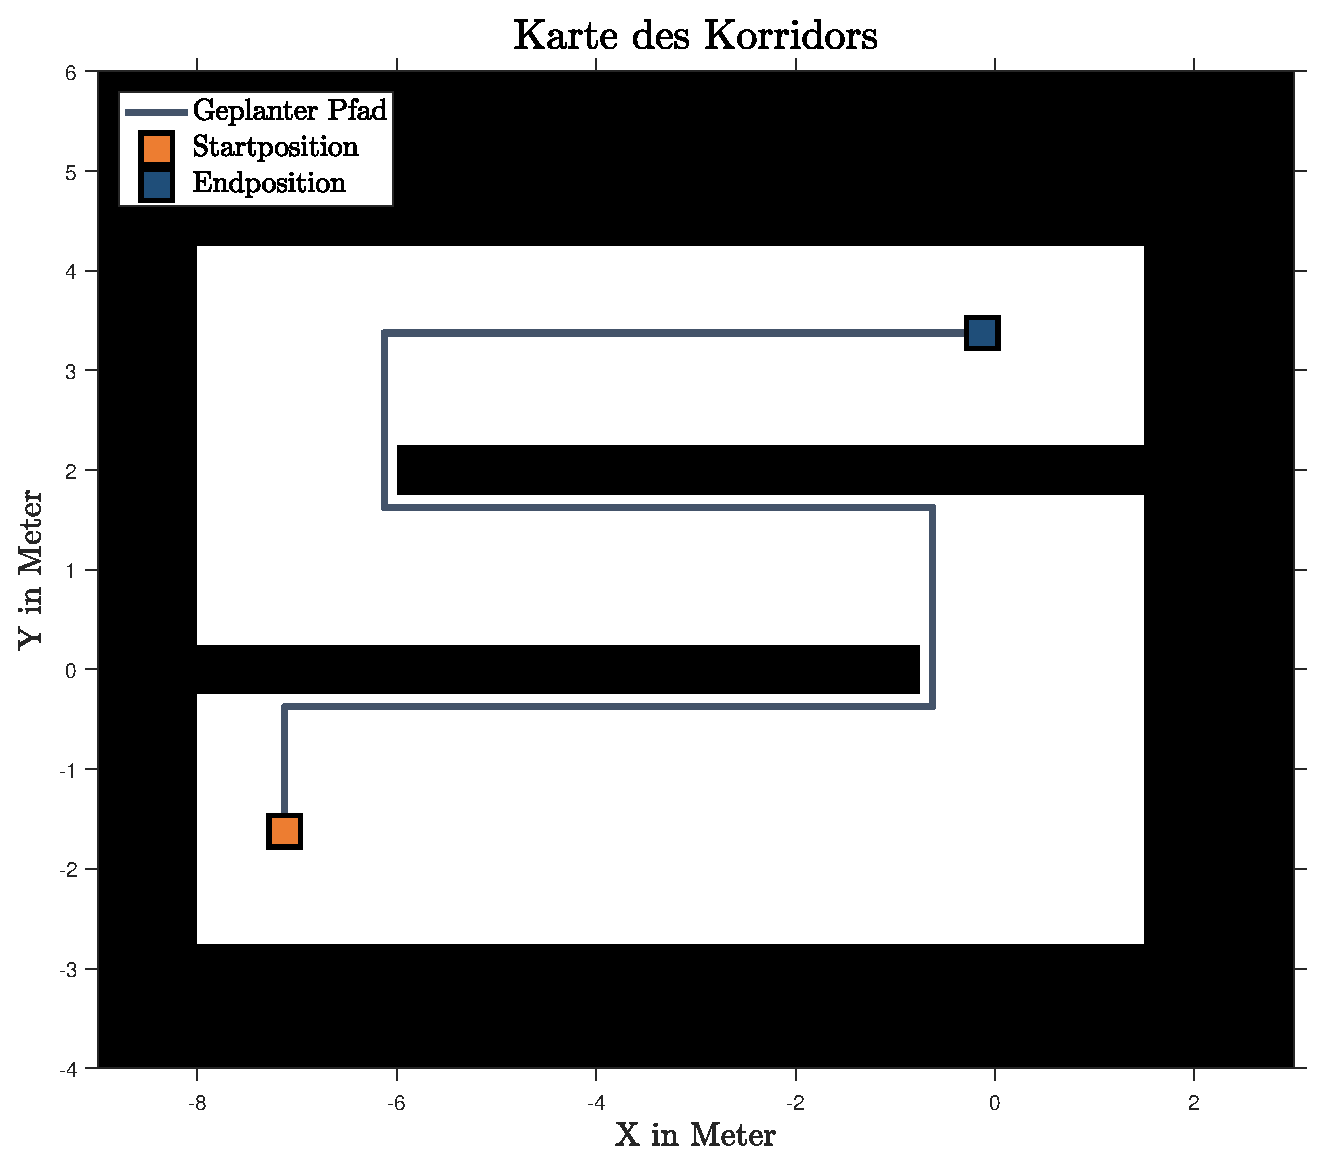
\includegraphics[width=0.7\linewidth]{img/KorridorBeispiel_img1.eps}
\caption{Ergebnis der Breitensuche}
\end{figure}


\section{Forward-Search: Tiefensuche}\pdfcomment{Seitenumbruch?}
Die komplementäre Suchstrategie wird als Depth-First-Search bezeichnet, bei der zuerst die Tiefe des Suchbaums erforscht wird, bevor parallele Zweige überprüft werden. Die Umsetzung der Depth-First-Search erfolgt indem die Datenstruktur Q als LIFO-Speicher implementiert wird. Dadurch kann im Vergleich zu der Breadth-First-Search die Suchzeit unter Umständen drastisch reduziert werden, allerdings resultieren für gewöhnlich längere Pfade. Wenn die Anzahl der Iterationsschritte oder die Menge der zulässigen Zustände begrenzt sind, wird auch die Depth-First-Search zu einem systematischen Suchansatz. Das heißt der Algorithmus stößt garantiert auf ein Ergebnis, falls ein solches existiert. Durch das LIFO-Prinzip der Datenstruktur wird das Ergebnis der zuletzt ausgeführten Aktion unmittelbar weiterverfolgt. \pdfcomment{Wiederholung dadurch}Dadurch bekommt die Reihenfolge, in der die möglichen Aktionen $\mVec{u}$ appliziert werden, eine zentrale Bedeutung, \pdfcomment{Formulierung}da dadurch die Suchrichtung vorgegeben wird. Die folgenden Abbildungen zeigen die Auswirkungen einer veränderten Aktionsreihenfolge anhand des Korridorbeispiels.

\begin{figure}[ht!]
\centering
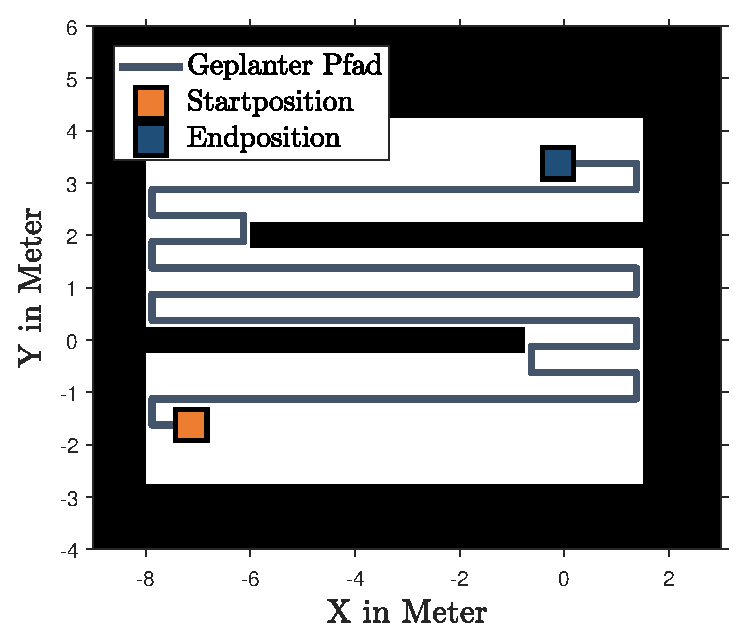
\includegraphics[width=0.45\linewidth]{img/KorridorBeispiel_img2.eps}
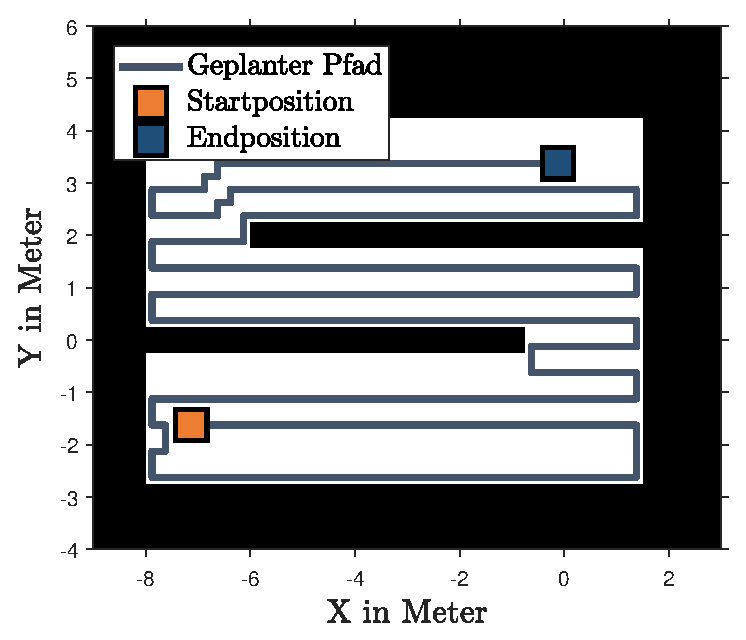
\includegraphics[width=0.45\linewidth]{img/KorridorBeispiel_img3.eps}

\vspace*{0.5cm}

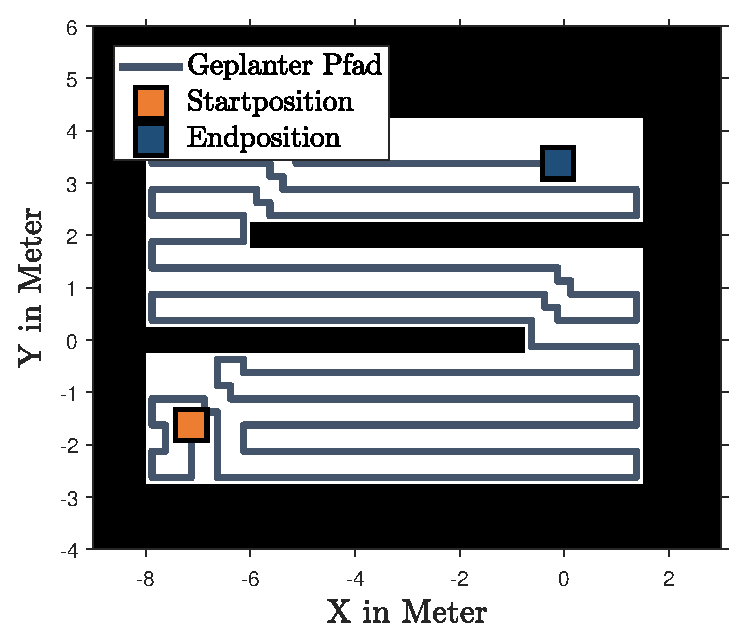
\includegraphics[width=0.45\linewidth]{img/KorridorBeispiel_img4.eps}
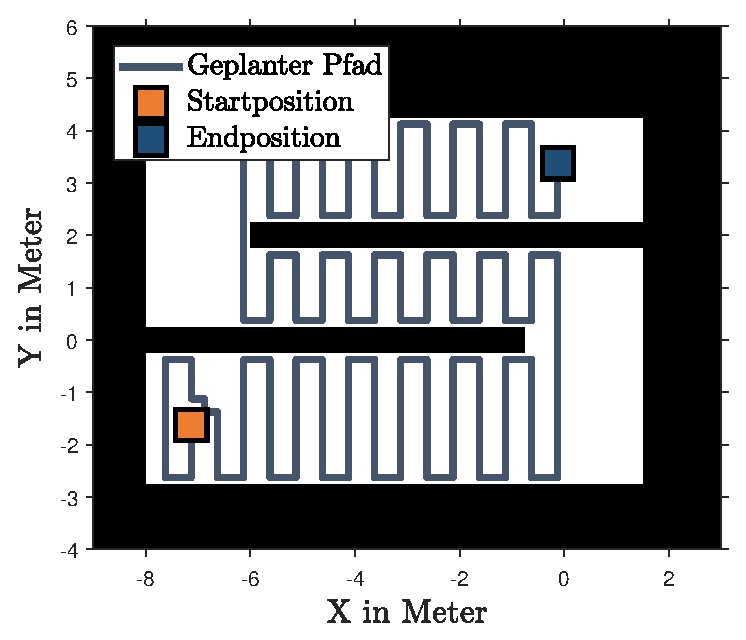
\includegraphics[width=0.45\linewidth]{img/KorridorBeispiel_img5.eps}
\caption{Ergebnisse der Tiefensuche bei unterschiedlichen Reihenfolge der Aktionen}
\end{figure}

Prinzipiell kann die Suche - unabhängig von der gewählten Strategie - auch von der Zielposition ausgehend beginnen. In diesem Fall wird von einer so genannten Backwards-Search gesprochen. Werden Forward- und Backward-Search simultan verfolgt, resultiert die so genannten Bidirectional-Search. Diese Adaptionen können unter Umständen verkürzte Suchzeiten liefern, werden an dieser Stelle aber nicht weiterverfolgt, da dieser Aspekt bei dem hiesigen Anwendungsfall nicht zum Tragen kommt.

\section{Optimale Suche und Planung}\pdfcomment{Idiotenapostroph und so}
In den bisherigen Suchalgorithmen bestand die Aufgabe lediglich darin,\pdfcomment{Alternativen für bestand darin} eine Pfad zwischen Ausgangs- und Zielposition zu finden. Dies hatte unter anderem zur Folge, dass starke Unterschiede zwischen den Lösungen der verschiedenen Ansätze resultierten. Besonders bei der Depth-First-Search kamen zum Teil äußerst umständliche Pfade zu Stande. Aus diesem Grund soll im nächsten Schritt eine Bewertung der Lösungsmöglichkeiten eingeführt werden, die genutzt wird, um einen optimalen Pfad im Sinne dieses Gütekriteriums zu ermitteln. Bei der globalen Pfadplanung sollen prinzipiell zwei Aspekte beachtet werden: Einerseits soll der resultierende Pfad möglichst kurz sein, andererseits soll ein gewisser Abstand zu belegten Zellen der Karte gehalten werden bzw. die belegten Zellen sollen von dem Pfad nicht durchkreuzt werden. Um diese Vorgaben in einem Gütekriterium auszudrücken, wird die Karte in eine sogenannte Kostenkarte transformiert. Diese ordnet jeder Zelle einen Aufwand zu, wodurch es möglich wird verschiedenen Pfade zu bewerten und miteinander zu vergleichen. Die Kosten eines Pfades ergeben sich aus der Summe der enthaltenen Zellen. Ein Beispiel für eine mögliche Bewertung der Zellen ordnet jeder freien Zelle den Aufwand $1$ und jeder belegten Zelle den Wert $\infty$ zu. Durch letzteren wird sichergestellt, dass belegte Zellen vermieden werden. Die Gewichtung von freien Zellen führt dazu, dass kürzere Pfade mit geringeren Kosten verbunden sind. Eine Möglichkeit, um einen im Kontext der Kostenkarte optimalen Pfad zu berechnen, stellt Dijkstra's Algorithmus dar. Dieser gleicht im Grundprinzip den bisher betrachteten Vorgehensweise, mit dem Unterschied, dass die Datenstruktur $Q$ so sortiert wird, dass das Element mit den aktuell geringstem Kostenaufwand am Anfang der Liste steht. Zusätzlich muss in dem Fall, dass ein Zustand geprüft wird, der bereits besucht worden ist, verglichen werden, welcher der beiden Pfade den geringeren Aufwand benötigt.

\begin{lstlisting}[mathescape=true, caption={Dijkstra's Algorithmus in Pseudocode}]
Q.Insert($\mVec{x}\idx{0}$) and mark $\mVec{x}\idx{0}$ as visited
while Q not empty do
	$\mVec{x}\idx{n}$ = Q.GetFirst()
	if $\mVec{x}\idx{n} = \mVec{x}\idx{G}$
		return SUCCESS
	forall $\mVec{u}  \in U$
		if $\mVec{x}\idx{n+1}$ not visited
			Mark $\mVec{x}\idx{n+1}$ as visited
			Q.Insert($\mVec{x}\idx{n+1}$)
		else
			resolve duplicate
return FAILURE
\end{lstlisting}
Die folgende Abbildung zeigt die Ergebnisse der Suche bei dem bekannten Anwendungsbeispiel.
\begin{figure}[ht!]
\centering
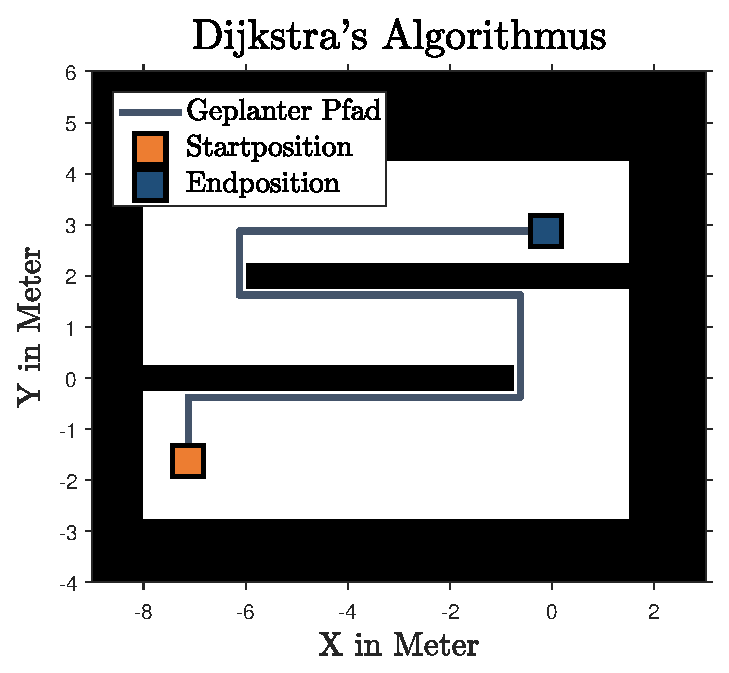
\includegraphics[width=0.5\linewidth]{img/KorridorBeispiel_img6.eps}
\caption{Ergebnis mit Dijkstra's Algorithmus}
\end{figure}

\subsection{A*}
Indem bei Dijakstra's Algorithmus die Liste $Q$ nach aufsteigenden Kosten sortiert wird, kann gesichert werden, dass die Suche zu einem optimalen Ergebnis führt. Allerdings bringt dieses Vorgehen einen zum Teil unnötigen Suchaufwand mit sich, was recht leicht illustriert werden kann: Um möglichst kurze Pfade zu erhalten, wurde jeder weitere Schritt mit einem fixen Aufwand bewertet. Dies hat zur Folge, dass die kürzesten Pläne an den Anfang der Liste rücken, inklusive der Pfade, die entweder zu kurz sind, um das Ziel überhaupt erreichen zu können, \pdfcomment{Formulierung}als auch solche die sich in eine falsche Richtung bewegen. Insofern erzwingt die sortierte Datenstruktur eine Breitensuche, da kurze Pfade fälschlicherweise - zumindest teilweise fälschlicherweise - mit weniger Aufwand verbunden sind.

Ein Ansatz, um dieser Problematik vorzubeugen, stellt der $A*$ Algorithmus dar, der nach dem identischen Grundprinzip wie Dijakstra's Algorithmus arbeitet. Lediglich das Gewichtungskonzept der Pläne unterscheiden die beiden Vorgehensweisen. Für jede Position $\mVec{x}\idx{n}$ existiert ein optimaler Pfad, welcher $\mVec{x}\idx{n}$ mit der Zielposition $\mVec{x}\idx{G}$ verbindet. Die Kosten des optimalen Pfades werden von der Funktion $G^*(\mVec{x}\idx{n})$ beschrieben\pdfcomment{Der Satz ist bisschen fehl am Platz}. Die Idee des $A*$ Algorithmus besteht darin, neben den Kosten des Pfades von $\mVec{x}\idx{0}$ zu $\mVec{x}\idx{n}$ auch die verbleibenden Kosten nach $\mVec{x}\idx{G}$ zu beachten. Dadurch werden kürzere Pfade nicht mehr aus Prinzip bevorzugt, sondern lediglich dann, wen ihre erwarteten Kosten bis zum Ziel ebenfalls gering sind. Da die optimalen Kosten $G^*(\mVec{x}\idx{n})$ nicht bekannt sind müssen sie approximiert werden, wofür eine heuristische Schätzung $G(\mVec{x}\idx{n})$ eingeführt wird. An die Heuristik ist die Beindung geknöpft, dass die geschätzten Kosten $G(\mVec{x}\idx{n})$ stets kleiner oder gleich der optimalen Kosten $G^*(\mVec{x}\idx{n})$ sind:
\begin{equation}
G(\mVec{x}\idx{n}) \leq G^*(\mVec{x}\idx{n}) \hspace{2.5cm} \forall \mVec{x}\idx{n} \in X\,.
\end{equation}
Als Beispiel wird wieder die Navigation durch den Korridor betrachtet. Hier wurde jede Verrückung mit dem Aufwand $1$ gewichtet, woraus folgt, dass die Kosten zwischen $\mVec{x}\idx{n}$ und $\mVec{x}\idx{G}$ mindestens gleich der absoluten Differenzen zwischen den X- und Y-Koordinaten der beiden Positionen sein muss. Im Falle, dass ein Hindernis den direkten Weg zwischen $\mVec{x}\idx{n}$ und $\mVec{x}\idx{G}$ versperrt nehmen die optimalen Kosten $G^*(\mVec{x}\idx{n})$ weiter zu, weshalb
\begin{equation}
G(\mVec{x}\idx{n}) = \vert x\idx{n} - x\idx{G}\vert + \vert y\idx{n} - y\idx{G}\vert \leq G^*(\mVec{x}\idx{n}) \hspace{2cm} \forall \mVec{x}\idx{n} \in X
\end{equation}
stets gilt. Somit stellt $G(\mVec{x}\idx{n})$ eine legitime Approximation der optimalen Kosten $G^*(\mVec{x}\idx{G})$ dar. Wird diese Forderung an die Kostenschätzung eingehalten, kann bewiesen werden, dass der $A*$ Algorithmus stets eine optimale Lösungs findet, insofern diese existiert \cite[S. 32]{PlanAlgo}\cite{SecRef1,SecRef2}. Bei der - recht konservativen - Schätzung $G(\mVec{x}\idx{n})=0$ geht das $A*$ Verfahren in Dijkstra's Algorithmus über.
\begin{figure}[ht!]
\centering
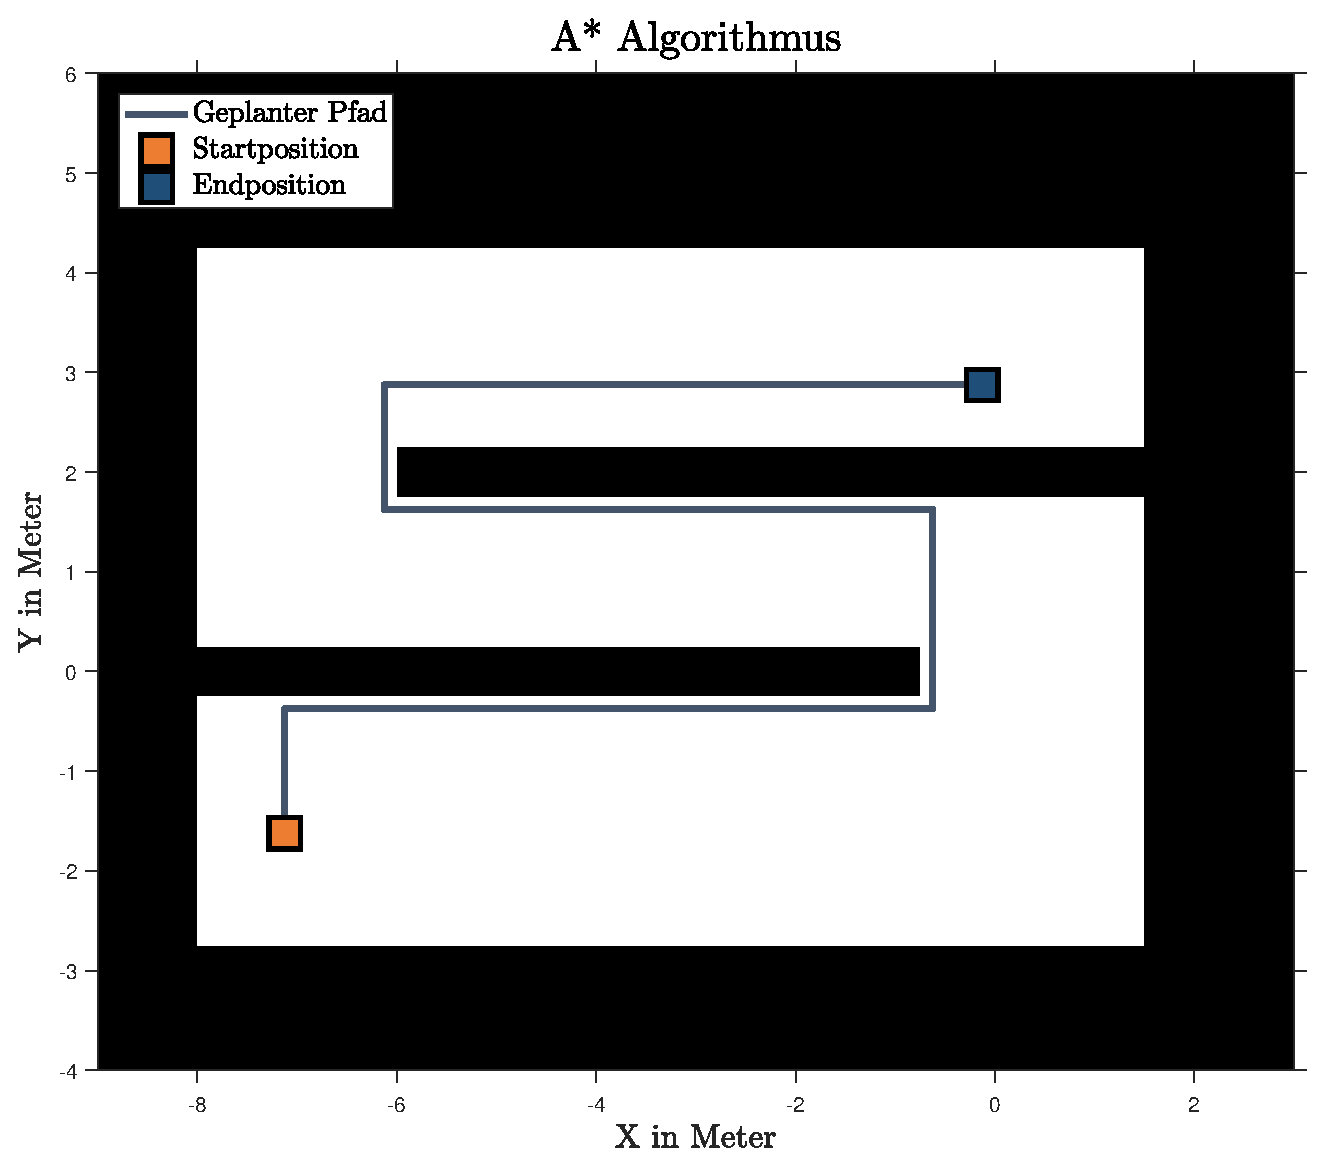
\includegraphics[width=0.5\linewidth]{img/KorridorBeispiel_img7.eps}
\caption{Ergebnis mit dem A* Algorithmus}
\end{figure}

\chapter{Stochastische Modelle in der Robotik}
Wie alle Probleme der Robotik, kann auch die autonome Navigation im entferntesten Sinne als Interaktion eines Roboters mit seiner Umwelt aufgefasst werden. Anhand von gesammelten Informationen muss das System eine Entscheidung über seine zukünftigen Aktionen treffen, wobei ein entferntes Ziel ohne ungewollte Kollisionen angesteuert werden soll. Für diese Aufgaben spielen drei Größen eine fundamentale Rolle. Zunächst muss die Position des Roboters beachtet werden, welche in dem Positionsvektor $\mVec{x}(t) \equiv \mVec{x}_t$ erfasst wird. Mithilfe von Sensoren sammelt der Roboter Informationen über seine Umgebung, die in dem Messvektor $\mVec{z}_t$ zusammengefasst werden. Anhand der Mess- und Positionsvektoren wird über die nächste Aktion des Roboters entschieden, die in dem Steuervektor $\mVec{u}_t$ ausgedrückt wird. Die exakte Form der Positions-, Mess- und Steuervektoren hängt von dem gegebenen Anwendungsfall und gewählten Modellformen ab, die im Folgenden näher erläutert werden.

In anderen Fachgebieten, die sich mit der Planung von Steuersignalen bzw. -sequenzen beschäftigen - wie z.B. der Regelungstechnik -, haben sich modellbasierte Methoden bewährt. Zunächst wird auf Basis von physikalischen Gegebenheiten der Zusammenhang zwischen Steuer-, Zustands- und Messvektor hergeleitet, der anschließend genutzt wird, um eine Regelstrategie zu formulieren. Der resultierende Algorithmus berechnet die Stellgröße $\mVec{u}_t$, wofür die aktuellen Mess- und Zustandsvektoren herangezogen werden. Insofern liegt es nahe modellbasierte Ansätze auch bei Problemen der Robotik zu verfolgen. Allerdings kommt dort die ungemeine Komplexität der Problemstellung zu tragen, die sich recht leicht am Beispiel der Navigation illustrieren lässt: Als erstes muss ein Modell für den Einfluss des Stellvektors $\mVec{u}_t$ auf den Positionsvektor $\mVec{x}_t$ erstellt werden. Bei mobilen Roboterplattformen handelt es sich um mechanische Systeme mit mehreren Freiheitsgraden, womit die analytische Modellbildung zwar möglich, jedoch mit einem beachtlichen Aufwand verbunden ist. Spätestens bei der Modellierung der Sensoren werden die Grenzen des Möglichen erreicht: Soll beispielsweise die Position des Roboters mithilfe von Stereokameras erfasst werden kann praktisch kaum ein exaktes, deterministisches Modell für diesen Vorgang erfasst werden, da er von zu vielen unbekannten Einflussfaktoren betroffen ist. Zuletzt kann die Pfadplanung per Definition nicht anhand eines deterministischen Modell erfolgen, da der Roboter dynamischen Hindernissen ausweichen soll, deren Form und Bewegung in der Aufgabenstellung nicht näher spezifiziert werden.

Aus diesen Gründen haben sich in der Robotik stochastische Modellformen etabliert, wobei recht simple Ausgangsmodelle verwendet werden, die um Zufallsvariablen ergänzt werden, um die Ungenauigkeiten und Ungewissheiten des Modells zu repräsentieren. Das Ziel besteht nicht mehr darin, konkrete Aussagen über den Verlauf von Zustandsgrößen zu treffen, wie dies z.B. bei einer Zustandsraumdarstellung der Form
\begin{equation}
\mVec{x}(n+1) = \mat{{A}}\cdot \mVec{x}(n) + \mat{B}\cdot \mVec{\mathbf{u}}(n)
\end{equation}
erfolgt. Vielmehr soll mithilfe des Modells eine bedingte Wahrscheinlichkeit
\begin{equation}
\condP{\mVec{x}(n+1)}{\mVec{x}(n), \mVec{u}(n)}
\end{equation}
berechnet werden. Im Anschluss können die Methoden der Wahrscheinlichkeitstheorie genutzt werden, um Filter- und Planungsalgorithmen zu entwerfen.\pdfcomment{Wiederholung der um.. Konstruktion} Um einen ersten Eindruck für diese Modellformen zu erhalten, werden im Anschluss rudimentäre Ansätze für ein Bewegungs- und Sensormodell vorgestellt.


\newpage
\section{Geschwindigkeitsbasiertes Bewegungsmodell } \footnote{Das Bewegungsmodell und dessen Herleitung stammen aus \cite[S. 121 ff]{ProbRob}} 
Als erstes Beispiel wird ein stochastisches Modell für die Roboterbewegung entworfen, wobei anhand des vergangenen Positionsvektor $\mVec{x}_{t-1}$ und des aktuellen Steuervektors $\mVec{u}_t$ die Wahrscheinlichkeitsverteilung des aktuellen Positionsvektors $\mVec{x}_t$
\begin{equation}
\condP{\mVec{x}_t}{\mVec{u}_t, \mVec{x}_{t-1}}
\end{equation}
bestimmt werden soll. In diesem Fall wird lediglich eine planare Bewegung betrachtet, das heißt der Roboter bewegt sich in der xy-Ebene. Der Positionsvektor setzt sich somit aus den drei Größen
\begin{equation}
\mVec{x} = \begin{pmatrix}
x \\ y \\ \theta
\end{pmatrix}
\end{equation}
zusammen, welche die x-/y-Position und Ausrichtung des Roboters wiedergeben. $\theta$ gibt dabei den Winkel zwischen der x-Koordinatenachse und der Blickrichtung des Roboters an.
Der Steuervektor $\mVec{u}$ gibt die aktuelle Translations- und Rotationsgeschwindigkeit
\begin{equation}
\mVec{u} = \begin{pmatrix}
v \\ \omega
\end{pmatrix}
\end{equation}
des Roboters an, wobei angenommen wird, dass die beiden Geschwindigkeiten zwischen zwei Abtastpunkten $t$ und $t+1$ konstant sind. $v$ beschreibt die Translationsgeschwindigkeit in Blickrichtung, während $\omega$ die Änderung des Blickwinkels $\theta$ wiedergibt.
Unter der Annahme dass die Geschwindigkeiten $\mVec{u}$ in dem Intervall $]t-1, t]$ zwischen zwei Abtastpunkten konstant bleibt, kann die Bewegung als Rotation um einen konstanten Momentanpol $\mVec{c} = \begin{pmatrix} x_c & y_c \end{pmatrix}^T$ betrachtet werden.
\begin{figure}[!ht]
\centering
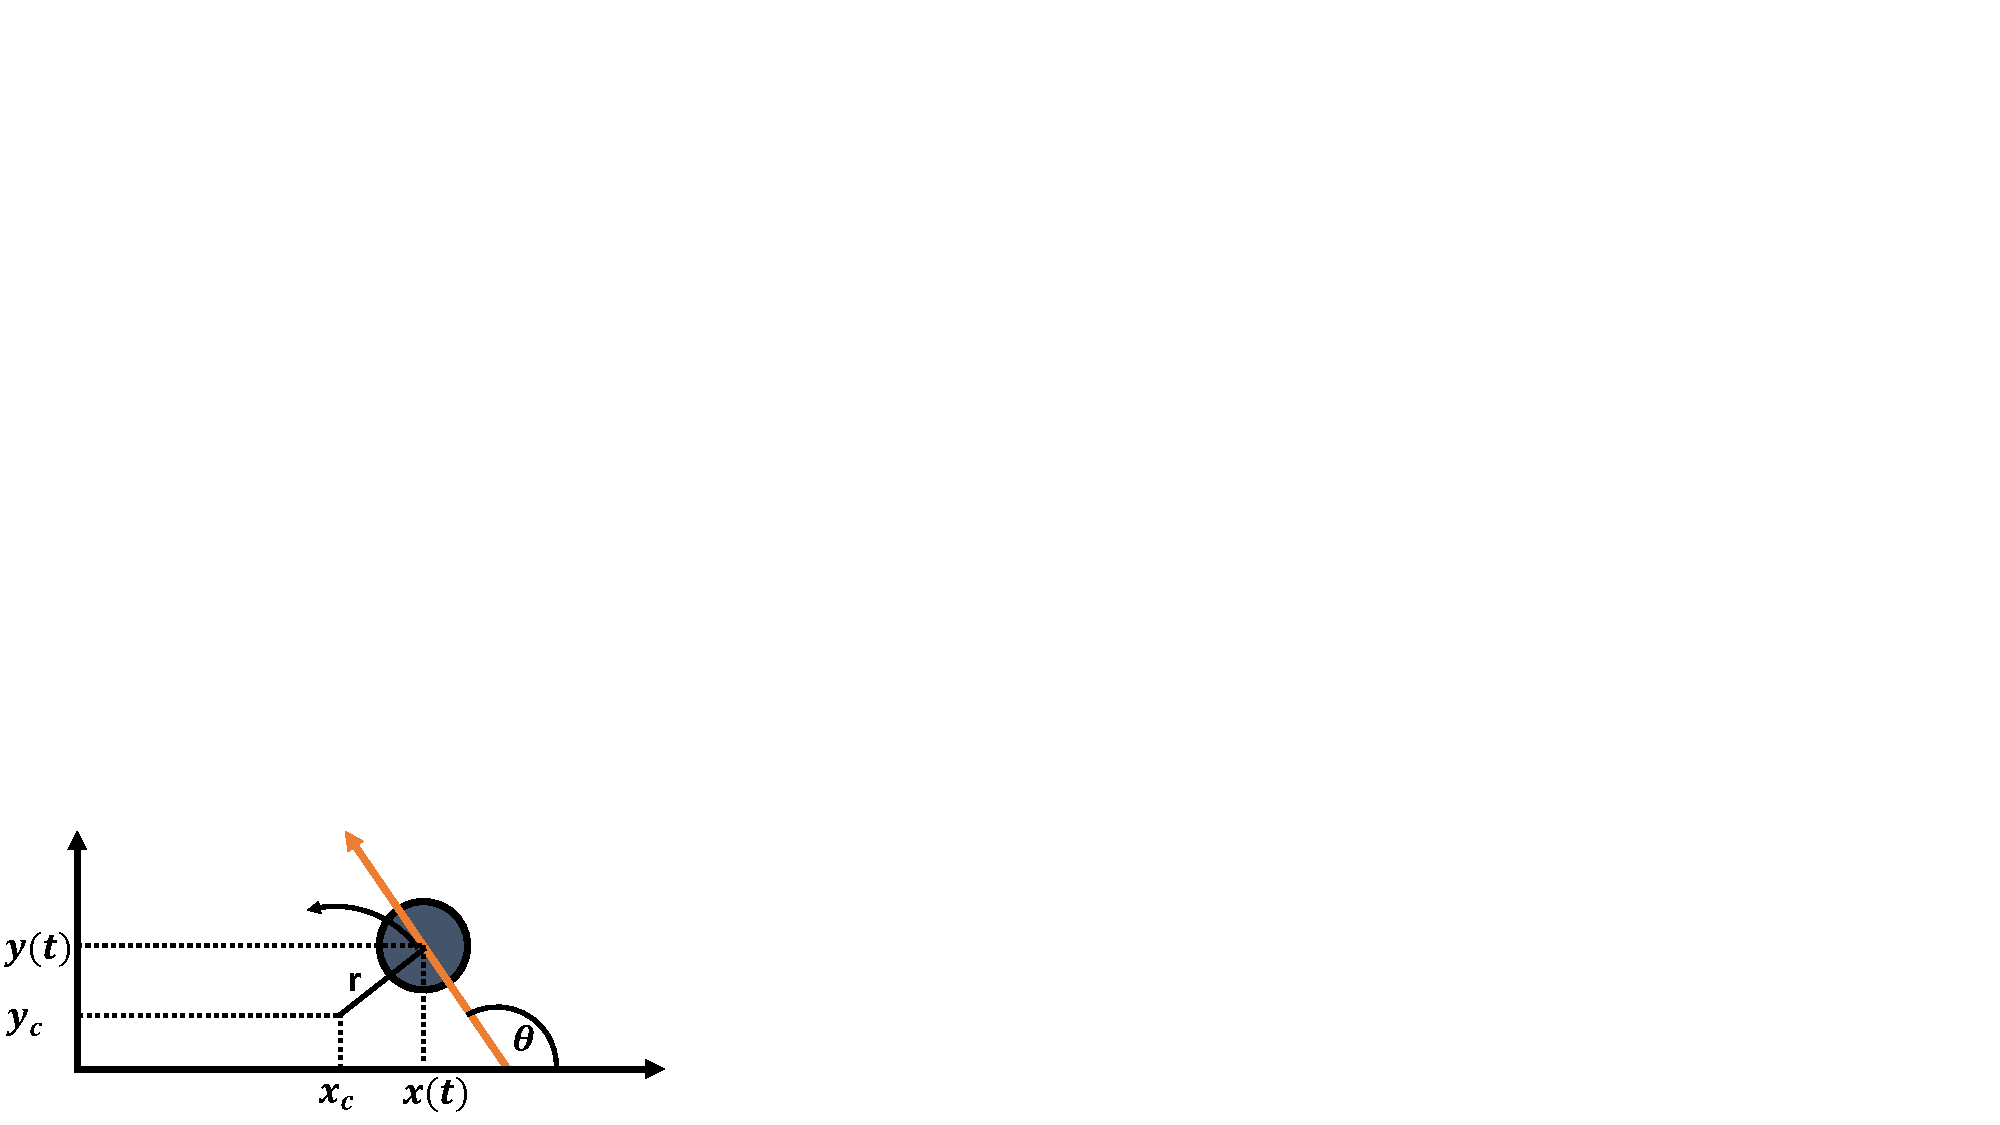
\includegraphics[width=0.6\linewidth, trim={0cm 0cm 24cm 14cm}, clip]{img/Bild_Kinematik_1}
\caption{Darstellung des Momentanpols am Zeitpunkt $t$ \cite[S. 126]{ProbRob}}
\end{figure}

Für den Radius gilt
\begin{equation}
r = \left\vert \frac{v}{\omega}\right\vert\,,
\end{equation}
wobei zu beachten ist, dass der Radius für eine Winkelgeschwindigkeit $\omega=0$ gegen unendlich konvergiert, was wiederum einer reinen Translation entspricht. Aus dem Positionsvektors des Roboters $\mVec{x}_t$ an dem Zeitpunkt $t$ kann der Momentanpol für die folgende Abtastperiode berechnet werden:
\begin{equation}
\label{eq_kinematic_1}
\begin{pmatrix}
x_c \\ y_c
\end{pmatrix} = \begin{pmatrix}
x(t) - \frac{v}{\omega}\cdot \mySin{\theta} \\ y(t) + \frac{v}{\omega}\cdot \myCos{\theta}
\end{pmatrix} \hspace{15pt}\leftrightarrow\hspace{15pt} 
\begin{pmatrix}
x(t) \\ y(t)
\end{pmatrix} = \begin{pmatrix}
x_c + \frac{v}{w}\cdot \mySin{\theta} \\ y_c - \frac{v}{w}\cdot \myCos{\theta}
\end{pmatrix}\,.
\end{equation}
Im nächsten Schritt wird die Bewegung über eine Abtastperiode $\Delta t$ betrachtet, wodurch der Roboter um die Winkeldifferenz $\Delta t\cdot \omega$ auf dem Kreisbogen wandert. Nach \ref{eq_kinematic_1} folgt für den Positionsvektor am Zeitpunkt $t+\Delta t$
\begin{equation}
\label{eq_kinematic_2}
\begin{split}
\begin{pmatrix}
x(t+\Delta t) \\ y(t+\Delta t) \\ \theta(t+\Delta t
\end{pmatrix} &= \begin{pmatrix}
x_c + \frac{v}{w}\cdot \mySin{\theta(t)+\omega\cdot \Delta t} \\ y_c - \frac{v}{w}\cdot \myCos{\theta(t)+\omega \cdot \Delta t} \\ \theta(t) + \omega\cdot \Delta t
\end{pmatrix}\\
& = \begin{pmatrix}
x(t) \\ y(t) \\ \theta(t)
\end{pmatrix} + \begin{pmatrix}
-\frac{v}{\omega}\cdot\mySin{\theta(t)} + \frac{v}{\omega}\cdot \mySin{\theta(t)+\omega \cdot \Delta t} \\
\frac{v}{\omega}\cdot \myCos{\theta(t)} - \frac{v}{w}\cdot \myCos{\theta(t)+\omega \cdot \Delta t}\\
\omega\cdot \Delta t
\end{pmatrix}\,.
\end{split}
\end{equation}
Bisher wurden lediglich deterministische Bewegungen betrachtet. Um nun mögliche Fehler des Steuervektors $\mVec{u}$ zu beachten, werden die störbehafteten Geschwindigkeiten
\begin{equation}
\mVec{u} = \begin{pmatrix}
\hat{v} \\ \hat{\omega}
\end{pmatrix} = \begin{pmatrix}
v + v\idx{err} \\ \omega + \omega\idx{err}
\end{pmatrix}
\end{equation}
eingeführt. Die Zufallsvariablen $v\idx{err}$ und $\omega\idx{err}$ dienen der Fehlermodellierung und ihre Wahrscheinlichkeitsverteilungen $\varepsilon_v$ und $\varepsilon_\omega$ werden dem Anwendungsfall nach angepasst. Einsetzen des stochastischen Steuervektors $\mVec{u}$ liefert
\begin{equation}
\begin{pmatrix}
x(t+\Delta t) \\ y(t+\Delta t) \\ \theta(t+\Delta t
\end{pmatrix} 
=
\begin{pmatrix}
x(t) \\ y(t) \\ \theta(t)
\end{pmatrix} + \begin{pmatrix}
-\frac{\hat{v}}{\hat{\omega}}\cdot\mySin{\theta(t)} + \frac{\hat{v}}{\hat{\omega}}\cdot \mySin{\theta(t)+\hat{\omega} \cdot \Delta t} \\
\frac{\hat{v}}{\hat{\omega}}\cdot \myCos{\theta(t)} - \frac{\hat{v}}{w}\cdot \myCos{\theta(t)+\hat{\omega} \cdot \Delta t}\\
\hat{\omega}\cdot \Delta t
\end{pmatrix}\,.
\end{equation}
In diesem Modell wurden lediglich zwei Zufallsvariablen eingeführt, um die Störung von drei Positionsvariablen zu modellieren. Aus diesem Grund entsteht eine ungewollte stochastische Abhängigkeit zwischen den Elementen des Positionsvektors $\mVec{x}(t+\Delta t)$. Dieses Problem wird behoben, indem eine dritte Zufallsvariable
\begin{equation}
\gamma\idx{err} \equiv \hat{\gamma}
\end{equation}
eingeführt wird, die zu einer zusätzlichen Störung der Orientierung $\theta(t+\Delta t)$ in Form von
\begin{equation}
\label{eq_kinematic_3}
\begin{pmatrix}
x(t+\Delta t) \\ y(t+\Delta t) \\ \theta(t+\Delta t
\end{pmatrix} 
=
\begin{pmatrix}
x(t) \\ y(t) \\ \theta(t)
\end{pmatrix} + \begin{pmatrix}
-\frac{\hat{v}}{\hat{\omega}}\cdot\mySin{\theta(t)} + \frac{\hat{v}}{\hat{\omega}}\cdot \mySin{\theta(t)+\hat{\omega} \cdot \Delta t} \\
\frac{\hat{v}}{\hat{\omega}}\cdot \myCos{\theta(t)} - \frac{\hat{v}}{w}\cdot \myCos{\theta(t)+\hat{\omega} \cdot \Delta t}\\
\hat{\omega}\cdot \Delta t + \hat{\gamma}\cdot \Delta t
\end{pmatrix}
\end{equation}
führt. Die Aufgabe besteht jetzt darin, ein Bewegungsmodell in Form der bedingten Wahrscheinlichkeit
\begin{equation}
\condP{\mVec{x}_t]}{\mVec{u}_t, \mVec{x}_{t-1}}
\end{equation}
zu formulieren. Das heißt es soll eine Funktion aufgestellt werden, die berechnet wie wahrscheinlich der Zustand $\mVec{x}_t$ auf den Zustand $\mVec{x}_{t-1}$ und die Aktion $\mVec{u}_t$ folgt. Dafür wird nach Gleichung (\ref{eq_kinematic_3}) die Werte der stochastisch unabhängigen Zufallsvariablen $v\idx{err}$, $\omega\idx{err}$ und $\gamma\idx{err}$ berechnet. Die gesuchte Wahrscheinlichkeit ergibt sich dann aus deren gemeinsamer Verteilung
\begin{equation}
p(\mVec{x}_t, \mVec{u}_t, \mVec{x}_{t-1}) = \condP{\mVec{x}_t}{\mVec{u}_t, \mVec{x}_{t-1}} = \varepsilon_v(v\idx{err})\cdot \varepsilon_\omega(\omega\idx{err})\cdot \varepsilon_\gamma(\gamma\idx{err})\,.
\end{equation}
Da die direkte Umformung von Gleichung (\ref{eq_kinematic_1}) zur expliziten Darstellung der gesuchten Fehlergrößen zu einem unhandlichen Ergebnis führt, wird eine indirekte Berechnung über den Momentanpol gewählt. Im ersten Schritt werden die Koordinaten des Momentanpols $\mVec{c}$ berechnet, wofür sich nach \cite[S. 130]{ProbRob} \footnote{Schreibweise für $\mVec{x}_t = \begin{pmatrix}
x & y &\theta
\end{pmatrix}^T$, $\mVec{x}_{t+\Delta t} = \begin{pmatrix}
\tilde{x} & \tilde{y} &\tilde{\theta}
\end{pmatrix}^T$}
\begin{equation}
\begin{pmatrix}
x_c \\ y_c
\end{pmatrix} = \begin{pmatrix}
\frac{x+\tilde{x}}{2} + \mu (y-\tilde{y})\\ \frac{y+\tilde{y}}{2}+\mu(\tilde{x}-x)
\end{pmatrix} \hspace{1.5cm}
\mu = \frac{1}{2}\frac{(x-\tilde{x})\myCos{\theta} + (y-\tilde{y})\mySin{\theta}}{(y-\tilde{y})\myCos{\theta}-(x-\tilde{x})\mySin{\theta}}
\end{equation}
ergibt. Woraus sich sowohl der Rotationsradius
\begin{equation}
r\idx{c} = \sqrt{(x-x_c)^2+(y-y_c)^2}
\end{equation}
als auch der auf der Kreisbahn zurückgelegte Winkel 
\begin{equation}
\Delta \theta = \myAtan{\frac{\tilde{y}-y_c}{\tilde{x}-x_c}}-\myAtan{\frac{y-y_c}{x-x_c}}
\end{equation}
berechnen lassen. Mithilfe der der Winkeldifferenz lässt sich wiederum auf die zurückgelegte Strecke
\begin{equation}
\Delta s = r\idx{c}\cdot \Delta \theta
\end{equation}
schließend, welche zusammen auf den gestörten Stellvektor
\begin{equation}
\mVec{\hat{u}} = \begin{pmatrix}
\hat{v}\\ \hat{\omega}
\end{pmatrix} = \frac{1}{\Delta t}\cdot \begin{pmatrix}
\Delta s\\ \Delta \theta
\end{pmatrix}
\end{equation}
führen. Zuletzt fehlt der Orientierungsfehler $\hat{\gamma}$, der sich mithilfe von Gleichung (\ref{eq_kinematic_3}) erschließen lässt.
\begin{equation}
\tilde{\theta}-\theta = \hat{\omega}\cdot \Delta t + \hat{\gamma}\cdot \Delta t
\Leftrightarrow
\hat{\gamma} = \frac{\tilde{\theta}-\theta}{\Delta t} - \hat{\omega}\,.
\end{equation}

\newpage
\section{Messmodell}
Als weiteres Beispiel wird ein stochastisches Messmodell vorgestellt, das später bei der Lokalisierung wiederverwendet wird. Das Ziel des Messmodells ist es den Zusammenhang zwischen einem Zustandsvektor $\mVec{x}\idx{t}$ und einem Messvektor $\mVec{z}\idx{t}$ in Form der bedingten Wahrscheinlichkeit
\begin{equation}
\condP{\mVec{z}\idx{t}}{\mVec{x}\idx{t}}
\end{equation}
herzustellen. Die Verteilung sagt aus, mit welcher Wahrscheinlichkeit ein Messvektor $\mVec{z}\idx{t}$ von einer vorgegebenen Position $\mVec{x}\idx{t}$ aus erzielt wird. Das Messmodell dient als Paradebeispiel dafür, wie heuristische Argumente in stochastische Modelle einfließen können. Unabhängig von dem exakten Sensor wird angenommen, dass es sich um ein auf Messstrahlen basiertes Messprinzip handelt. Das heißt der Messvektor $\mVec{z}\idx{t}$ setzt sich aus mehreren Messwerten $z^k\idx{t}$ zusammen, die jeweils die auf einem Strahl gemessene Distanz wiedergeben. 

Als erste Störgröße wird ein gewöhnliches Messrauschen eingeführt, das als normal verteilt angenommen wird. Der Mittelwert der Verteilung sie die tatsächliche Distanz auf dem Messstrahl, die mit $z^{k*}\idx{t}$ denotiert wird. Als zweiter Parameter muss die Varianz $\sigma\idx{hit}$ festgelegt werden, die angibt wie stark der Messwert von dem Rauschen beeinflusst wird. Somit ergibt sich als Modell für das Sensorrauschen
\begin{equation}
p\idx{hit}\left( z^{k}\idx{t} \mCond \mVec{x}\idx{t} \right) = \left\{ \begin{array}{cl}
\eta \cdot \mathcal{N}(z^k\idx{t}, z^{k*}\idx{t}, \sigma^2\idx{hit}) & \hspace{5mm}\forall z^k\idx{t} \in \left[0, z\idx{max}\right] \\
0 & \hspace{5mm} \forall z^k\idx{t} \notin \left[0, z\idx{max}\right]
\end{array}\right. \,.
\end{equation}
Die Messwerte werden außerdem von unerwarteten Objekten beeinflusst. Angenommen es liegt eine Karte der Umgebung vor und es bewegt sich ein Mensch innerhalb des Raumes. Wenn der Mensch nun die Messstrahlen unterbricht tritt ein geringerer Messwert als anhand der Karte erwartet ein. Im Allgemeinen gilt, dass im Falle von Störungen durch unerwartete Objekte die Messwerte lediglich kleiner, aber niemals größer werden. Des Weiteren nimmt die Wahrscheinlichkeit, dass ein Messwert von einem Objekt beeinflusst wird mit zunehmendem Messdistanz ab. Für das Modell wird eine exponentiell abfallende Verteilung
\begin{equation}
\renewcommand*{\arraystretch}{1.3}
p\idx{short}\left( z^k\idx{t} \mCond \mVec{x}\idx{t} \right) = \left\{ \begin{array}{cl}
\eta \cdot \lambda\idx{short}\cdot e^{-\lambda\idx{short}\cdot z^{k}\idx{t}} & \hspace{5mm} \forall z^{k}\idx{t} \in \left[0, z^{k*}\idx{t}\right] \\
0 & \hspace{5mm} \forall z^{k}\idx{t} \notin \left[0, z^{k*}\idx{t}\right]
\end{array}\right. 
\end{equation}
gewählt, wobei $\lambda\idx{short}$ als wählbarer Parameter die Häufigkeit der Störungen widerspiegelt.

Als dritte Ursache für Messfehler wird das sporadische Versagen des Sensors herangezogen. Derartige Phänomene können bei Laserscannern auftreten, wenn beispielsweise schwarze Oberflächen die Strahlen vollständig absorbieren. Ähnliche Probleme werden bei Sonarsensoren durch Interferenz oder schallabsorbierende Medien hervorgerufen. Unabhängig von dem Messprinzip des Sensors werden in all den beschriebenen Fällen - fälschlicherweise - maximale Distanzen gemessen, wodurch die Verteilung
\begin{equation}
p\idx{max}\left(z^k\idx{t} \mCond \mVec{x}\idx{t}\right) = \left\{ \begin{array}{cl}
1 & \hspace{5mm} \forall z = z\idx{max} \\
0 & \hspace{5mm} \forall z  \neq z\idx{max}
\end{array}\right.
\end{equation}
motiviert wird. {\color{red} Die Aussage von dieser Verteilung ist ein bisschen Banane, wenn wenn der Messwert den maximal Möglichen anzeigt, ist die dass 100 Prozent der Fall, ansonsten nicht? Oder ist es so zu verstehen, dass ein maximaler Messwert zu 100 Prozent den Fall von Messfehler bedeutet? Dann müsste ich die Interpretation der anderen Verteilungen nochmal überdenken}

Als letzter und absurdester Fall werden rein zufällig falsche Phänomene betrachtet. Als Argument dient die Beobachtung, dass es unerklärliche Messwerte gibt, die - zu Gunsten der Simplizität - durch eine Gleichverteilung der Form
\begin{equation}
\renewcommand*{\arraystretch}{1.3}
p\idx{rand}\left( z^k\idx{t} \mCond \mVec{x}\idx{t}\right) = \left\{ \begin{array}{cl}
\frac{1}{z\idx{max}} & \hspace{5mm} \forall z^k\idx{t} \in \left[0, z\idx{max}\right] 
\\
0 & \hspace{5mm} \forall z^k\idx{t} \notin \left[0, z\idx{max}\right]
\end{array} \right.
\end{equation}
repräsentiert werden. Es liegt schließlich nahe das komplexeste aller Probleme durch die simpelste aller Darstellung zu beschreiben. An diesem Beispiel wird deutlich, dass heuristische Einflüsse in stochastischen Modellen auch mit variierendem Elan verteidigt werden.

Die gesuchte Wahrscheinlichkeit $\condP{z^k\idx{t}}{\mVec{x}\idx{t}}$ wird aus Summe der vier Verteilung berechnet, wobei diese mit den Faktoren $z\idx{hit}$, $z\idx{short}$, $z\idx{max}$ und $z\idx{rand}$ gewichtet werden. Die Gewichtung erlauben es dem Anwender, die Heuristiken nach ihrer Glaubhaftigkeit zu bewerten.
\begin{equation}
\condP{z^k\idx{t}}{\mVec{x}\idx{t}} = \begin{bmatrix} z\idx{hit} & z\idx{short} & z\idx{max} z\idx{rand} \end{bmatrix} \cdot \begin{bmatrix}
p\idx{hit}\left( z^{k}\idx{t} \mCond \mVec{x}\idx{t} \right) \\
p\idx{short}\left( z^k\idx{t} \mCond \mVec{x}\idx{t} \right) \\
p\idx{max}\left(z^k\idx{t} \mCond \mVec{x}\idx{t}\right) \\
p\idx{rand}\left( z^k\idx{t} \mCond \mVec{x}\idx{t}\right)
\end{bmatrix}\,.
\end{equation}
\newpage
\section{Kontinuierliches Bayes Filter}
In der Robotik werden stochastische Filter genutzt, um anhand von gegebenen Information wie Mess- und Stellgrößen eine Schätzung über unbekannte Zustände des Systems zu treffen. Die Grundlage für derartige Methoden stellt das Bayes-Filter für kontinuierlich verteilte Zustände dar. Als Beispiel für die Herleitung und Illustration des Filters wird die Lokalisierungsaufgabe herangezogen, bei welcher die aktuelle Position $\mVec{x}\idx{t}$ des Roboters ermittelt werden soll. Die Schätzung stützt sich dabei auf die bisher gesammelten Messwerte $\mVec{z}\idx{1:t}$ und Stellgrößen $\mVec{u}\idx{1:t}$. Insofern kann die Lokalisierungsaufgabe als die Bestimmung der bedingten Wahrscheinlichkeit
\begin{equation}
\condP{\mVec{x}\idx{t}}{\mVec{z}\idx{1:t},\mVec{u}\idx{1:t}}
\end{equation}
reformuliert werden, die im Folgenden auch mittels der Definition
\begin{equation}
\bel{\mVec{x}\idx{t}} \equiv \condP{\mVec{x}\idx{t}}{\mVec{z}\idx{1:t},\mVec{u}\idx{1:t}}
\end{equation}
abgekürzt wird. Im Falle, dass der aktuelle Messwert $\mVec{z}\idx{t}$ bei der Verteilung nicht beachtet wird, gilt
\begin{equation}
\pbel{\mVec{x}\idx{t}} \equiv \condP{\mVec{x}\idx{t}}{\mVec{z}\idx{1:t-1},\mVec{u}\idx{1:t}}\,.
\end{equation}
Für die Bestimmung der Filtergleichungen wird auf Bayes Theorem zurückgegriffen:
\begin{equation}
\begin{split}
\bel{\mVec{x}\idx{t}} &= \condP{\mVec{x}\idx{t}}{\mVec{z}\idx{t},\mVec{z}\idx{1:t-1},\mVec{u}\idx{1:t}} = \frac{ \condP{\mVec{z}\idx{t}}{\mVec{x}\idx{t},\mVec{z}\idx{1:t-1},\mVec{u}\idx{1:t}}\cdot \condP{\mVec{x}\idx{t}}{\mVec{z}\idx{1:t-1},\mVec{u}\idx{1:t}}}{\condP{\mVec{z}\idx{t}}{\mVec{z}\idx{1:t-1}, \mVec{u}\idx{1:t}}}
\\
&= \mu \cdot \condP{\mVec{z}\idx{t}}{\mVec{x}\idx{t},\mVec{z}\idx{1:t-1},\mVec{u}\idx{1:t}}\cdot \condP{\mVec{x}\idx{t}}{\mVec{z}\idx{1:t-1},\mVec{u}\idx{1:t}}\,.
\end{split}
\end{equation}
Der Einfluss der bedingte Wahrscheinlichkeit $\condP{\mVec{z}\idx{t}}{\mVec{z}\idx{1:t-1}, \mVec{u}\idx{1:t}}$ wird dabei durch den Faktor $\mu$ ersetzt, der für die Normalisierung reserviert wird, um sicherzustellen, dass es sich bei $\pbel{\mVec{x}\idx{t}}$ um eine legitime Wahrscheinlichkeitsverteilung handelt. Eine weitere Vereinfachung basiert auf der Annahme, dass $\mVec{x}\idx{t}$ einen so genannten vollständigen Zustand darstellt, das heißt $\mVec{x}\idx{t}$ beinhaltet bereits alle vergangen Information. Aus diesem Grund verändern zusätzliche Informationen aus vergangen Mess- und Stellgrößen eine mit $\mVec{x}\idx{t}$ bedingte Wahrscheinlichkeit nicht, woraus 
\begin{equation}
\condP{\mVec{z}\idx{t}}{\mVec{x}\idx{t},\mVec{z}\idx{1:t-1},\mVec{u}\idx{1:t}} = \condP{\mVec{z}\idx{t}}{\mVec{x}\idx{t}}
\end{equation}
resultiert. Wird dieses Ergebnis in die ursprüngliche Gleichung eingesetzt, ergibt sich
\begin{equation}
\label{eq_contbayes2}
\begin{split}
\bel{\mVec{x}\idx{t}} &= \mu \cdot \condP{\mVec{z}\idx{t}}{\mVec{x}\idx{t}}\cdot \condP{\mVec{x}\idx{t}}{\mVec{z}\idx{1:t-1},\mVec{u}\idx{1:t}} 
\\
&= \mu \cdot \condP{\mVec{z}\idx{t}}{\mVec{x}\idx{t}}\cdot \pbel{\mVec{x}\idx{t}}\,.
\end{split}
\end{equation}
Mithilfe von weiteren Annahmen kann auch die Wahrscheinlichkeit $\pbel{\mVec{x}\idx{t}}$ ermittelt werden, wofür diese zunächst erweitert wird.
\begin{equation}
\label{eq_pbel}
\begin{split}
\pbel{\mVec{x}\idx{t}} &= \condP{\mVec{x}\idx{t}}{\mVec{z}\idx{1:t},\mVec{u}\idx{1:t}}
\\
&= \int \condP{\mVec{x}\idx{t}}{\mVec{x}\idx{t-1},\mVec{z}\idx{1:t-1},\mVec{u}\idx{1:t}}\cdot \condP{\mVec{x}\idx{t-1}}{\mVec{z}\idx{1:t-1},\mVec{u}\idx{1:t}}d\mVec{x}\idx{t-1}\,.
\end{split}
\end{equation}
Falls $\mVec{x}\idx{t-1}$ ebenfalls ein vollständiger Zustand ist kann eine Vereinfachung der Form
\begin{equation}
\label{eq_sub1}
\condP{\mVec{x}\idx{t}}{\mVec{x}\idx{t-1},\mVec{z}\idx{1:t-1},\mVec{u}\idx{1:t}}=\condP{\mVec{x}\idx{t}}{\mVec{x}\idx{t-1},\mVec{u}\idx{t}}
\end{equation}
durchgeführt werden. Wenn zusätzlich angenommen werden kann, dass $\mVec{u}\idx{t}$ zufällig gewählt wird und somit kein Zusammenhang zwischen $\mVec{x}\idx{t-1}$ und $\mVec{u}\idx{t}$ besteht, folgt
\begin{equation}
\label{eq_sub2}
\condP{\mVec{x}\idx{t-1}}{\mVec{z}\idx{1:t-1},\mVec{u}\idx{1:t}} = \condP{\mVec{x}\idx{t-1}}{\mVec{z}\idx{1:t-1},\mVec{u}\idx{1:t-1}} = \bel{\mVec{x}\idx{t-1}}\,.
\end{equation}
Die Substitution der beiden Ergebnisse (\ref{eq_sub1}) und (\ref{eq_sub2}) in Gleichung (\ref{eq_pbel}) liefert
\begin{equation}
\label{eq_contbayes1}
\pbel{\mVec{x}\idx{t}} = \int \condP{\mVec{x}\idx{t}}{\mVec{x}\idx{t-1},\mVec{u}\idx{t}}\cdot \bel{\mVec{x}\idx{t-1}}d\mVec{x}\idx{t-1}
\end{equation}
und bildet zusammen mit Gleichung (\ref{eq_contbayes2}) die folgende Berechnungsvorschrift des Bayes-Filter.
\begin{lstlisting}[mathescape=true, caption={Bayes-Filter},captionpos=b]
Algorithm: BayesFilter($\bel{\mVec{x}\idx{t-1}},\mVec{u}\idx{t},\mVec{z}\idx{t}$):
	for all $\mVec{x}\idx{t}$ do:
		$\pbel{\mVec{x}\idx{t}} = \int \condP{\mVec{x}\idx{t}}{\mVec{x}\idx{t-1},\mVec{u}\idx{t}}\cdot \bel{\mVec{x}\idx{t-1}}d\mVec{x}\idx{t-1}$
		$\bel{\mVec{x}\idx{t}} = \mu \cdot \condP{\mVec{z}\idx{t}}{\mVec{x}\idx{t}}\cdot \pbel{\mVec{x}\idx{t}}$
	endfor
	return $\bel{\mVec{x}\idx{t}}$
\end{lstlisting}

\newpage
\subsection*{Applikation, Interpretation und kritische Anmerkungen}
Die bisherige Untersuchung hat sich auf die Herleitung der Berechnungsvorschrift und deren mathematischen Gültigkeit beschränkt, weshalb an dieser Stelle die Ergebnisse auf die konkrete Problemstellung der Lokalisierung übertragen werden. Dafür werden zunächst die Argumente des Algorithmus betrachtet: Bei den Vektoren $\mVec{u}\idx{t}$ und $\mVec{z}\idx{t}$ handelt es sich um die aktuellen Stell- und Messwerte. Der Erstgenannte enthält für gewöhnlich die aktuelle Geschwindigkeit des Roboters. In $\mVec{z}\idx{t}$ werden die aktuellen Sensorinformationen zusammengefasst, wobei es sich in diesem Fall um Distanzmessungen handelt, die mit einem Laserscanner gewonnen wurden. Das dritte Argument enthält die Wahrscheinlichkeit $\bel{\mVec{x}\idx{t-1}}$ am vorherigen Abtastzeitpunkt, die für den Fall $\mVec{x}\idx{0}$ initialisiert werden muss. Bei der Wahl der Startverteilung wird auf a priori Kenntnisse und Heuristiken zurückgegriffen. Beispielsweise kann der Anwender anhand einer Karte Positionen, die von einem Hindernis belegt sind, vorab ausschließen. Liegen keinerlei a priori Kenntnisse über die Ausgangsposition des Roboters vor, wird die Wahrscheinlichkeit $\bel{\mVec{x}\idx{0}}$ als Gleichverteilung initialisiert.

Als letzter Bestandteil des Filters müssen die bedingten Wahrscheinlichkeiten $\condP{\mVec{x}\idx{t}}{\mVec{x}\idx{t-1},\mVec{u}\idx{t}}$ und $\condP{\mVec{z}\idx{t}}{\mVec{x}\idx{t}}$ diskutiert werden. Die Verteilung $\condP{\mVec{x}\idx{t}}{\mVec{x}\idx{t-1},\mVec{u}\idx{t}}$ gibt an, wie wahrscheinlich eine Position $\mVec{x}\idx{t}$ ausgehend von der Position $\mVec{x}\idx{t-1}$ mit dem Stellvektor $\mVec{u}\idx{t}$ erreicht werden kann. Es liegt also ein stochastisches Bewegungsmodell vor. Im Gegensatz zu seinem deterministischen Pendant wird anhand der Position $\mVec{x}\idx{t-1}$ und Geschwindigkeit $\mVec{x}\idx{t}$ keine exakte Position $\mVec{x}\idx{t}$ berechnet, sondern eine probabilistische Aussage darüber getroffen, mit welcher Wahrscheinlichkeit die gegebene Position $\mVec{x}\idx{t}$ erreicht werden wird. 

Eine ähnlich Rolle übernimmt die Wahrscheinlichkeit $\condP{\mVec{z}\idx{t}}{\mVec{x}\idx{t}}$, die ein Messmodell darstellt. Eine deterministische Analogie besteht in der Ausgangsgleichung eines Zustandsraummodells
\begin{equation}
\mVec{y} = C(\mVec{x})\,,
\end{equation}
bei der anhand des Zustandsvektors $\mVec{x}$ ein Ausgangsvektor $\mVec{y}$ berechnet wird, der sich in der Regelungstechnik für gewöhnlich aus den gemessenen Größen zusammensetzt. Ähnlich wie bei dem Bewegungsmodell soll bei einem stochastischem Messmodell keine exakte Berechnung des Messvektors $\mVec{z}\idx{t}$ durchgeführt werden - insbesondere weil dieser bereits vorliegt. Die Aufgabe besteht vielmehr darin, zu schätzen wie wahrscheinlich ein gemessener Vektor $\mVec{z}\idx{t}$ aus einem gegebenen Zustand $\mVec{x}\idx{t}$ hervorgeht. Beispielsweise lässt sich mit recht hoher Wahrscheinlichkeit schließen, dass der Roboter unmittelbar vor einem Hindernis steht, wenn alle Abstandsmessungen sehr kleine Werte liefern.

Aus der Sicht des Applikators stellen die Verteilungen $\condP{\mVec{x}\idx{t}}{\mVec{x}\idx{t-1},\mVec{u}\idx{t}}$ und $\condP{\mVec{z}\idx{t}}{\mVec{x}\idx{t}}$ nicht nur Modelle sondern die relevanten Stellschrauben dar, um die Ergebnisse und Qualität des Filteralgorithmus zu beeinflussen. Folglich besteht die Hauptaufgabe darin, das stochastische Bewegungs- und Messmodell an die gegebenen Rahmenbedingungen anzupassen. Hier stellt sich die Frage, welche Form die Qualität eines stochastischen Modells annimmt. Aus der deterministischen Modellbildung ging bereits die Erkenntnis hervor, dass sich qualitativ hochwertige Modelle nicht durch einen unendlichen Detaillierungsgrad und der damit einhergehenden Genauigkeit auszeichnen. Das Gegenteil ist der Fall: Die hohe Kunst der Modellbildung besteht darin einen Kompromiss zwischen Detail und Aussagekraft zu finden. Detailgetreue Modellierungstiefe bringt als unvermeidlichen Nachteil Komplexität mit sich; eine Komplexität, welche die Handhabung des Modells ungemein erschwert und die Nutzung des Modells behindert. Diese Aspekte motivieren die Philosophie einer Modellierungsform, die sich auf die markanten Charakteristika eines Prozesses beschränkt. Die für die Aufgabenstellung relevanten Eigenschaften geben die erforderliche Detailierungstiefe des Modells vor. 

In diesem Sinne stellt das stochastische Modell aus mehreren Gründen eine mächtigen Ansatz dar. Während bei deterministischen Modellen die Vereinfachungen und Vernachlässigungen lediglich in Form von Annahmen in der begleitenden Dokumentation artikuliert werden können, bietet ein probabilistischen Modell die Möglichkeit Ungenauigkeiten als Wahrscheinlichkeit auszudrücken. Ebenso können heuristische Argumente, die sich nur schwer in einem deterministischen Kontext formulieren lassen, mithilfe einer probabilistischen Abschätzung in das mathematische Modell aufgenommen werden. Dieses Argument kommt besonders dann zum Tragen, wenn eine Problemstellung betrachtet wird, für die keinerlei physikalischen Gesetze bestehen. Beispielsweise steht im Fall des Bewegungsmodells das elaborierte Feld der technischen Mechanik bereit, um exakte Bewegungsgleichungen der Roboterdynamik zu formulieren. Lediglich deren unhandliche Komplexität motiviert die Verwendung simpler stochastischer Modelle. Eine andere Situation ergibt sich im Falle des Messmodells: Angenommen es werden Stereokameras verwendet, um die Distanz der umgebenden Hindernisse zu ermitteln. Es ist praktisch unmöglich einen exakten Zusammenhang zwischen der Umgebung, dem Messprinzip der Stereokameras und dem resultierenden Messvektor herzustellen. Somit bleibt dem Anwender keine andere Wahl als das Modell anhand von Heuristiken zu konstruieren, die wiederum auf stark vereinfachten Modellen und Annahmen basieren. 

Aus diesen Betrachtungen folgt bereits ein wichtiger Gesichtspunkt für die Beurteilung der Filtermethoden: Ein schlechtes Ergebnis kann unter Umständen nicht von dem Algorithmus sondern von den verwendeten Modellen verschuldet sein. Insofern muss Vorsicht bei der Auswertung und Beurteilung von Experimenten walten, um ein vorzeitiges Verwerfen potenter Ansätze zu vermeiden. Aus diesem Blickwinkel sollen nun auch die bei der Herleitung des Bayes-Filter getroffenen Annahmen betrachtet werden. Es kann recht leicht argumentiert werden, weshalb die Annahmen nicht zutreffen können. 

Beispielsweise folgte aus der Vollständigkeit des Zustandes $\mVec{x}\idx{t}$ die Gleichung
\begin{equation}
\condP{\mVec{z}\idx{t}}{\mVec{x}\idx{t},\mVec{z}\idx{1:t-1},\mVec{u}\idx{1:t}} = \condP{\mVec{z}\idx{t}}{\mVec{x}\idx{t}}\,,
\end{equation}
welche wiederum bedeutet, dass die Messung $\mVec{z}\idx{t-1}$ nicht von vergangen Messungen abhängt. Diese Umstand trifft nicht mehr zu sobald das Messglied einer PT1-Dynamik unterliegt.
{\color{red} Das Vollständigkeitsargument kann auch so verstanden werden, dass zt schon von zt-1 abhängen darf, diese Abhängikeit aber bereits in xt steckt}

Die zweite Annahme bestand darin, dass die Stellgröße $\mVec{u}\idx{t}$ zufällig gewählt wird, und somit nicht von der Position $\mVec{x}\idx{t}$ abhängt. Diese Annahme ist vollkommen haltlos, da die Lokalisierung im Rahmen dieser Arbeit nur verfolgt wird, um das Ergebnis $\mVec{x}\idx{t}$ zur Berechnung einer Stellgröße $\mVec{u}\idx{t}$ zu verwenden. Zur Verteidigung des Verfahrens wird die Ungenauigkeit der Modelle aufgeführt, wobei argumentiert wird, dass die Modellfehler den Wiederstoß gegen die bestehenden Annahmen überwiegen. Allerdings ist kritisch zu vermerken, dass es sich bei diesem Argument auch lediglich um eine Annahme handelt. An dieser Stelle offenbart sich eine Schwachstelle der stochastischen Ansätze: Es ist kaum möglich eine analytische Beurteilung der Verfahren durchzuführen. Der Vorteil, dass heuristische Argumente in Form von Wahrscheinlichkeiten ausgedrückt werden, verhindert gleichermaßen ein deterministisches, also ein absolutes Urteil. Als entscheidendes Kriterium bleibt lediglich das Experiment, wobei es wieder schwer fällt zwischen den Einflüssen des Algorithmus und der probabilistischen Modelle zu differenzieren.



\chapter{Kartenerstellung}

\section{Occupancy-Grid-Mapping}
In dem hiesigen Anwendungsfall sollen metrische Karten verwendet werden, um das Navigationsproblem lösen zu können. Ein passender Kartentyp sind die so genannten Occupancy-Grids, welche die Umgebung als 2- oder 3-dimensionales, diskretes Raster darstellen. Jeder Zelle der Karte wird eine Wahrscheinlichkeit zugeordnet, die wiedergibt, ob die Zelle belegt ist. Durch den stochastischen Charakter des Umgebungsmodells können Ungewissheiten bei der Kartographierung und anschließenden Navigation beachtet werden.

Mathematisch wird die Umgebung als diskrete Menge von binären Zufallsvariablen 
\begin{equation}
M=\{ m_{i} \}
\end{equation}
beschrieben, die entweder den Zustand frei oder belegt annehmen können. Die Aufgabe des Kartographierungsalgorithmus besteht darin, eine Karte zu erstellen, wobei es sich um die a posteriori Wahrscheinlichkeit
\begin{equation}
\condP{M=\text{belegt}}{\vec{z}_{1:t}, \vec{x}_{1:t}}\footnote{Im Folgenden wird die Wahrscheinlichkeit für $M=\text{belegt}$ bzw. $m_i=\text{belegt}$ als $p(M)$ bzw. $p(m_i)$ geschrieben. Die Wahrscheinlichkeiten für freie Zellen werden mit $p(\neg m_i)$ denotiert.}
\end{equation}
handelt. Für jede Zelle soll die Wahrscheinlichkeit, dass diese unter Beachtung aller bisheriger Sensorwerte $\vec{z}_{1:t}$ und aller Zustandswerte $\vec{x}_{1:t}$ belegt ist, ermittelt werden. Um dieses Problem zu lösen, wird als erster Ansatz ein Bayes-Filter für binäre Zufallsvariablen angeführt. Es werden die beiden folgenden Annahmen getroffen: Die Umgebung ist stationär, das heißt keine Objekte werden während der Kartenaufzeichnung verschoben. Somit kann der Algorithmus nicht genutzt werden, um dynamischen Hindernissen auszuweichen. Zweitens wird angenommen, dass die Wahrscheinlichkeiten der einzelnen Zellen unabhängig sind.
\begin{equation}
\condP{M}{\vec{z}_{1:t}, \vec{x}_{1:t}} = \prod_i \condP{m_i}{\vec{z}_{1:t},\vec{x}_{1:t}}\,.
\end{equation}
Dadurch können die a posteriori Wahrscheinlichkeiten der Zellen separat berechnet werden. Allerdings kann diese Annahmen unter realen Umständen kaum verteidigt werden, da Hindernisse für gewöhnlich größer als eine einzelne Kartenzelle sind.

Für die Berechnung der Karte wird das logarithmische Verhältnis
\begin{equation}
l(x) = log\left[ \frac{p(m\idx{i})}{1-p(m\idx{i}} \right] = log\left[ \frac{p(m\idx{i}}{p(\neg m\idx{i}} \right]\,,
\end{equation}
das bei binären Zufallsvariablen  rechentechnische Vorteile mit sich bringt  \cite[S. 94 f]{ProbRob}. Bei der Kartenaufzeichnung soll das logarithmische Verhältnis $l(m\idx{i})_t$ am Zeitpunkt $t$ anhand des vergangen Wertes $l(m\idx{i})_{t-1}$, des Messvektors $\vec{z}_t$ und des Zustandsvektors $\vec{x}_t$ für alle $i$ Zellen der Karte bestimmt werden. Die gesuchte Wahrscheinlichkeit ergibt sich aus
\begin{equation}
\condP{x} = 1 - \frac{1}{1+e^{l(x)_t}}\,.
\end{equation}

Für die Herleitung des Bayes-Filter wird zunächst der Fall betrachtet, dass die Zelle $m_i$ belegt ist. Nach Bayes-Theorem folgt für die a posteriori Wahrscheinlichkeit
\begin{equation}
\label{eq_bayes_filter_1}
\begin{split}
\condP{m_i}{\vec{z}_{1:t}} &= \condP{m_i}{\vec{z}_t, \vec{z}_{1:t-1}} \\
&= \frac{\condP{\vec{z}_t}{m_i, \vec{z}_{1:t-1}}\cdot \condP{m_i}{\vec{z}_{1:t-1}}}{\condP{\vec{z}_t}{\vec{z}_{1:t-1}}} \\
&= \frac{\condP{\vec{z}_t}{m_i}\cdot \condP{m_i}{\vec{z}_{1:t-1}}}{\condP{\vec{z}_t}{\vec{z}_{1:t-1}}}\,.
\end{split}
\end{equation}
Wie Wahrscheinlichkeit $\condP{\vec{z}_t}{m_i}$ wird als Messmodell bezeichnet, da sie angibt, wie wahrscheinlich ein Messwert $\vec{z}_t$ aus einer gegebenen Umgebung $m_i$ folgt. Aus Bayes-Theorem folgt wiederum
\begin{equation}
\condP{\vec{z}_t}{m_i} = \frac{\condP{m_i}{\vec{z}_t}\cdot p(\vec{z}_t}{p(m_i)}
\end{equation}
und die anschließende Substitution in \ref{eq_bayes_filter_1} liefert
\begin{equation}
\condP{m_i}{\vec{z}_{1:t}} = \frac{\condP{m_i}{\vec{z}_t}\cdot p(\vec{z}_t) \cdot \condP{m_i}{\vec{z}_{1:t-1}}}{p(m_i)\cdot \condP{\vec{z}_t}{\vec{z}_{1:t-1}}}\,.
\end{equation}
Analog ergibt sich für das komplementäre Ereignis $\neg m_i$
\begin{equation}
\condP{\neg m_i}{\vec{z}_{1:t}} = \frac{\condP{\neg m_i}{\vec{z}_t}\cdot p(\vec{z}_t) \cdot \condP{\neg m_i}{\vec{z}_{1:t-1}}}{p(\neg m_i)\cdot \condP{\vec{z}_t}{\vec{z}_{1:t-1}}}\,.
\end{equation}
Im nächsten Schritt folgt der Quotient der beiden Verteilungen
\begin{equation}
\begin{split}
\frac{\condP{m_i}{\vec{z}_{1:t}}}{\condP{\neg m_i}{\vec{z}_{1:t}}} &= \frac{\condP{m_i}{\vec{z}_t}\cdot p(\vec{z}_t) \cdot \condP{m_i}{\vec{z}_{1:t-1}} \cdot p(\neg m_i)\cdot \condP{\vec{z}_t}{\vec{z}_{1:t-1}}}{\condP{\neg m_i}{\vec{z}_t}\cdot p(\vec{z}_t) \cdot \condP{\neg m_i}{\vec{z}_{1:t-1}} \cdot p(m_i)\cdot \condP{\vec{z}_t}{\vec{z}_{1:t-1}}} \\
&= \frac{\condP{m_i}{\vec{z}_{1:t-1}}}{\condP{\neg m_i}{\vec{z}_{1:t-1}}} \cdot
\frac{\condP{m_i}{\vec{z}_t}}{\condP{\neg m_i}{\vec{z}_{1:t-1}}}\cdot \frac{p(\neg m_i)}{p(m_i)}\,,
\end{split}
\end{equation}
dessen Logarithmus das gesuchte Verhältnis liefert:
\begin{equation}
\label{eq_bayes_filter_2}
\begin{split}
l(m_i)_t &\equiv \myLog{ \frac{\condP{m_i}{\vec{z}_{1:t}}}{\condP{\neg m_i}{\vec{z}_{1:t}}} }  \\
&= \underbrace{\myLog{ \frac{\condP{m_i}{\vec{z}_{1:t-1}}}{\condP{\neg m_i}{\vec{z}_{1:t-1}}} }}_{= l(m_i)_{t-1}} 
- \underbrace{ \myLog{ \frac{p(\neg m_i)}{p(m_i)} } }_{=l(m_i)_{t=0}\equiv l_0}
 + \myLog{ \frac{\condP{m_i}{\vec{z}_t}}{\condP{\neg m_i}{\vec{z}_{1:t-1}}} }\,.
\end{split}
\end{equation}
Somit setzt sich die gesuchte a posteriori Wahrscheinlichkeit aus drei Summanden zusammen. Bei dem Ersten handelt es sich um die Wahrscheinlichkeit $l(m_i)_{t-1}$ am vorherigen Abtastpunkt. Der Zweite gibt das Verhältnis der a priori Wahrscheinlichkeiten zum Zeitpunkt $t=0$ wider und der letzte Teil ergibt sich aus dem logarithmischen Verhältnis von $\condP{m_i}{\vec{z}_t}$, wobei es sich um ein inverses Messmodell handelt. Die Wahrscheinlichkeit $\condP{m_i}{\vec{z}_t}$ wird von dem Entwickler vorgegeben und basiert auf der Charakteristik der Sensorik.
Als Beispiel dient an dieser Stelle ein rudimentäres Modell für einen Laserscanner. Der Sensor gibt einen Vektor von Distanzmessungen zurück, die jeweils einen Messwinkel $\varphi$ relativ zu dem Roboter zuzuordnen sind. Somit liegt ein Messbereich in Form eines Kegels mit dem Öffnungswinkel $\Delta \varphi$ vor, der durch die gemessenen Distanzen begrenzt wird.
\begin{figure}[!ht]
\centering
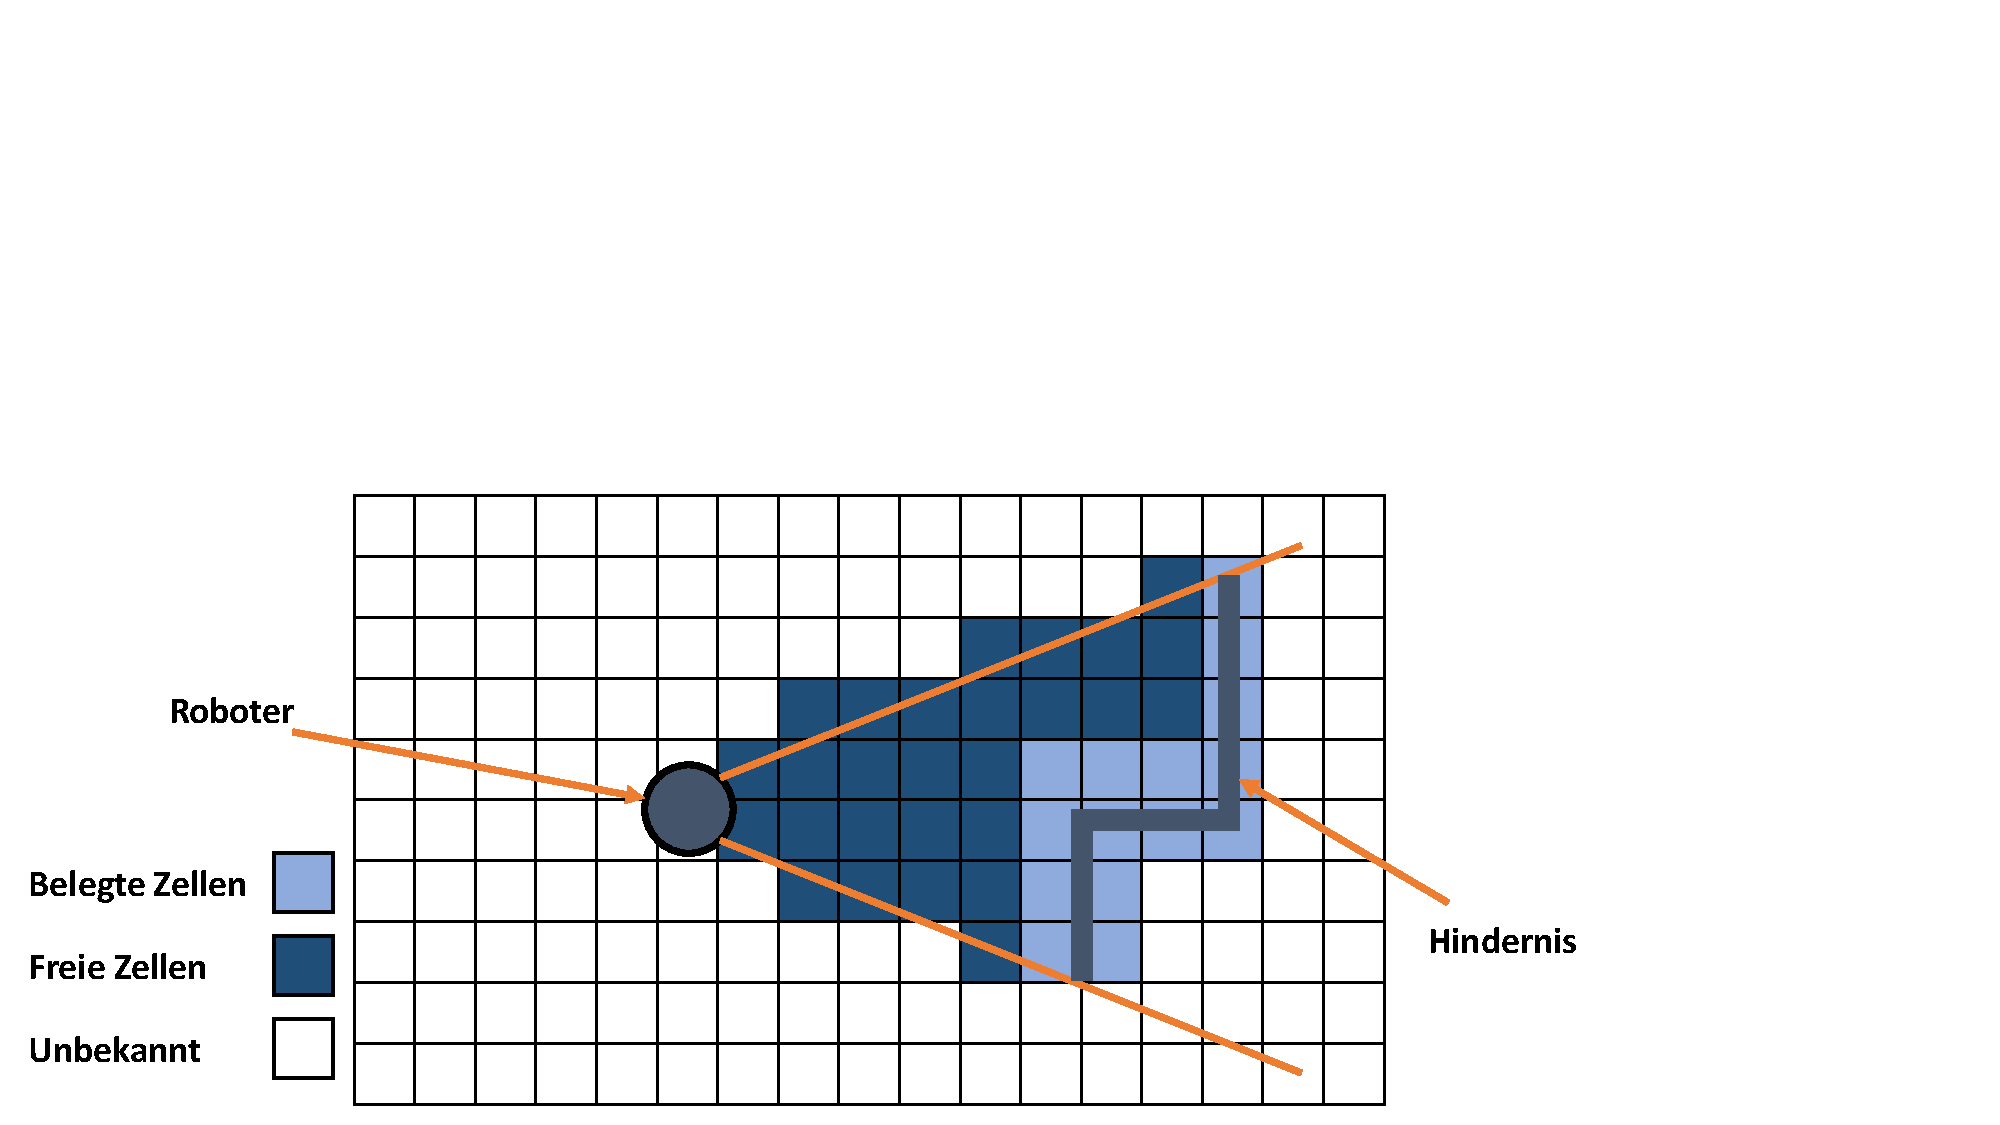
\includegraphics[width=0.7\linewidth, trim={0cm 0cm 7cm 8cm}, clip]{img/Bilder_Karten_InvSensModel_1}
\caption{Schematische Darstellung der Karten und des inversen Messmodells}
\end{figure}
Im inversen Messmodell werden nun drei Fälle unterschieden. Liegt eine Zelle außerhalb des Messkegels, kann keine Aussage über den Zustand der Zelle getroffen werden, weshalb der Wert $l_0$ zurückgegeben wird der in \ref{eq_bayes_filter_2} eingesetzt zu 
\begin{equation}
l(m_i)_t = l(m_i)_{t-1} + l_0 - l_0 = l(m_i)_{t-1}
\end{equation}
führt; die Wahrscheinlichkeit der Zelle bleibt also unverändert. 

In dem Fall, dass die Zelle innerhalb des Messkegels liegt, wird geprüft auf welchem Messstrahl und in welcher Distanz die Zelle sich befindet. Ist der Abstand zwischen der Zelle und der gemessenen Distanz kleiner als ein Toleranzmaß $\alpha$, wird angenommen, dass die Zelle belegt ist und ein entsprechender Wert $l_{\text{occupied}}$ zurückgegeben. Liegt die Zelle mehr als $\alpha$ Einheiten vor der gemessen Distanz, gilt sie als frei und das Modell liefert den Wert $l_{\text{free}}$.

\chapter{Lokaler Planer: Dynamic Window Appraoch}
Nachdem die Berechnung eines Pfades zwischen Ausgangs- und Zielposition mittels $A*$ gelöst wurde, muss als nächstes eine Folge von Steuerkommandos ermittelt werden, um den geplanten Pfad abzufahren. Den Ausgangspunkt stellt die Dynamik des roboters dar: Die Position des Roboters wird in dem Zustandsvektor 
\begin{equation}
\mVec{x}(t) = \begin{pmatrix}
x \\ y \\  \theta
\end{pmatrix}
\end{equation}
erfasst, wobei die ersten beiden Größen die Position und der Winkel $\theta$ die Blickrichtung des Roboters beschreiben. Nach wie vor gilt die Annahme, dass der Roboter in einer planen Umgebung manövriert. Die Positionsänderung wird mithilfe einer Translationsgeschwindigkeit $v$ und einer Rotationsgeschwindigkeit $\omega$ erfasst, die wiederum in dem Vektor
\begin{equation}
\mVec{u} = \begin{pmatrix}
v \\ \omega
\end{pmatrix}
\end{equation}
zusammengefasst werden. Bei den Turtlebots werden die Motoren drehzahlgeregelt, weshalb der Geschwindigkeitsvektor $\mVec{u}$ die Stellgröße zur Ansteuerung des Roboters darstellt. wird die Annahme getroffen, dass die an einem Zeitpunkt $n\cdot T\idx{a}$ eingestellt Geschwindigkeit für die folgende Abtastperiode konstant ist, kann die Positionsänderung in X- und Y-Richtung mittels der folgenden Gleichungen berechnet werden:
\begin{equation}
x\idx{n+1} = x\idx{n} + \Delta x(n)
\end{equation}
\begin{equation}
y\idx{n+1} = y\idx{n} + \Delta y(n)
\end{equation}
\begin{equation}
\Delta x(n) = \left\{ \begin{array}{ll}
\frac{v\idx{n}}{\omega\idx{n}}\cdot \left( \mSin{\theta\idx{n}}-\mSin{\theta\idx{n}+\omega\idx{n}\cdot T\idx{a}}\right) & \hspace{1cm} \forall \omega\idx{n} \neq 0 \\
v\idx{n}\cdot \mCos{\theta\idx{n}}\cdot T\idx{a} & \hspace{1cm} \forall \omega\idx{n} = 0 \end{array}\right.
\end{equation}
\begin{equation}
\Delta y(n) = \left\{ \begin{array}{ll}
-\frac{v\idx{n}}{\omega\idx{n}}\cdot \left(\mCos{\theta\idx{n}}-\mCos{\theta\idx{n}+\omega\idx{n}\cdot T\idx{a}}\right) & \hspace{1cm} \forall \omega\idx{n} \neq 0 \\
v\idx{n}\cdot \mSin{\theta\idx{n}}\cdot T\idx{a} & \forall \omega\idx{n} = 0
\end{array}\right.
\end{equation}
Aus den zeitweise konstanten Geschwindigkeiten resultiert eine Kreisbahn mit dem Radius $v\idx{n} / \omega\idx{n}$ im Falle, dass $\omega\idx{n} \neq 0$ gilt. Im Extremfall mit $\omega\idx{n} = 0$ bewegt der Roboter sich rein translativ entlang einer Geraden. Somit wird der Raum der möglichen Trajektorien auf Kreisbahnen reduziert, wodurch die Komplexität des folgenden Suchproblems drastisch reduziert wird.

Unter den obigen Annahmen soll nun ein Geschwindigkeitsvektor $\mVec{u}$ gewählt werdne, um den Roboter in Richtung eines gegebenen Zielpunktes zu fahren, der in der nähren Umgebung liegt. Im ersten Schritt wird der Versuch unternommen, den Suchraum der möglichen Geschwindigkeiten durch Nebenbedingungen weiter einzugrenzen. Sowohl für die Translations- als auch die Rotationsgeschwindigkeit bestehen Maxima, die nicht überschritten werden dürfen, woraus die Menge
\begin{equation}
V\idx{s} = \left\{ (v,\omega) \mCond v < v\idx{max} \land \omega < \omega\idx{max}\right\}
\end{equation}
resultiert. Neben den Geschwindigkeiten sind auch die Beschleunigungen beschränkt, weshalb die Menge der erreichbaren Geschwindigkeiten durch die aktuellen Geschwindigkeiten  $v\idx{a}$ und $\omega\idx{a}$, und die maximalen Beschleunigungen eingeschränkt werden.
\begin{equation}
V\idx{a} = \left\{ (v,\omega) \mCond v \in \left[v\idx{a}-\dot{v}\idx{max}\cdot T\idx{a}, v\idx{a}+\dot{v}\idx{a}\cdot T\idx{a}\right] \land \omega \in \left[\omega\idx{a}-\dot{\omega}\idx{max}\cdot T\idx{a}, \omega\idx{a}+\dot{\omega}\idx{max}\cdot T\idx{a}\right] \right\}\,.
\end{equation}
Als dritte Begrenzung des Suchraums werden Hindernisse in der Umgebung herangezogen. Jedem Geschwindigkeitsparr $(v,\omega)$ kann eine Kreisbahn zugeordnet werden, wobei die Funktion $\text{dist}(v,\omega)$ die Distanz des nächsten Hindernisses am Ende der Abtastperiode auf der zugehörigen Kreisbahn wiedergibt. Wenn nun eine maximale Verzögerung von $\dot{v}\idx{max}$ und $\dot{\omega}\idx{max}$ erreicht werden kann, folgt für die maximal erlaubte Geschwindigkeit, um vor dem Hindernis bremsen zu können:
\begin{equation}
V\idx{d} = \left\{ (v,\omega) \mCond v \leq \sqrt{2\cdot \text{dist}(v,\omega)\cdot \dot{v}\idx{max}} \land \omega \leq \sqrt{2\cdot\text{dist}(v,\omega)\cdot \dot{\omega}\idx{max}} \right\}\,.
\end{equation}
Der Raum der zulässigen Geschwindigkeiten ergibt sich aus dem Schnitt der drei Mengen
\begin{equation}
V = V\idx{s} \cap V\idx{a} \cap V\idx{d}\,.
\end{equation}
Nun gilt es eine Geschwindigkeit aus dem Suchraum $V$ auszuwählen, wofür wiederum ein Gütekriterium definiert wird, dessen Optimum erzielt werden muss. Bei der Auswahl der Zielfunktion werden drei Aspekte berücksichtigt: Der Roboter soll sich möglichst weit in Richtung des Zielpunktes bewegen, die Blickrichtung des Roboters soll am Ende der folgenden Abtastperiode auf den Zielpunkt gerichtet sein, und die Distanz zwischen dem Roboter und Hindernissen soll möglichst groß gehalten werden. Diese drei Teilziele werden jeweils durch eine separate Funktion beschrieben, deren Summe bei der Suche maximiert werden soll. Die Richtungsabweichung wird durch die Funktion
\begin{equation}
\text{heading}(v, \omega) = \pi - \varphi \hspace{1.5cm} \varphi = \sphericalangle 
\end{equation}
erfasst, wobei $\varphi$ den Winkel zwischen Blickrichtung und Zielpunkt beschreibt. Die Gewichtung der Geschwindigkeit erfolgt mittels einer simplen Gerade der Form
\begin{equation}
\text{velocity}(v, \omega) = a\cdot v\,.
\end{equation}
Um den Abstand von Hindernissen zu bewerten, wird wieder die bekannte Funktion $\text{dist}(v,\omega)$ verwendet, wobei zu beachten ist, dass im Falle einer Kurve ohne Hindernisse eine recht große Konstante zurückgeliefert wird. Zusammengeführt ergeben die einzelnen Teile die Zielfunktion
\begin{equation}
G(v, \omega) = \alpha\cdot \text{heading}(v,\omega)+ \beta\cdot \text{velocity}(v,\omega)+\gamma\cdot \text{dist}(v,\omega)\,,
\end{equation}
wobei die Faktoren $\alpha$, $\beta$ und $\gamma$ zur Normierung der Teilzielfunktionen verwendet werden. Dadurch wird sichergestellt, dass keine der drei Funktionen das Ergebnis der Optimierung überproportional beeinflusst.

\section{Anwendungsbeispiel}
Um die Funktionsprinzipien des lokalen Planers besser nachvollziehen zu können, wird an dieser Stelle schrittweise eine Implementierung erarbeitet, die anschließend in der Simulation verifiziert wird. Im ersten Schritt werden die Bedingungen für die zulässigen Geschwindigkeiten konstruiert, wofür Angaben für die maximalen Geschwindigkeiten benötigt werden. Diese werden im Datenblatt des TurtleBot \cite{TurtlebotDS} mit
\begin{equation}
v\idx{max} = 0.65 \hspace{2.5cm} \omega\idx{max} = \pi
\end{equation}
spezifiziert. Über die maximalen Verzögerung der Aktoren sagt das Datenblatt nichts aus, weshalb an dieser Stelle die Annahmen von 
\begin{equation}
\dot{v}\idx{max} = 0.65 \hspace{2.5cm} \dot{\omega}\idx{max} =  \pi 
\end{equation}
getroffen wird. Für die spätere Anwendung können die maximalen Beschleunigungen experimentell ermittelt werden und auch in der Simulation adaptiert werden. Die aktuellen Geschwindigkeiten $v\idx{a}$ und $\omega\idx{a}$ können den Odometriedaten entnommen werden, welche über die ROS-Topic \lstinline{\odom}{} veröffentlicht werden. 

Als letzte Einschränkung ist der Abstand zwischen nächstem Hindernis und dem Turtlebot zu beachten, der mithilfe der Funktion $\text{dist}(v,\omega)$ berechnet wird. Die Implementierung der Distanzfunktion macht sich wieder den Umstand zu nutzen, dass die Menge der möglichen Trajektorien begrenzt ist: Der Roboter bewegt sich auf einer Kreisbahn mit dem Radius $r=\frac{v}{\omega}$, deren Mittelpunkt $M$ simultan als Ursprung des Koordinatensystems verwendet wird. 
\begin{figure}[!ht]
\centering
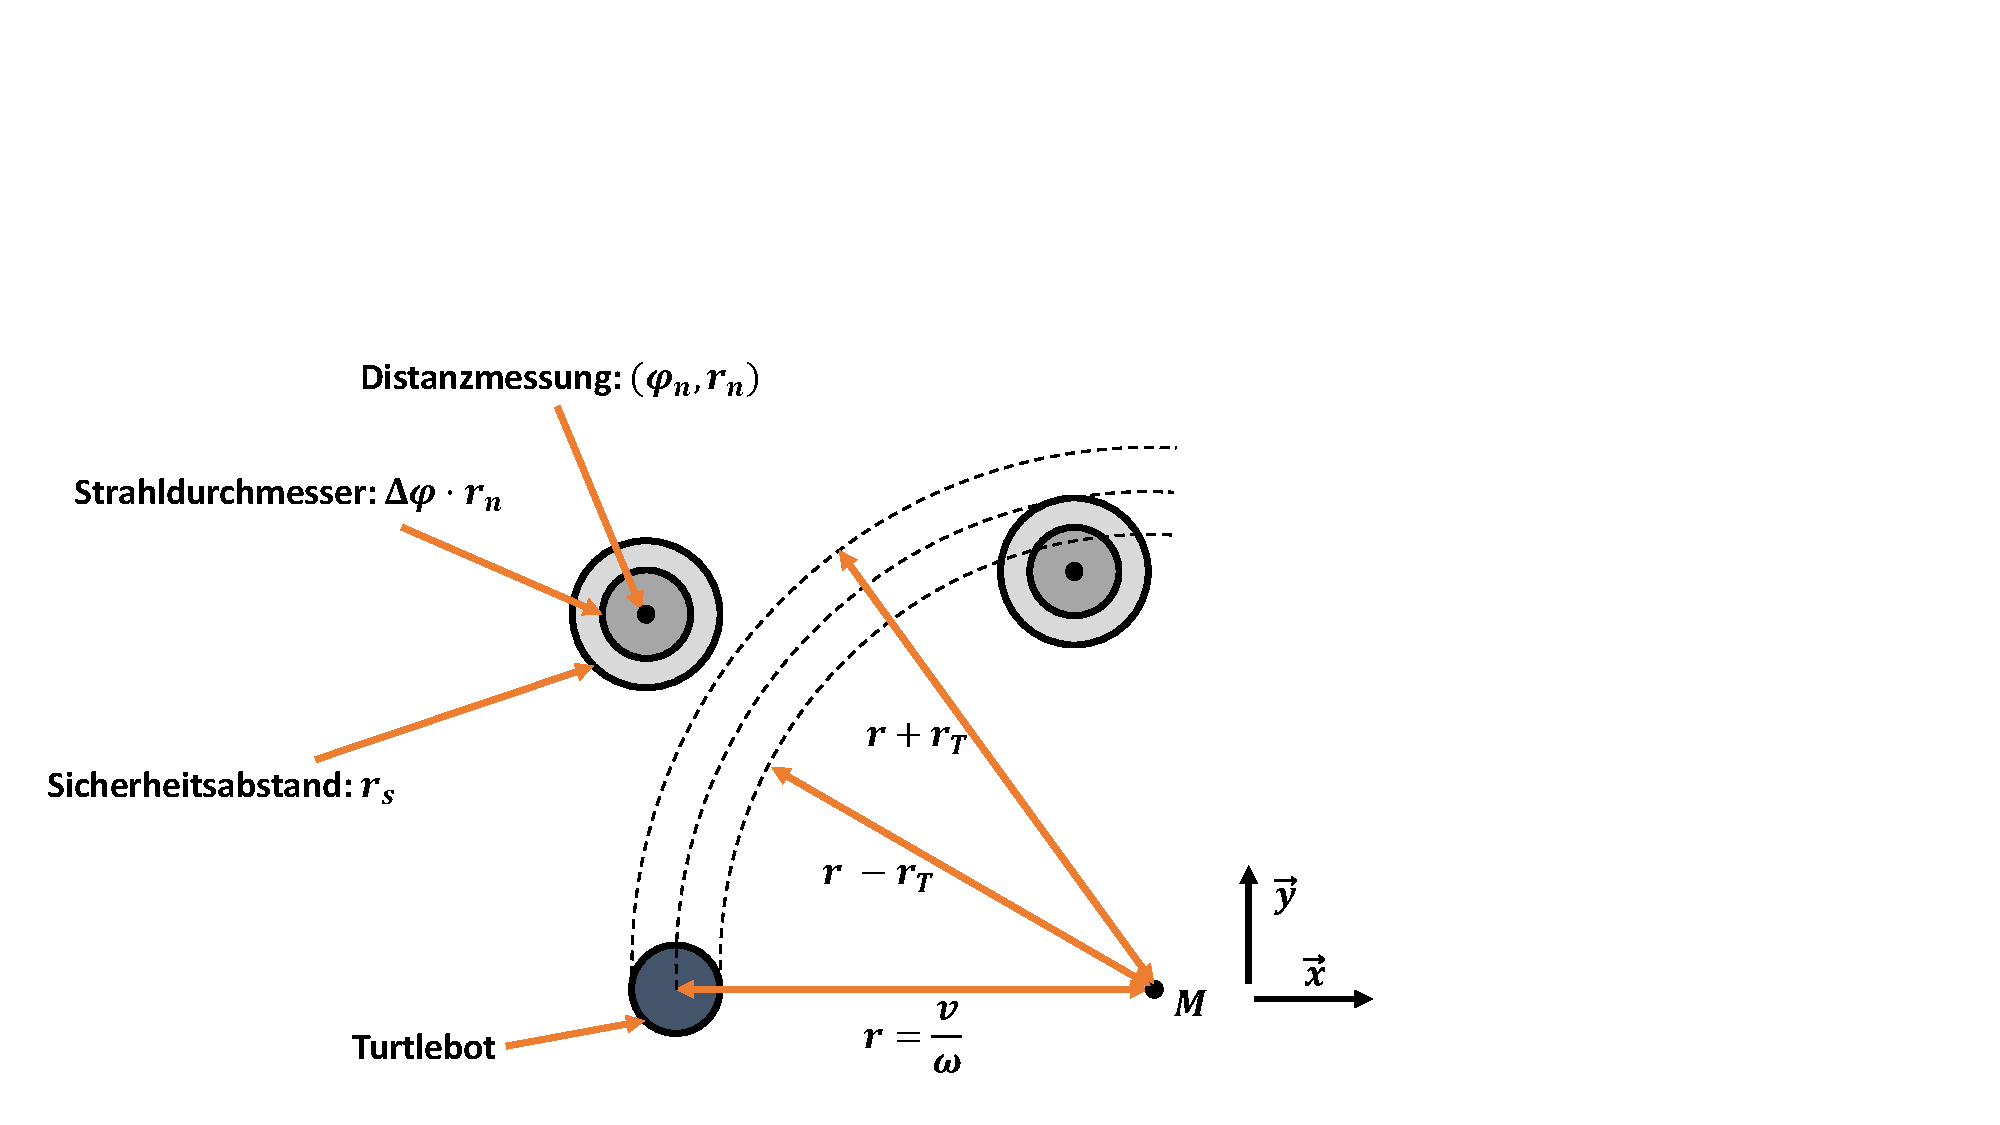
\includegraphics[width=0.7\linewidth, trim={0cm 0cm 10cm 6cm}, clip]{img/Distanz_img1}
\caption{Darstellung der Trajektorie und Hindernissen}
\end{figure}

Somit folgt für die Position des TurtleBot
\begin{equation}
\mVec{p}\idx{R} = \left\{\begin{array}{rl}
-\begin{pmatrix} r \\ 0 \end{pmatrix} & \hspace{1cm} \forall \omega < 0 \\
\begin{pmatrix} r \\ 0 \end{pmatrix} & \hspace{1cm} \forall \omega > 0 
\end{array}\right.\,,
\end{equation}
wobei der Fall $\omega = 0$ separat betrachtet werden muss. Da es sich bei dem Roboter um keinen Punkt sondern eine Kreisscheibe mit dem Radius $r\idx{R}$ handelt, wird ein Schlauch mit Innenradius $r\idx{I} = r - r\idx{R}$ und Außenradius $r\idx{A} = r + r\idx{R}$ überfahren. Diese Fläche kann in Polarkoordinaten als die Punktmenge
\begin{equation}
K\idx{R} = \left\{ (\phi, s) \mCond s \in \left[r\idx{I},r\idx{A}\right] \land \phi \in \left[0, 2\cdot \pi\right]\right\} 
\end{equation}
dargestellt werden.
Der Laserscanner liefert einen Messvektor $\mVec{z}$, dessen Element jeweils ein Paar $(\varphi\idx{n}, r\idx{n})$ sind, das sowohl den Winkel zwischen Messstrahl und Blickrichtung als auch die darauf gemessene Entfernung $r\idx{n}$ beschreibt. Folglich stellt das Paar die Position eines Messpunktes relativ zu dem TurtleBot dar, wobei die Darstellung in Form von Polarkoordinaten vorliegt. Liegt der Messpunkt zwischen den Kreisbahnen $r+r\idx{T}$ und $r-r\idx{T}$ blockiert er die Bahn des Roboters. Des Weiteren muss beachtet werden, dass eine finite Anzahlen von Messstrahlen vorliegt, weshalb jeder Messpunkt einen Messkegel mit Öffnungswinkel $2\cdot \Delta\varphi$ repräsentiert. Insofern ergibt es Sinn zu prüfen, ob der Kreis mit Mittelpunk $(\varphi\idx{n},r\idx{n})$ und Radius $\Delta\varphi\cdot r\idx{n}$ die Bahn des Roboters schneidet. Als zusätzliche Absicherung kann der Kreis um den Messpunkt um einen Sicherheitsabstand $r\idx{s}$ erweitert werden. Eine mathematische Formulierung resultiert, indem die Position des Messpunktes $\mVec{p}\idx{n}$ zunächst in dem Koordinatensystem dargestellt wird:
\begin{equation}
\mVec{p}\idx{n} = \mVec{p}\idx{R} + \begin{pmatrix} \mSin{\varphi\idx{n}} \cdot r\idx{n} \\ \mCos{\varphi\idx{n}}\cdot r\idx{n}\end{pmatrix}\,.
\end{equation}
Die im Kreis enthaltene Menge ergibt sich aus allen Punkten, deren Abstand zu dem Messpunkt kleiner als der Radius ist:
\begin{equation}
K\idx{M} = \left\{ \mVec{p} \mCond \mNorm{\mVec{p}-\mVec{p}\idx{n}} \leq \Delta\varphi\cdot r\idx{n} + r\idx{s}\right\}\,.
\end{equation}
Somit kann formal geprüft werden, ob das in einer Messung $(\varphi\idx{n},r\idx{n})$ identifizierte Hindernis auf einer durch das Geschwindigkeitspaar $(v,\omega)$ definierten Kreisbahn liegt. Ergibt der Schnitt der Mengen
\begin{equation}
K\idx{R} \cap K\idx{M}
\end{equation}
die leere Menge $\emptyset$, so wird die Trajektorie nicht von dem Hindernis blockiert. Allerdings stellt die Berechnung der Schnittmenge kein elegantes Verfahren dar, um die Position des Hindernisses zu prüfen. An dieser Stelle bietet es sich an, den Abstand $d$ eines Messpunktes $\mVec{p}\idx{n}$ zu dem Ursprung $M$ zu berechnen;
\begin{equation}
d = \mNorm{\mVec{p}\idx{n}}\,.
\end{equation}
Alle Punkte des Messkreises $K\idx{M}$ liegen zwischen dem maximalen Abstand
\begin{equation}
d\idx{max} = d + \Delta\varphi\cdot r\idx{n} + r\idx{s}
\end{equation}
und dem minimalen Abstand
\begin{equation}
d\idx{min} = d - \Delta\varphi\cdot r\idx{n} - r\idx{s}\,,
\end{equation}
wodurch sich die Prüfung auf eine simple Fallunterscheidung reduziert. Liegt einer der Abstände $d\idx{max}$ und $d\idx{min}$ zwischen den Radien $r\idx{A}$ und $r\idx{I}$, so blockiert das Hindernis die Kreisbahn. Das selbe Resultat ergibt sich in dem Fall, dass sowohl $d\idx{max} > r\idx{A}$ als auch $d\idx{min} < r\idx{I}$ gilt. Liegt ein Hindernis auf der Bahnkurve, so entspricht dessen Winkelposition $\gamma$ der Polarkoordinate des Messpunktes
\begin{equation}
\gamma = \sphericalangle \mVec{p}\idx{n}\,,
\end{equation}
woraus für die auf der Kreisbahn zurückzulegende Distanz
\begin{equation}
\text{dist}(v, \omega) = \gamma \cdot r
\end{equation}
folgt. In dem Falle einer nicht blockierten Trajektorie, gibt die Funktion die maximale Distanz zurück, die in einem Intervall passiert werden kann.
\begin{equation}
\text{dist}(v, \omega) = \left\{ \begin{array}{ll}
v\idx{max}\cdot T\idx{a} & \hspace{1cm}\forall n: K\idx{R}\cap K\idx{M} = \emptyset \\
\gamma \cdot r & \hspace{1cm}\exists n: K\idx{R}\cap K\idx{M} \neq \emptyset
\end{array}\right.\,.
\end{equation}
Somit liegen nun alle Mittel bereit, um den begrenzten Suchraum 
\begin{equation}
V = V\idx{s}\cap V\idx{a}\cap V\idx{d}
\end{equation}
zu konstruieren. Im nächsten Schritt muss die Zielfunktion
\begin{equation}
G(v, \omega) = \alpha\cdot \text{heading}(v,\omega) + \beta\cdot \text{velocity}(v,\omega) + \gamma\cdot \text{heading}(v,\omega)
\end{equation}
maximiert werden, wofür zunächst die Funktionen $\text{heading}(v,\omega)$ und $\text{velocity}(v,\omega)$ implementiert werden müssen. Letztere gibt lediglich den Geschwindigkeitswert zurück:
\begin{equation}
\text{velocity}(v,\omega) = v\,.
\end{equation}
Die Funktion $\text{heading}(v,\omega)$ gestaltet sich als etwas schwieriger, da hier der Winkel zwischen dem Zielpunkt und der Blickrichtung des Roboters berechnet werden soll. Hier stellt sich die Frage, welcher Punkt als Ziel anvisiert werden soll. Immerhin wurde bei der globalen Planung eine Folge von Positionen berechnet, die den Pfad zum letztendlichen Ziel bilden. Ein Ansatz besteht darin, den geplanten Pfad schrittweise abzuarbeiten, d.h. jeweils der erste Punkte wird angefahren. Wurde das lokal aktuelle Ziel erreicht wird der nächste Punkt des Pfades als lokales Ziel vorgegeben. Bei dieser Variante ergibt sich das Problem, dass eventuell mehrere Punkte des globalen Pfades in einem Abtastintervall erreicht werden können. Wird nun lediglich der erste anvisiert, bewegt sich der Roboter unnötig langsam. Aus diesem Grund kann ein zweiter Ansatz verfolgt werden, bei dem der Punkt des Pfades als Ziel verwendet wird, der einerseits in dem Abtastintervall erreicht werden kann, andererseits aber möglichst weit von der aktuellen Position entfernt ist. In den folgenden Simulationen werden beide Vorgehensweisen implementiert und miteinander verglichen.

Steht ein Zielpunkt fest und ist die Position des Roboters bekannt - was in der ersten Simulationsreihe angenommen wird -, so kann der Winkel $\phi$ zwischen Blickrichtung und Zielposition mithilfe simpler Trigonometrie berechnet werden. Es folgt
\begin{equation}
\text{heading}(v,\omega) = \pi - \phi\,.
\end{equation}

Zuletzt müssen die Gewichtungsfaktoren $\alpha$, $\beta$ und $\gamma$ gewählt werden. Sollen alle drei Funktionen das Optimierungsergebnis gleichermaßen beeinflussen bieten sich die Gewichtungen
\begin{equation}
\alpha = \frac{1}{\pi};\hspace{1cm} \beta = \frac{1}{v\idx{max}}; \hspace{1cm} \gamma = \frac{1}{v\idx{max}\cdot T\idx{a}}
\end{equation} 
an. Alternativ können die Ziel unterschiedlich stark in die Bewertung einfließen indem die Gewichte ungleich verteilt werden. Für die Lösung des Suchproblems bietet es sich an, den Suchraum zu diskretisieren, das heißt es werden Geschwindigkeitsinkremente $\Delta v$ und $\Delta \omega$ gewählt, woraus die Menge $G(V)$ berechnet wird. Das Optimum 
\begin{equation}
\text{arg}\text{max} G(V)
\end{equation}
kann durch einen simplen brute-force Ansatz bestimmt werden. Bei der Wahl der Abtastintervalle $\Delta v$ und $\Delta \omega$ ist ein Kompromiss zwischen Rechenaufwand und Qualität des Ergebnisses zu treffen. Dieser Einfluss wird in der anschließend Simulation weiter untersucht.

\chapter{Erprobung der Navigation}
In diesem Kapitel werden die Ergebnisse der zuvor diskutierten Algorithmen in realen Anwendungsszenarien untersucht. Als Beispiel dient der Laborraum F001 der Hochschule Karlsruhe, von dem im Voraus eine Karte mithilfe des ROS-Pakets \lstinline{hector_slam}{} aufgezeichnet wurde. An dieser Stelle werden drei verschiedene Anwendungsfälle untersucht. Im Ersten wurde der Raum im Vergleich zur Karte nicht verändert. Außerdem wird angenommen, dass die Position des Roboters zu Beginn der Navigation bekannt ist. Somit handelt es sich um den trivialsten Anwendungsfall der Navigation, womit die Grundfunktionen nachgewiesen werden sollen.
Im zweiten Szenario wird der Fall untersucht, das der auf der Karte unmittelbare Weg zum Ziel durch ein Hindernis blockiert wird, wodurch gezwungenermaßen Sensordaten beachtet werde müssen, um einen Weg zum Ziel zu planen.
Der letzte Test dient zur Beurteilung der Lokalisierung. In diesem Fall wird die Roboterposition als unbekannt angenommen und durch mittels einer ungenauen Schätzung initialisiert. 

\newpage
\section{Anwendungsszenario 1: Triviale Navigation}
Das erste Szenario dient auf der einen Seite dem Nachweis der Grundfunktionen der Navigation. Auf der anderen Seite wird das simple Beispiel genutzt, um die Bedienung und Auswertung des Experiment mittels \lstinline{RViz}{} zu erläutern. Den Ausgangspunkt aller Experimente stellt die  Karte des Labors dar, die unter Anderem in der folgenden Abbildung zu sehen ist. Die schwarzen Pixel stellen Hindernisse, die hellgrauen freie Flächen und die restlichen undefinierte Flächen dar.
\begin{figure}[!ht]
\centering
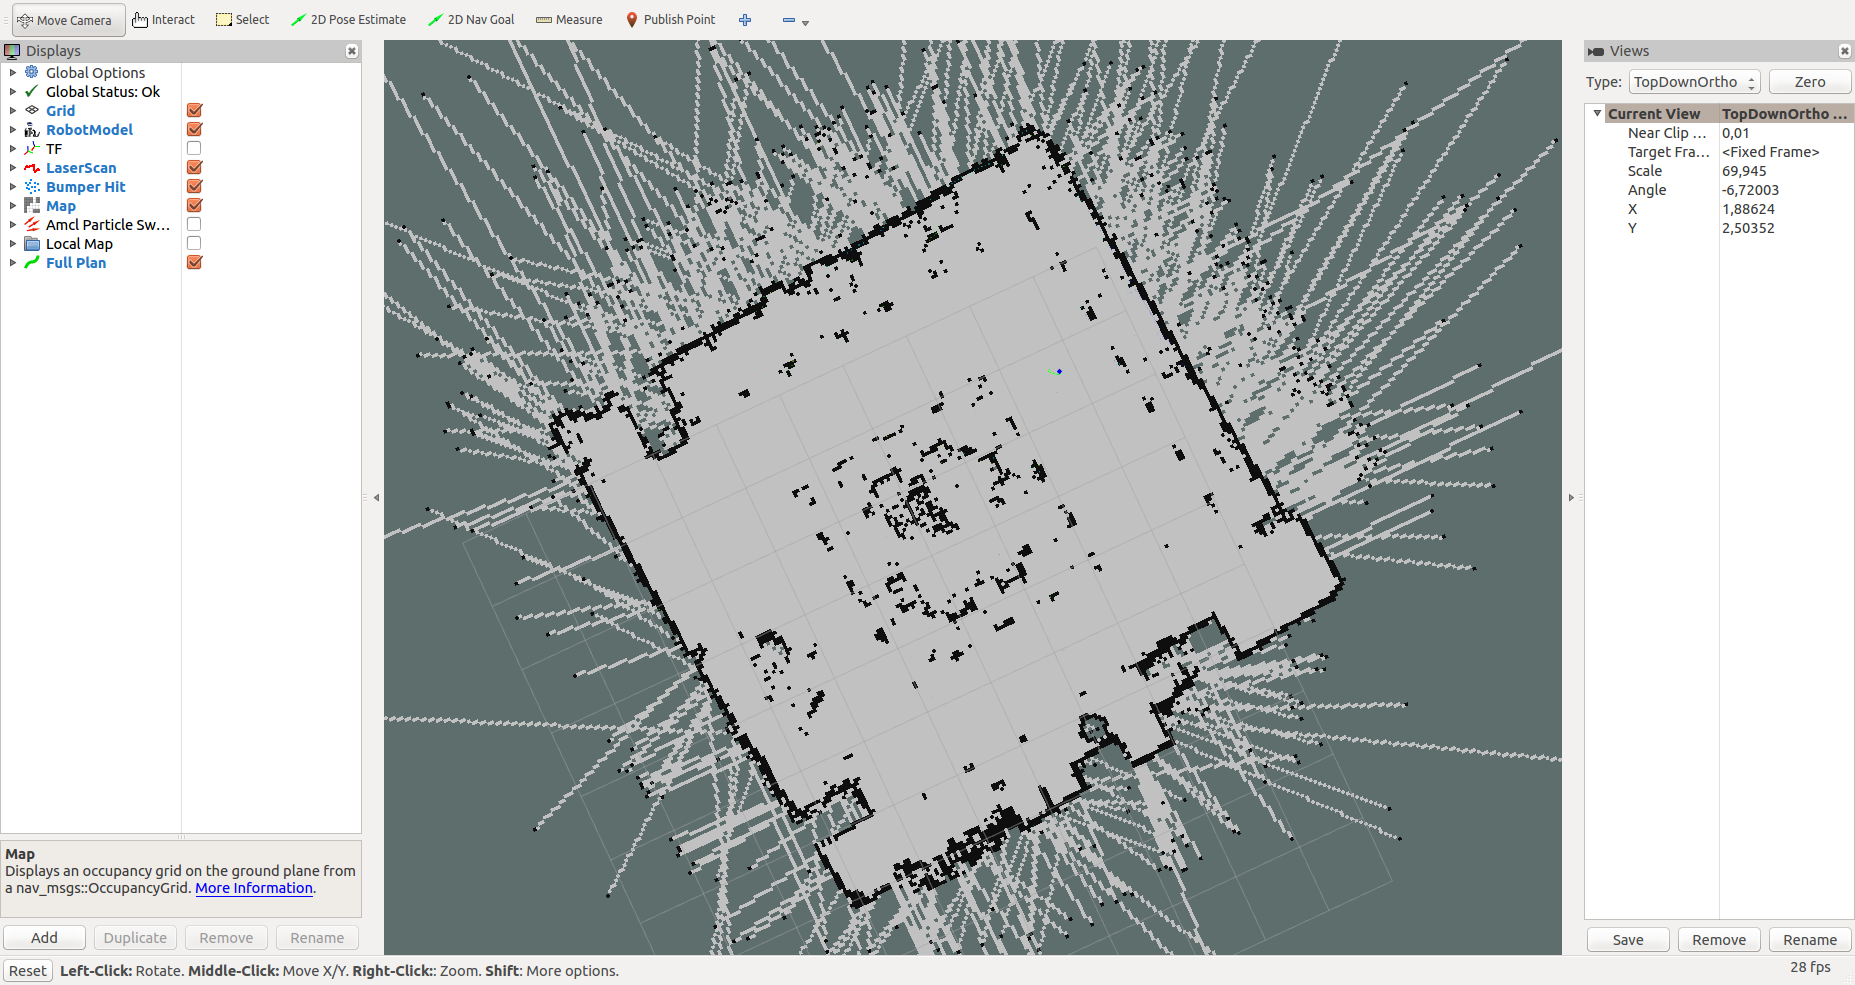
\includegraphics[width=0.8\linewidth]{img/Experiment1_RViz_Overview.png}
\caption{Übersicht von \lstinline{RViz}{}}
\end{figure}
Die Karte wird von \lstinline{RViz}{} angezeigt. Um die Visualisierung zu konfigurieren, können die Elemente auf der linken Seite nach Bedarf an- und abgewählt werden. In der Toolbar können die Elemente \lstinline{2D Pose Estimate}{} und \lstinline{2D Nav Goal}{} genutzt werden, um die eine Positionsschätzung anzugeben und das Ziel der Navigation anzugeben.
Mithilfe Letzteren wird ein Ziel in der entgegengesetzten Ecke des Raums vorgegeben, woraufhin ein globaler Pfad geplant wird, der in der folgenden Abbildung zu sehen ist.
\begin{figure}[!ht]
\centering
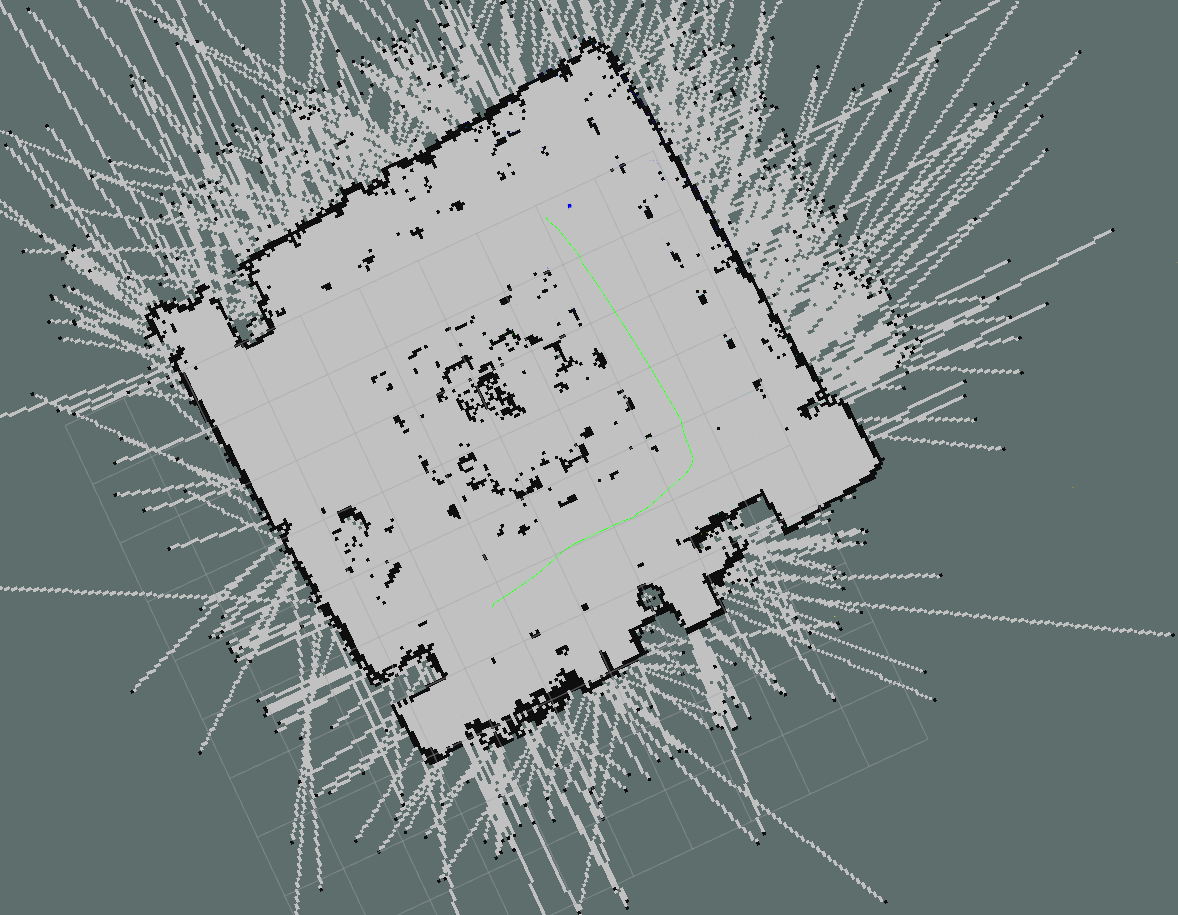
\includegraphics[scale=0.6, trim={7cm 6cm 9cm 3cm},clip]{img/Experiment1_Bild_Fullpath.png}
\caption{Globaler Plan}
\end{figure}

\newpage
Wie der oben eingezeichnete Pfad entsteht, wird recht leicht ersichtlich, wenn die globale Kostenkarte betrachtet wird. Die Bewertung der Zellen beginnt jeweils in den belegten Hindernissen und wird exponentiell fallend von diesen weg propagiert.
\begin{figure}[!ht]
\centering
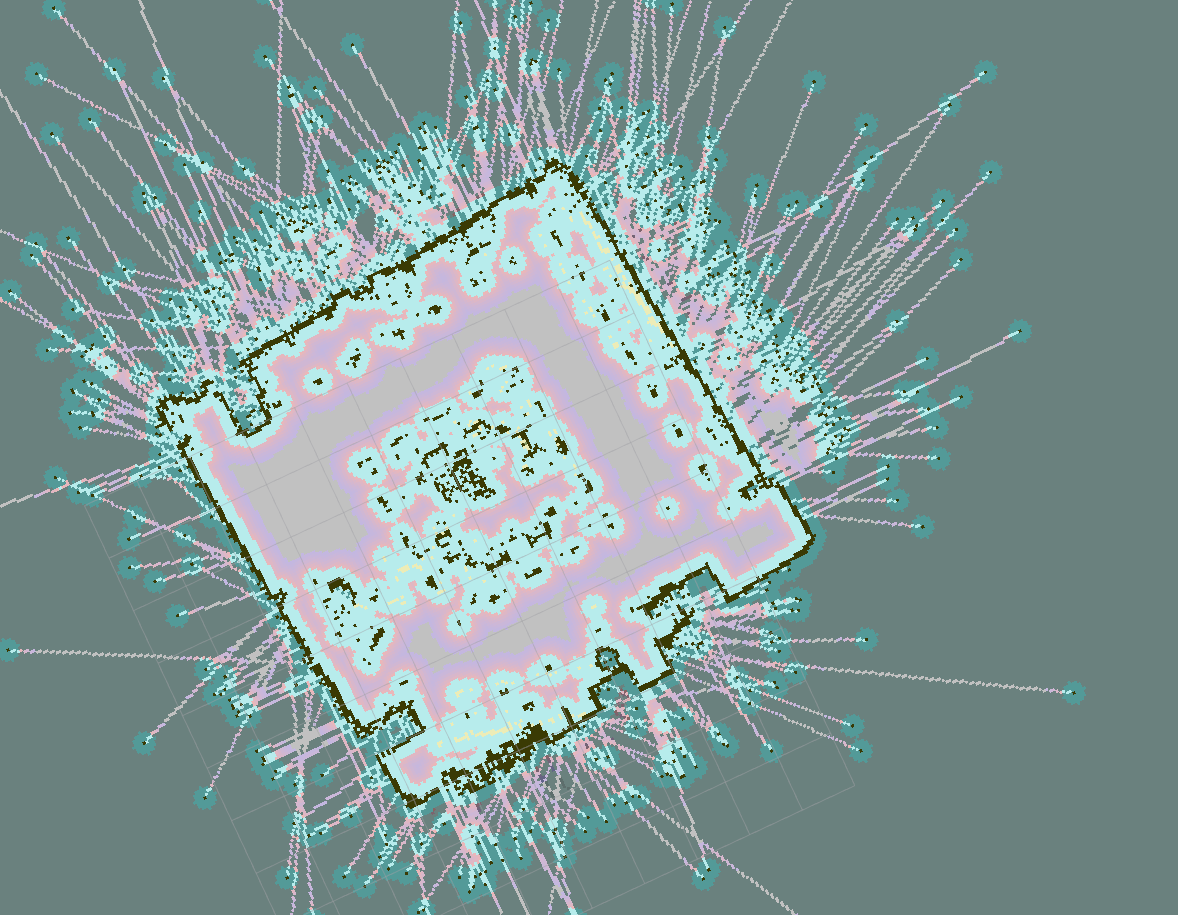
\includegraphics[scale=0.5, trim={4cm 2cm 9cm 3cm},clip]{img/Experiment1_Global_Costmap.png}
\caption{Globale Kostenkarte des Labors}
\end{figure}
Der gezeigt Pfade wurde nach der Planung problemlos von dem Roboter abgefahren, womit die Grundfunktion der Navigation nachgewiesen ist.

\newpage
\section{Anwendungsszenario 2: Hindernisdetektion}
Im nächsten Schritt wird der Fall betrachtet, dass der Weg des Roboters durch ein unbekanntes Hindernis versperrt wird. Darunter ist ein Objekt zu verstehen, dass bei der Kartenaufzeichnung nicht vorhanden war, weshalb der Roboter auf seine Sensordaten zurückgreifen muss, um den Gegenstand zu detektieren und in die Wegplanung einzuarbeiten. In der folgenden Abbildung sind die Position des Roboters als auch die aktuellen Sensordaten zu erkennen. An letzteren lässt sich die Position des Hindernisses deutlich erkennen.
\begin{figure}[!ht]
\centering
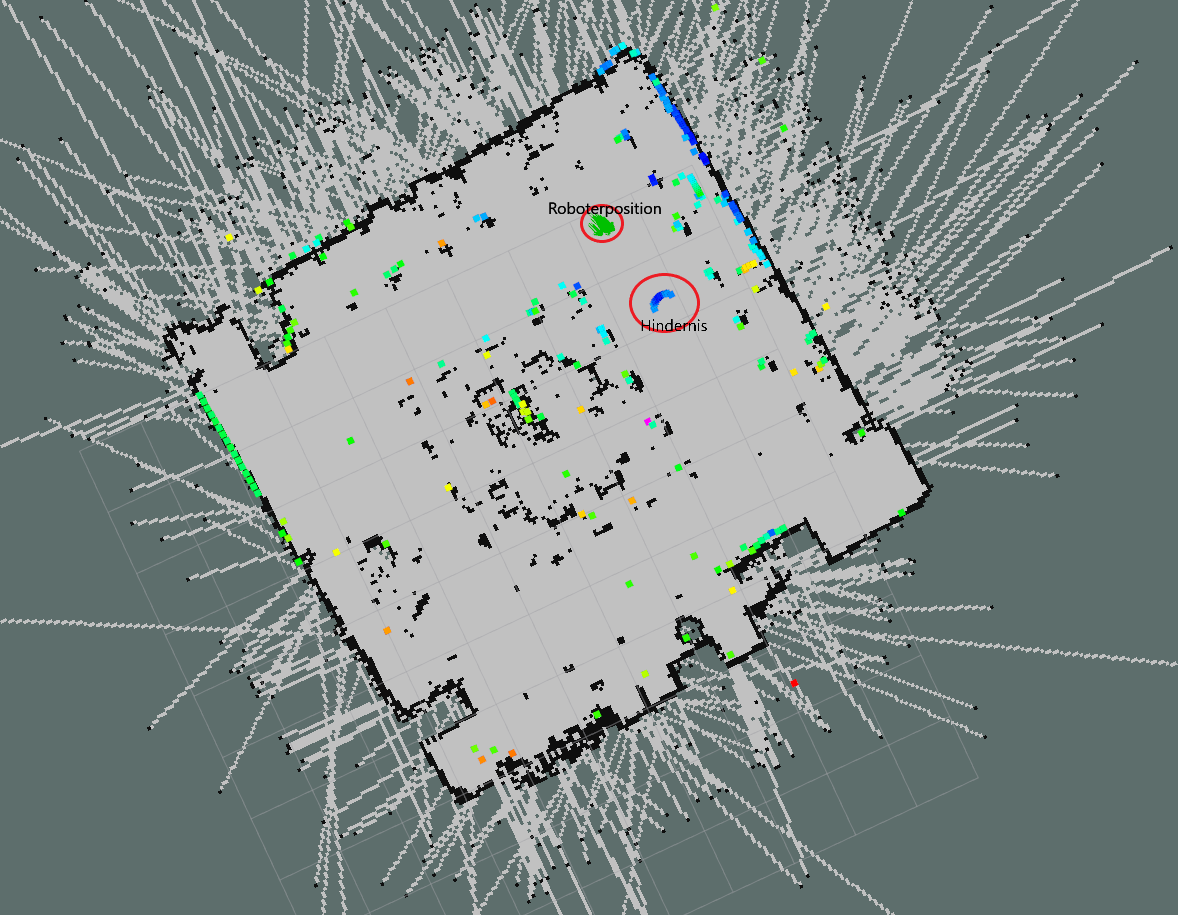
\includegraphics[scale=0.9,trim={13cm 13cm 9cm 2cm},clip]{img/Experiment2_Laserscan_Hindernis.png}
\caption{Roboter und Sensordaten mit Hindernis}
\end{figure}
\newpage
Die beiden weiteren Abbildungen zeigen wie die Sensordaten in die globale Kostenkarte integriert werden und wie daraufhin der globale Plan um die Distanzmessungen herumführt.
\begin{figure}[!ht]
\centering
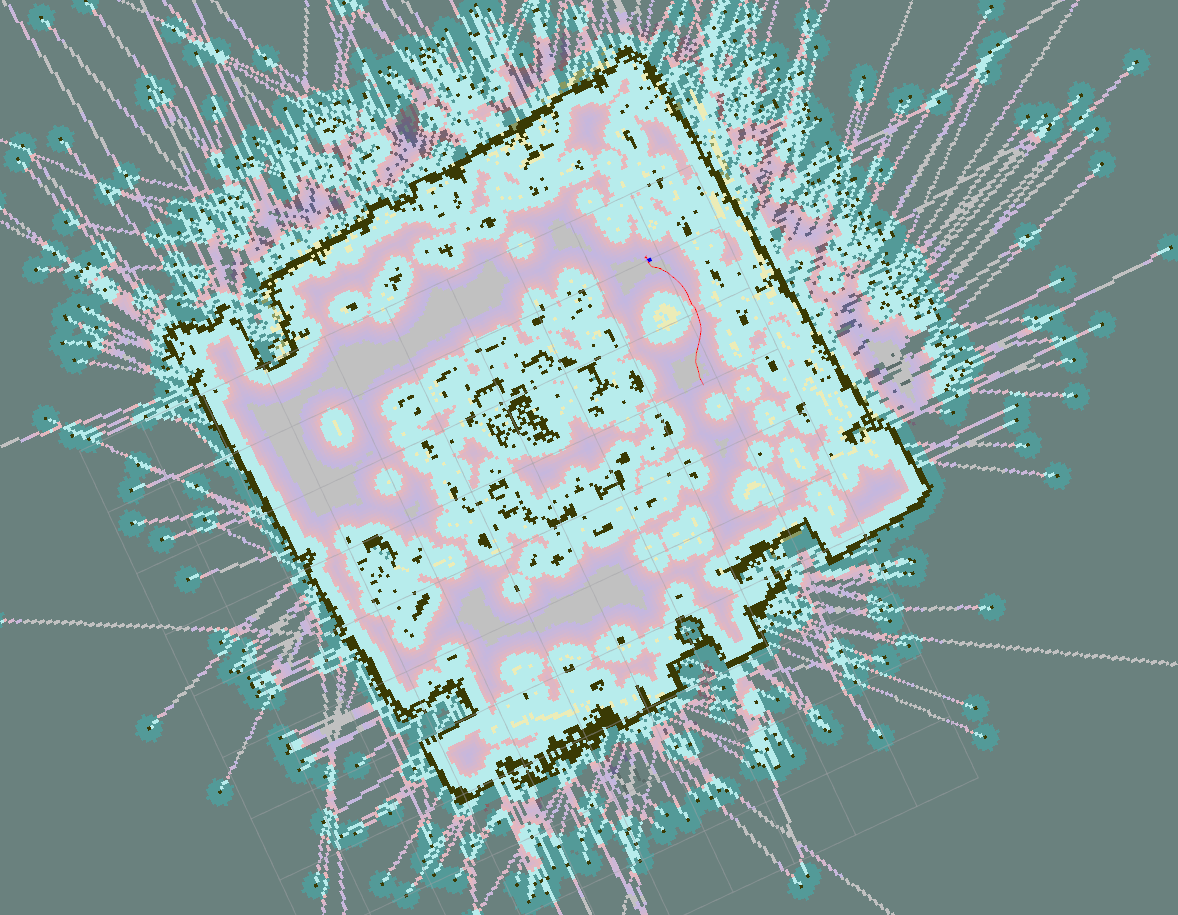
\includegraphics[width=0.45\linewidth ,trim={13cm 11cm 9cm 2cm},clip]{img/Experiment2_Global_Plan_Hindernis.png}
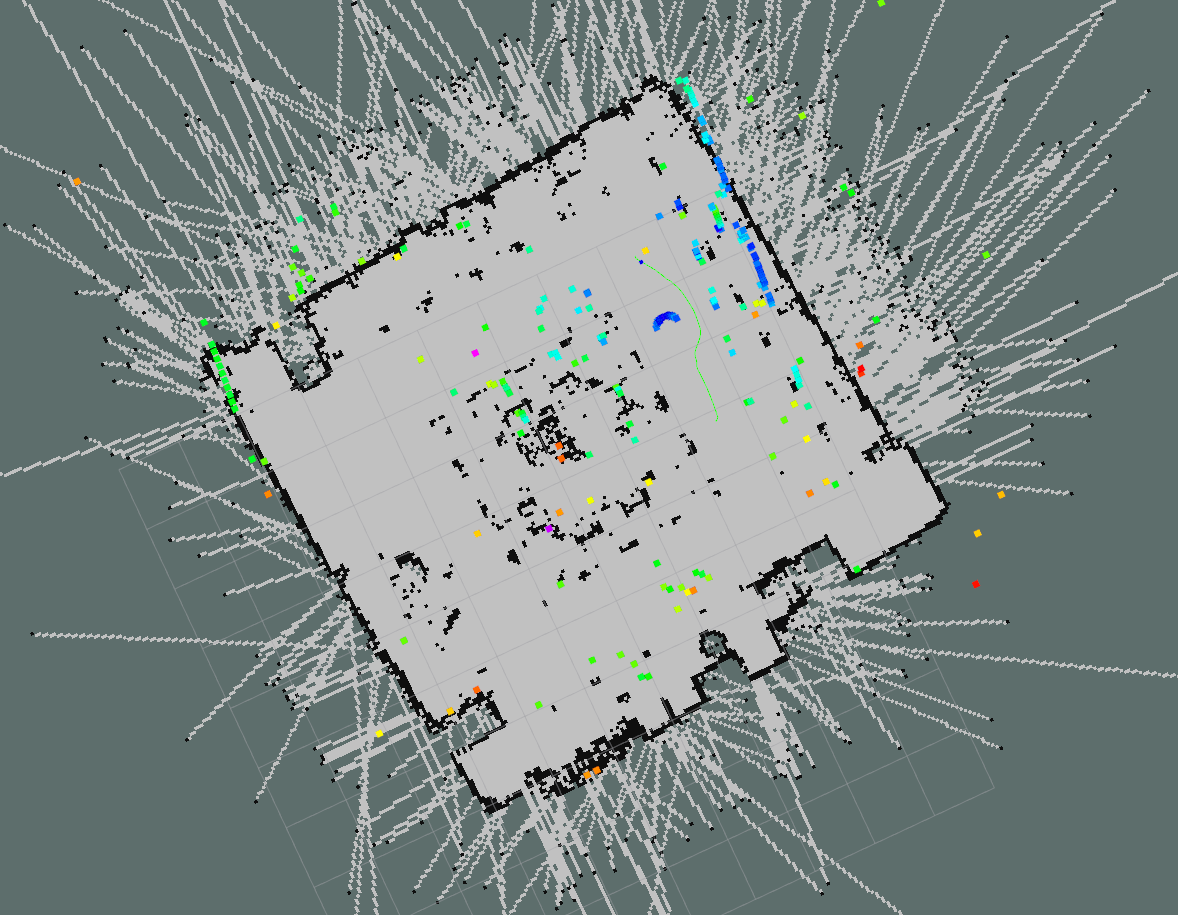
\includegraphics[width=0.45\linewidth ,trim={13cm 11cm 9cm 2cm},clip]{img/Experiment2_Global_Plan_Lascerscan_Hindernis.png}
\caption{Integration der Sensordaten in die Pfadplanung}
\end{figure}

In dem Experiment hat der Roboter das Hindernis nicht nur erfolgreich erkannt und in die Planung aufgenommen, sondern konnte die Route auch abfahren. Allerdings wurde hierbei die Geschwindigkeit deutlich reduziert, was darauf zurückzuführen ist, dass der Plan nach wie vor durch suboptimale Zonen führt. Der Grund hierfür liegt darin, das keine alternative Route zum Ziel führt, was aber auch zur Folge hat, dass der lokale Planer die Geschwindigkeit des Roboters reduziert, um auf potentielle Kollisionen reagieren zu können.

\newpage
\section{Anwendungsszenario 3: Lokalisierung}
Im letzten Versuch soll die Performanz der AMC-Lokalisierung untersucht werden. Hierfür wird der Roboter an einer Position im Raum ausgesetzt, die der Navigation nur als fehlerbehaftete, ungenaue Schätzung übergeben wird. Das Partikelfilter der Lokalisierung wird durch eine Positionsschätzung zurückgesetzt, das heißt die Partikel werden neu gezogen, wobei die geschätzte Position als Mittelwert der mehrdimensionalen Normalverteilung verwendet wird. Die initiale Varianz wird als Parameter des Algorithmus festgelegt. Die folgende Abbildung zeigt diesen Ausgangszustand, wobei die grünen Pfeile die verschiedenen Partikel darstellen, die wiederum als mögliche Positionen des Roboters verstanden werden. Außerdem sind die aktuellen Sensorwerte im Verhältnis zum Mittelwert der Partikelwolke eingezeichnet. Aus dem Vergleich der Distanzmessungen und des Wandverlaufs in der Karte wird ersichtlich, wie die Positionsschätzung des Roboters angepasst werden muss, sodass die Sensordaten mit der Umgebung übereinstimmen.
\begin{figure}[!ht]
\centering
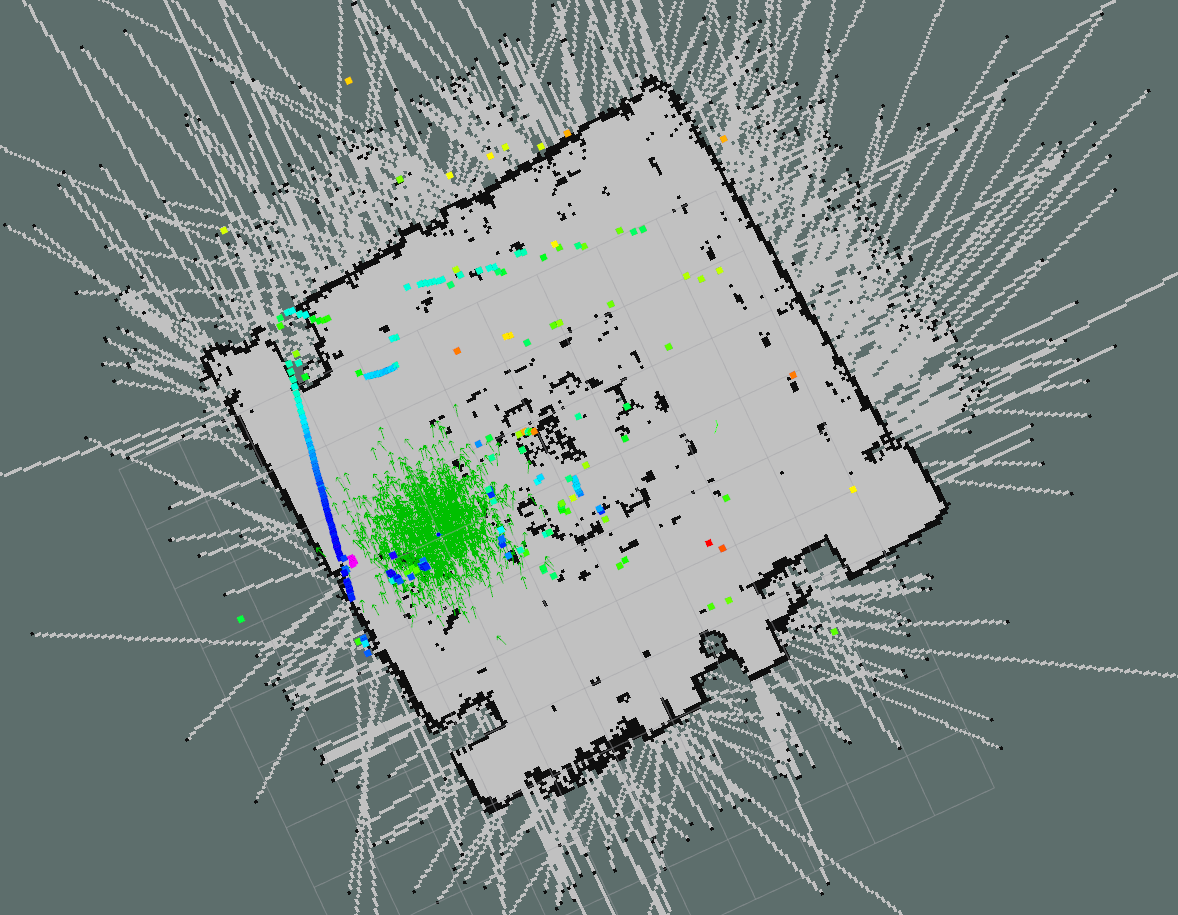
\includegraphics[width=0.7\linewidth, trim={4cm 5cm 12cm 6cm},clip]{img/Experiment3_Lokalisierung_1.png}
\caption{Ausgangszustand der Lokalisierung nach Positionsschätzung}
\end{figure}

Im nächsten Schritt der Navigation ein Zielpunkt in kurzer Distanz unmittelbar vor dem Roboter vorgegeben, woraufhin dieser die Bewegung startet. Während der Bewegung wird deutlich, dass sich der Mittelwert der Positionsschätzung verändert, was sich durch die Ausrichtung der Distanzmessungen zu dem Verlauf der Wände manifestiert. Dies zeigt sich in der nächsten Abbildung, wobei das Zusammenrücken der Partikel verdeutlicht, dass die Sicherheit der Lokalisierung zunimmt.
\begin{figure}[!ht]
\centering
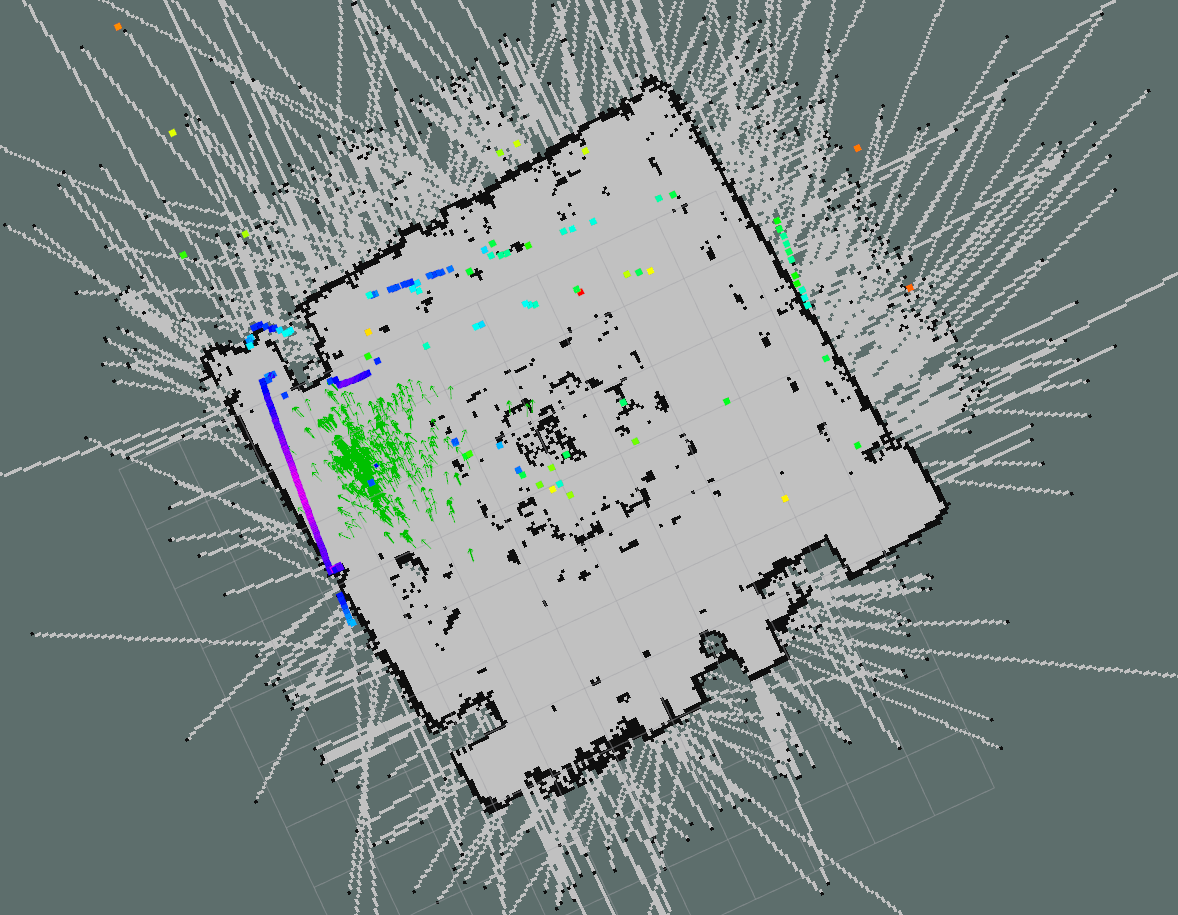
\includegraphics[width=0.7\linewidth, trim={4cm 5cm 12cm 6cm}, clip]{img/Experiment3_Lokalisierung_3.png}
\caption{Positionsschätzung nach kurzer Fahrdistanz}
\end{figure}

Die nächste Abbildung zeigt den Zustand der Lokalisierung in dem Moment, als der Zielpunkt erreicht wird. Nun stimmen die Punkte der Distanzmessung nahezu vollkommen mit den in der Karte eingezeichneten Hindernissen überein. Außerdem haben sich die Partikel weiter zusammengezogen, was für eine hohes Maß an Sicherheit der Lokalisierung spricht.
\begin{figure}[!ht]
\centering
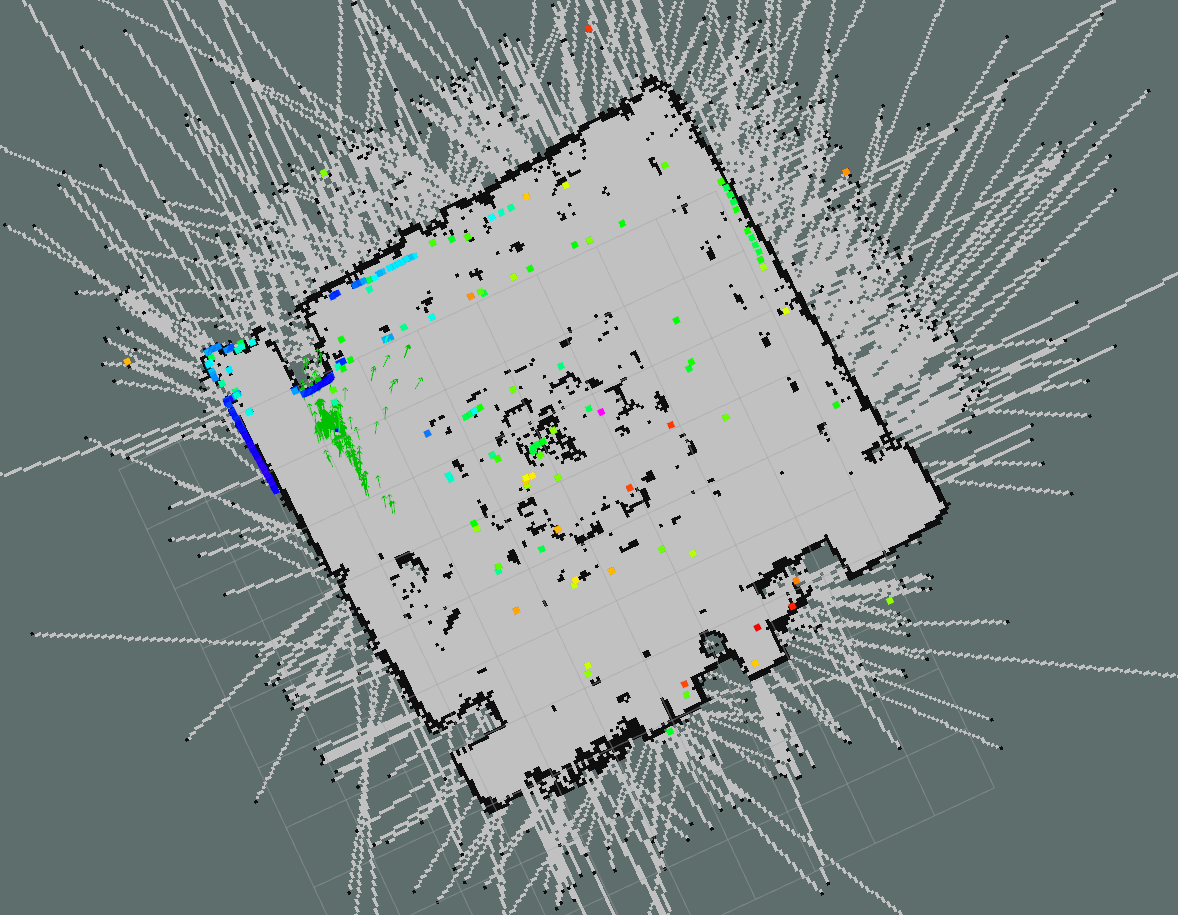
\includegraphics[width=0.7\linewidth, trim={4cm 5cm 12cm 6cm}, clip]{img/Experiment3_Lokalisierung_4.png}
\caption{Positionsschätzung bei Erreichen der Zielposition}
\end{figure}

Im letzten Schritt wird ein weiteres Navigationsziel gesetzt, woraufhin der Roboter sich weiter durch den Raum bewegt. Hier zeigt sich eine weitere Verdichtung der Partikelwolke, was sich darauf zurückführen lässt, dass die Distanzmessungen weiterhin mit der Karte übereinstimmen. Somit kann die Lokalisierung mit einem erhöhten Maß an Sicherheit als richtig angenommen werden.

An dieser Stelle sei eine negative Kopplung der Navigation und Lokalisierung erwähnt. Im Fall, dass die Lokalisierung in Form einer Positionsschätzung reinitialisiert wird und nur eine kurz entferntes Ziel angesteuert wird, wird während der Navigation die Position des Roboters durch den Lokalisierungsalgorithmus angepasst. Dies hat wiederum zur Folge, dass der Plan des Roboters überarbeitet werden muss, da die ursprüngliche Position verworfen wurde. Dies hat zur Folge, dass der Roboter wiederholte Rotationsmanöver ausführt, die von kurzen Translationsbewegung gefolgt werden. In diesem Muster bewegt sich der Roboter mehrere Male auf der Stelle, bis die Lokalisierung ein ausreichend hohes Maß an Sicherheit erreicht hat, sodass die geschätzte Position sich nur noch in einer für die Navigation nicht relevanten Größenordnung ändert.

\chapter{ROS Implementierung}
Nachdem in den vorherigen Kapiteln die theoretischen Grundlagen der Navigationsalgorithmen erläutert wurden, widmet sich dieser Teil der Arbeit der Umsetzung der Konzepte in ROS. Zunächst wird der Aufbau des Systems, Anordnung der Rechner und die Netzwerkkonfiguration betrachtet. Im Anschluss werden die Roboter schrittweise in Betrieb genommen, wobei die relevanten Dateien erklärt werden und  ein Schritt für Schritt Anleitung gezeigt wird.

Als erste Demonstration wird die Fernsteuerung der Roboter betrachtet, wofür eine Launch-Datei zur Initialisierung der Turtlebots angelegt wird. Außerdem wird auf dem Master eine Anwendung ausgeführt, um den Roboter per Tastatur zu steuern.
Im nächsten Schritt wird die Kartenaufzeichnung implementiert. Hier wird auf dem Master-PC zusätzlich das Paket \lstinline{hector_mapping}{} ausgeführt, welches die Karte erstellt. Außerdem wird \lstinline{Rviz}{} verwendet, um die aktuelle Karte und Roboterposition zu visualisieren.
Im dritten Anwendungsbeispiel wird die zuvor aufgezeichnete Karte für die autonome Navigation genutzt. Hierfür wird auf Seite des Master die vollständigen Navigationsalgorithmen konfiguriert und ausgeführt. Außerdem zeigt \lstinline{Rviz}{} in diesem Beispiel nicht nur die Karte und den Roboter an, sondern dient auch als Eingabemöglichkeit für die Zielposition.

Im Anschluss wird der Endszenario diskutiert, in dem zwei Robotern simultan navigieren. Hier entsteht auf ROS-Seite das Problem, dass Konflikte in der Namensgebung von Nachrichten und Topics entstehen. Eine mögliche Lösung stellen die unter ROS verfügbaren Namensräume dar, wodurch die Daten der beiden Roboter entkoppelt werden können. Allerdings sind in der Umsetzung dieses Lösungsansatzes Probleme mit der Lokalisierung aufgetreten, die bisher noch nicht erklärt bzw. gelöst werden konnten. An dieser Stelle wird der Fehlerfall aufgezeigt und mögliche Lösungen analysiert.

\newpage
\section{Systemstruktur}
\pdfcomment{Formulierung, die Erklärung von Master/Slave ist schlecht}
In dieser Arbeit wird die Navigation von maximal zwei Robotern zur selben Zeit betrachtet. Jeder der Roboter ist mit einem PC ausgestattet, die über WLAN mit einem TP-Link-Router verbunden sind, der als Access-Point des Netzwerks fungiert. Der Roboterverbund ist nach einem Master-Slave-Prinzip konzipiert, wobei die Roboter bzw. deren PCs als Slave agieren. Ein weiterer PC ist mit dem Router verbunden und agiert als Master. Der Master-PC ist zusätzlich mit Tastatur, Maus und Bildschirm ausgestattet und stellt somit die Steuereinheit des Systems dar. Daher stammt auch die Bezeichnung Master-PC, da von diesem die Befehlskette bedient wird. Die Slave-PCs, welche sich auf den Robotern befinden, nehmen die Befehle entgegen, arbeiten also als Slaves \pdfcomment{really?}.

Das Netzwerk läuft in dem IP-Adressbereich 192.168.0.X, wobei die Adressen des Master- und der Slave-PCs statisch zugewiesen werden. Der Master-PC ist unter der Adresse 192.168.0.100 erreichbar; Roboter R2 unter der Adresse 192.168.0.102; Roboter R4 unter der Adresse 192.168.0.104. Außerdem ist es möglich, dass sich weitere Rechner mit dem Netzwerk verbinden, wodurch auf sämtliche Daten des ROS-Netzes zugegriffen werden kann. Somit können auch Entwicklungswerkzeuge wie MATLAB verwendet werden, um die Daten abzugreifen und weiterzuverarbeiten.

Das Netzwerk trägt den Namen \lstinline{EML_Turtlebot_NET}{} mit dem Passwort \lstinline{turtlebot}{}. Die statische Konfiguration der IP-Adressen kann im Detail in \cite[S. 23]{Turtleboys} nachgelesen werden.
Auf jedem der Rechner existiert ein Nutzer mit dem Namen \lstinline{turtlebot}{} und Passwort \lstinline{turtlebot}{}, der genutzt werden kann, um eine ssh-Verbindung aufzubauen.

\newpage
\section{Inbetriebnahme der Turtlebots}
In diesem Teil der Arbeit wird die praktische Umsetzung der Navigationsalgorithmen diskutiert, wofür ROS verwendet wird. Unter ROS werden so genannte Launch-Dateien genutzt, um die beteiligten Pakete zu parametrisieren und zu starten. Typischerweise werden in jedem ROS-Projekt mehrere Launch-Dateien angelegt, die für die jeweiligen Anwendungsfälle ausgelegt sind. In dieser Arbeit werden zwei verschiedene Projekte angelegt. Auf dem Master-PC wird das Projekt \lstinline{EML_Navigation_Master}{} genutzt; auf den Slave-PCs das Projekt \lstinline{EML_Navigation_Slave}{}. Die Projektordner sind jeweils auf den Desktops der PCs zu finden. In dem Master-Projekt werden die vier Launch-Dateien
\begin{itemize}
\item \lstinline{EML_Mapping_Master.launch}{}
\item \lstinline{EML_Navigation_Master.launch}{}
\item \lstinline{EML_Navigation_Robot2_Master.launch}{}
\item \lstinline{EML_Navigation_Robot4_Master.launch}{}
\end{itemize}
genutzt, wobei die erste für die Kartenerstellung, die zweite für die Navigation eines einzelnen Roboters und die beiden letzten für die simultane Navigation der beiden Roboter verwendet werden.

In den Slave-Projekten sind die fünf Launch-Dateien
\begin{itemize}
\item \lstinline{EML_Hardware_Init_Slave.launch}{}
\item \lstinline{EML_Mapping_Slave.launch}{}
\item \lstinline{EML_Navigation_Slave.launch}{}
\item \lstinline{EML_Navigation_Robot2_Slave.launch}{}
\item \lstinline{EML_Navigation_Robot4_Slave.launch}{}
\end{itemize}
zu finden. Die Erste führt die Initialiserung der vorhandenen Hardware durch. Die vier weiteren Dateien stellen das Pendant zu den oben beschriebenen Master-Dateien dar.

\newpage
\subsection{Fernsteuerung eines Turtlebots}
Im aller ersten Schritt werden die beiden Roboter in Betrieb genommen, wofür die Fernsteuerung der beiden Geräte als Demonstration dienen soll. Auf den Slaves wird dafür die Launch-Datei \lstinline{EML_Hardware_Init_Slave.launch}{} angelegt, die die vorhandene Hardware initialisiert, sodass der Roboter über die entsprechenden ROS-Nachrichten bewegt werden kann.
\begin{lstlisting}[caption={EML\_Hardware\_Init\_Slave.launch},captionpos=b]
<launch>
	<!-- Basis-Initialisierung -->
	<include file="$(find turtlebot_bringup)/ ...
			launch/minimal.launch"/>
	
	<!-- Initialisierung des SICK-TIM551 -->
	<param name="robot_description" command="$(find xacro)/ ...
			xacro.py '$(find sick_tim)/urdf/example.urdf.xacro'"/>
	<include file="$(find turtlebot_chor_navigation)/launch/ ...
			include/sick_tim551_2050001_timefix.launch"/>
</launch>
\end{lstlisting}
In der Launch-Datei wrid zunächst eine Basisinitialisierung durchgeführt, wofür die Datei \lstinline{minimal.launch}{} aus dem offiziellem ROS-Packet \lstinline{turtlebot_bringup}{}\cite{WikiTurtlebotBringup} inkludiert wird. Als Zweites wird mithilfe einer der Launch-Datei \lstinline{sick_tim_551_2050001_} \lstinline{timefix.launch}{} aus dem Vorgängerprojekt \cite{Turtleboys} der SICK-Laserscanner initialisiert.

Um den Turtelbot über den Master-PC zu steuern, wird die Launch-Datei auf dem Slave ausgeführt.
\begin{lstlisting}[language=bash]
roslaunch EML_Navigation_Slave EML_Hardware_Init_Slave.launch
\end{lstlisting}
Die Eingabe der Steuerbefehle erfolgt auf dem Master-PC, wofür auf das Paket \lstinline{turtle}{} \lstinline{bot_teleop}{} \cite{WikiTurtlebotTeleop} zurückgegriffen wird. Zum Start wird der Befehl
\begin{lstlisting}
roslaunch turtlebot_teleop keyboard_teleop.launch
\end{lstlisting}
auf dem Master-PC ausgeführt. Daraufhin kann der Roboter mittels der Tastatur bewegt werden.

\newpage
\subsection{Aufzeichnung einer Karte}
Im nächsten Schritt wird die Kartographierung der Umgebung betrachtet, wobei die Ergebnisse der Vorgängerarbeit \cite[S. 47, ff]{Turtleboys} verwendet werden können. Auf Slave-Seite wird die Launch-Datei \lstinline{EML_Mapping_Slave.launch}{} verwendet, in zunächst die bereits angesprochene Datei zur Hardware-Initialisierung inkludiert wird. Im Anschluss werden die Launch-Dateien für die Kartenaufzeichnung des Pakets \lstinline{hector_mapping}{} \cite{WikiHector} eingebunden.
\begin{lstlisting}[caption={EML\_Mapping\_Slave.launch},captionpos=b]
<launch>
	<!-- Hardware-Initialisierung -->
	<include file="$(find EML_Navigation_Slave)/launch/ ... 
			EML_Hardware_Init_Slave.launch" />

	<!-- Hector-Mapping -->
	<node name="hector_mapping" pkg="hector_mapping" ...
			type="hector_mapping" output="screen">
        	<param name="base_frame" value="base_link"/>
        	<param name="odom_frame" value="base_link"/>
	        <param name="map_resolution" value="0.05"/>
	        <param name="map_size" value="2048"/>
	        <param name="map_start_x" value="0.5"/>
        	<param name="map_start_y" value="0.5"/>
	        <param name="map_update_distance_thresh" value="0.4"/>
	        <param name="map_update_angle_thresh" value="0.02"/>
	        <param name="map_pub_period" value="0.05"/>
	        <param name="map_multi_res_levels" value="2"/>
	        <param name="update_factor_free" value="0.4"/>
	        <param name="update_factor_occupied" value="0.9"/>
	        <param name="laser_min_dist" value="0.4"/>
	        <param name="laser_max_dist" value="10"/>
	        <param name="laser_z_min_value" value="-1.0"/>
	        <param name="laser_z_max_value" value="1.0"/>
	        <param name="pub_map_odom_transform" value="true"/>
	        <param name="output_timing" value="false"/>
	        <param name="scan_subscriber_queue_size" value="1"/>
	        <param name="pub_map_scanmatch_transform" ...
	        		value="true"/>
	        <param name="pub_map_scanmatch_transform" ...
	        		value="true"/>
	        <param name="tf_map_scanmatch_transform_ ...
	        		frame_name" value="scanmatcher_frame"/>
	    </node>
    <include file="$(find hector_geotiff)/launch/ ...
    		geotiff_mapper.launch"> </include>
    <node pkg="tf" type="static_transform_publisher" ...
    		name="map_nav_broadcaster" args="0.12 0 0 0 0 0 ...
    		base_link laser 100"/>
</launch>
\end{lstlisting}
Auf dem Master wird die Launch-Datei \lstinline{EML_Mapping_Master.launch}{} verwendet, die inhaltlich ebenfalls aus dem Vorgängerprojekt \cite{Turtleboys} übernommen ist. In der Datei wird lediglich \lstinline{Rviz}{} gestartet, um die Ergebnisse der Kartenerstellung zu visualisieren.
\begin{lstlisting}[caption={EML\_Mapping\_Master.launch},captionpos=b]
<launch>
	<!-- Starte Rviz, um Karte anzuzeigen. -->
	<param name="robot_description" command="$(find xacro)/ ...
			xacro.py '$(find sick_tim)/urdf/example.urdf.xacro'" />
	<node pkg="rviz" type="rviz" name="rviz" args="-d $(find ...
			turtlebot_chor_navigation)/rviz_cfg/rviz_sick.rviz"/>
</launch>
\end{lstlisting}
Neben den beiden Launch-Dateien muss wieder eine Anwendung zur Steuerung des Turtlebots gestartet werden. Außerdem muss am Ende der Kartenaufzeichnung die Applikation \lstinline{map_server}{} ausgeführt werden, um die Karte abzuspeichern. Es ergibt sich die folgende Anleitung für die Kartenaufzeichnung. Die einzelnen Schritten sind in \cite[S. 47 ff]{Turtleboys} ausführlich beschrieben.
\begin{lstlisting}[caption={Anleitung zur Kartenaufzeichnung},captionpos=b]
[M] roscore
[S] roslaunch EML_Navigation_Slave  EML_Mapping_Slave.launch
[M] roslaunch EML_Navigation_Master EMl_Mapping_Master.launch
[M] roslaunch turtelbot_teleop keyboard_teleop.launch
[M] rosrun map_server map_saver
\end{lstlisting}

\newpage
\subsection{Navigation eines einzelnen Roboters}
Nachdem eine Karte der Umgebung erstellt wurde, kann diese für die Navigation eines Roboters herangezogen werden. Auf dem Slave wurde dafür die Launch-Datei \lstinline{EML_Navigation_Slave.launch}{} angelegt, die lediglich eine Hardware-Initialisierung durchführt.
\begin{lstlisting}[caption={EML\_Navigation\_Slave.launch},captionpos=b]
<launch>
	<include file="$(find EML_Navigation_Slave)/launch/ ...
			EML_Hardware_Init_Slave.launch" />
</launch>
\end{lstlisting}
Auf dem Master wird die Launch-Datei \lstinline{EML_Navigation_Master.launch}{} verwendet, in der sämtliche Algorithmen der Navigation parametrisiert und gestartet werden.
\begin{lstlisting}[caption={EML\_Navigation\_Master.launch},captionpos=b]
<launch>
	<!-- Map-Server -->
	<arg name="map_file" default="$(find EML_Navigation_Master)...
			/maps/test_map.yaml"/>
	<node name="map_server" pkg="map_server" type="map_server" ...
			args="$(arg map_file)"/>
	<!-- AMC-Localization -->
	<arg name="3d_sensor" default="$(env TURTLEBOT_3D_SENSOR)"/>
	<arg name="initial_pose_x" default="0.0"/>
	<arg name="initial_pose_y" default="0.0"/>
	<arg name="initial_pose_a" default="0.0"/>
	<arg name="custom_amcl_launch_file" default="$(find ...
			turtlebot_navigation)/launch/includes/amcl/$...
			(arg 3d_sensor)_amcl.launch.xml"/>
	<include file="$(arg custom_amcl_launch_file)">
		<arg name="initial_pose_x" ...
				value="$(arg initial_pose_x)"/>
		<arg name="initial_pose_y" ...
				value="$(arg initial_pose_y)"/>
		<arg name="initial_pose_a" ...
				value="$(arg initial_pose_a)"/>
		<arg name="odom_frame_id" value="odom"/>
		<arg name="base_frame_id" value="base_footprint"/>
		<arg name="global_frame_id" value="map"/>
		<arg name="use_map_topic" value="true"/>
	</include>
	<!-- Static Transform from base_footprint to base_link -->
	<node pkg="tf" type="static_transform_publisher" ...
			name="base_link_footprint_tf_broadcaster"...
			args="0 0 .5 0 0 0 1 base_footprint base_link 100"/>
	<!-- Rviz -->
	<node name="rviz" pkg="rviz" type="rviz" args="-d ...
			$(find turtlebot_rviz_launchers)/rviz/navigation.rviz"/>
	<!-- move_base -->
	<include file="$(find EML_Navigation_Master) ...
			/launch/include/eml_move_base.launch"/>
</launch>
\end{lstlisting}

In der Datei wird zunächst die AMC-Lokalisierung gestartet, wofür die Standardparameter des ROS-Pakets \lstinline{amcl} \cite{WikiAMCL} genutzt werden. Des Weiteren wird \lstinline{Rviz}{} gestartet, womit die Karte, Position des Roboters sowie die Zielposition graphisch dargestellt werden. Als Konfiguration dient die Datei \lstinline{navigation.rviz}{}, die in dem ROS-Paket \lstinline{turtlebot_rviz_launchers} \cite{WikiRVIZLaunchers} enthalten ist. Zuletzt wird das Paket \lstinline{move_base} \cite{WikiMoveBase} gestartet, in dem die letztendliche Navigation berechnet wird. Als Konfigurationsdatei dient \lstinline{eml_move_base.launch}{}, welche die \lstinline{move_base}{}-Instanz parametrisiert.
\begin{lstlisting}[caption={eml\_move\_base.launch},captionpos=b]
<launch>
	<include file="$(find turtlebot_navigation)/launch/ ...
			includes/velocity_smoother.launch.xml"/>
	<include file="$(find turtlebot_navigation)/launch/ ...
			includes/safety_controller.launch.xml"/>
  
	<arg name="odom_frame_id"   default="odom"/>
	<arg name="base_frame_id"   default="base_footprint"/>
	<arg name="global_frame_id" default="map"/>
	<arg name="odom_topic" default="odom" />
	<arg name="laser_topic" default="scan" />
	<arg name="custom_param_file" default="$(find ...
			turtlebot_navigation)/param/dummy.yaml"/>

	<node pkg="move_base" type="move_base" respawn="false" ...
			name="move_base" output="screen">
	<rosparam file="$(find EML_Navigation_Master)/param/ ...
			eml_costmap_common_params.yaml" command="load" ...
			ns="global_costmap" />
	<rosparam file="$(find EML_Navigation_Master)/ ...
			param/eml_costmap_common_params.yaml"    ...
			command="load" ns="local_costmap" />   
	<rosparam file="$(find turtlebot_navigation)/param/ ...
			local_costmap_params.yaml" command="load" />   
	<rosparam file="$(find turtlebot_navigation)/param/ ...
			global_costmap_params.yaml" command="load" />
	<rosparam file="$(find EML_Navigation_Master)/param/...
			eml_dwa_local_planner_params.yaml" command="load" />
	<rosparam file="$(find turtlebot_navigation)/param/...
			move_base_params.yaml" command="load" />
	<rosparam file="$(find turtlebot_navigation)/param/...
			global_planner_params.yaml" command="load" />
	<rosparam file="$(find turtlebot_navigation)/param/...
			navfn_global_planner_params.yaml" command="load" />
	    
	<!-- reset frame_id parameters using user input data -->
	<param name="global_costmap/global_frame" ...
			value="$(arg global_frame_id)"/>
	<param name="global_costmap/robot_base_frame" ...
			value="$(arg base_frame_id)"/>
    <param name="local_costmap/global_frame" ...
    		value="$(arg odom_frame_id)"/>
    <param name="local_costmap/robot_base_frame" ...
    		value="$(arg base_frame_id)"/>
    <param name="DWAPlannerROS/global_frame_id" ...
    		value="$(arg odom_frame_id)"/>

    <remap from="cmd_vel" ...
    		to="navigation_velocity_smoother/raw_cmd_vel"/>
    <remap from="odom" to="$(arg odom_topic)"/>
    <remap from="scan" to="$(arg laser_topic)"/>
  </node>
</launch>
\end{lstlisting}
Allerdings wurden hier lediglich Standardparameter verwendet, die aus dem Demonstrationsbeispiel des \lstinline{move_base}{} \cite{WikiMoveBase} Paket stammen. In der Konfigurationsdatei werden wiederum Parameterdateien geladen, wobei die meisten aus dem Paket \lstinline{turtlebot_} \lstinline{navigation}{} \cite{WikiTBNavigation} stammen. Für Versuchszwecke wurden in dieser Konfiguration Parameterdateien für die Kostenkarte und den lokalen Planer durch eigene Implementierungen ersetzt. Dadurch können Änderung an den Parametersätzen vorgenommen werden.

Um die Navigation auszuführen, muss die beiden Launch-Dateien auf Slave und Master ausgeführt werden. Allerdings ist anzumerken, dass nach dem Neustart der Systeme deren Uhrzeiten synchronisiert werden müssen, wofür der Befehl \lstinline{ntpdate}{} herangezogen wird.
\begin{lstlisting}[caption={Anleitung Navigation eines Roboters},captionpos=b]
[S] sudo ntpdate 192.168.0.100
[M] soscore
[S] roslaunch EML_Navigation_Slave  EML_Navigation_Slave.launch
[M] roslaunch EML_Navigation_Master EML_Navigation_Master.launch
\end{lstlisting}

\subsection{Navigation mehrerer Roboter}
Das Endziel dieser Arbeit besteht darin, dass zwei Roboter sich simultan durch einen Raum bewegen. Dabei kommunizieren beide Geräte über dasselbe ROS-Netzwerk, weshalb Namenskonflikte bei der Nachrichtenkommunikation auftreten. Beispielsweise wird die Topic \lstinline{scan}{}, welche die Laserscandaten enthält, von beiden Robotern veröffentlicht, wenn die obige Launch-Datei auf beiden Slave-PCs ausgeführt wird. So kann bei der Auswertung der Sensordaten nicht mehr zwischen den beiden Robotern differenziert werden.

Eine mögliche Lösung stellen die \lstinline{group}{}-Tags \cite{WikiGroup} unter ROS dar, mit denen jeder ROS-Node ein Namensraum zugeordnet werden kann. Als erstes Beispiel dient die Launch-Datei \lstinline{EML_NS_Hardware_Init_Slave.launch}{} auf dem Slave, welche die Hardware unter der Verwendung eines Namensraum initialisiert.
\begin{lstlisting}[caption={EML\_NS\_Hardware\_Init\_Slave.launch},captionpos=b]
<launch>
        <arg name="namespace" default="Robot"/>
        <group ns="$(arg namespace)">
                <!-- Basis-Initialisierung -->
                <include file="$(find turtlebot_bringup)/ ...
                		launch/minimal.launch"/>

                <!-- Initialisierung des SICK-TIM551 -->
                <param name="robot_description" command= ...
                		"$(find xacro)/xacro.py '$(find  ...
                		sick_tim)/urdf/example.urdf.xacro'"/>
                <include file="$(find turtlebot_chor_ ...
                		navigation)/launch/include/   ...
                		sick_tim551_2050001_timefix.launch"/>
        </group>
</launch>
\end{lstlisting}
Die Launch-Datei kann mit dem zusätzlichen Argument \lstinline{namespace}{} gestartet werden, wodurch der Namensraum der Knoten festgelegt wird. So führt der Befehl
\begin{lstlisting}
roslaunch EML_Navigation_Slave  ...
		EML_NS_Hardware_Init_Slave.launch namespace:="R4"
\end{lstlisting}
dazu, dass jeder Topic der Präfix \lstinline{/R4/}{} hinzugefügt wird, wodurch eine klare Zuordnung zwischen Nachricht und Roboter erfolgt. Auf dem zweiten Roboter muss lediglich der \lstinline{namespace}{}-Parameter angepasst werden.

Ebenso wird auf dem Master die Launch-Datei \lstinline{EML_NS_Teleop_Master.launch}{} angelegt, womit die Fernsteuerung der Roboter unter Namensräumen erfolgen kann.
\begin{lstlisting}[caption={EML\_NS\_Teleop\_Master.launch},captionpos=b]
<launch>
        <arg name="namespace" default="Robot"/>
        <group ns="$(arg namespace)">
                <include file="$(find turtlebot_teleop)/ ...
                		launch/keyboard_teleop.launch"/>
        </group>
</launch>
\end{lstlisting}
Prinzipiell sollte es möglich sein, die Navigation nach demselben Ansatz mit einem Namensraum zu versehen und dadurch die beiden Roboter zu entkoppeln. Hierfür wird die Slave-Datei \lstinline{EML_NS_Navigation_Slave.launch}{} angelegt.
\begin{lstlisting}[caption={EML\_NS\_Navigation\_Slave.launch},captionpos=b]
<launch>
	<arg name="namespace" default="Robot"/>
    <group ns="$(arg namespace)">
    	<!-- Map-Server -->
        <arg name="map_file" default="$(find EML_Navigation_ ...
        	Master)/maps/test_map.yaml"/>
        <node name="map_server" pkg="map_server" ...
        	type="map_server" args="$(arg map_file)"/>

		<!-- AMC-Localization -->
        <arg name="3d_sensor" default="$ ...
        	(env TURTLEBOT_3D_SENSOR)"/>
        <arg name="initial_pose_x" default="0.0"/>
        <arg name="initial_pose_y" default="0.0"/>
        <arg name="initial_pose_a" default="0.0"/>
        <arg name="custom_amcl_launch_file" ...
        	default="$(find turtlebot_navigation)/launch/ ...
        	includes/amcl/$(arg 3d_sensor)_amcl.launch.xml"/>

        <include file="$(arg custom_amcl_launch_file)">
        <arg name="initial_pose_x" value= ...
        	"$(arg initial_pose_x)"/>
        <arg name="initial_pose_y" value= ...
        	"$(arg initial_pose_y)"/>
        <arg name="initial_pose_a" value= ...
        	"$(arg initial_pose_a)"/>
        <arg name="odom_frame_id" value="odom"/>
        <arg name="base_frame_id" value="base_footprint"/>
        <arg name="global_frame_id" value="map"/>
        <!-- arg name="scan_topic" value= ...
        	"$(arg namespace)/scan"/-->
        <!-- param name="tf_prefix" value=...
        	"$(arg namespace)"/-->
        <arg name="use_map_topic" value="true"/>
        </include>

		<!-- Static Transform from base_footprint to base_link -->
        <node pkg="tf" type="static_transform_publisher" ...
        	name="base_link_footprint_tf_broadcaster"    ...
        	args="0 0 .5 0 0 0 1 base_footprint base_link 100"/>

        <!-- Rviz -->
        <node name="rviz" pkg="rviz" type="rviz" args="-d ...
        	$(find turtlebot_rviz_launchers)/ ...
        	rviz/navigation.rviz"/>

        <!-- move_base -->
        <include file="$(find EML_Navigation_Master)/launch/...
        	include/eml_move_base.launch"/>
	</group>
</launch>
\end{lstlisting}
An dieser Stelle entsteht das Problem, dass in der \lstinline{Rviz}{}-Konfiguration festgelegt wird, unter welchen Namen die relevanten Nachrichten veröffentlicht werden. Daraus folgt, dass ein Weg gefunden werden muss, die \lstinline{Rviz}{}-Konfiguration ebenfalls mit einem Namensraum zu parametrisieren.
Diese Problematik kann gelöst werden, indem über die Benutzeroberfläche die fehlende Präfixe nachträglich eingefügt werden. Somit ist es möglich \lstinline{Rviz}{} an beliebige Namensräume anzupassen. Aus praktikablen Gründen bietet es sich an, die Konfigurationen zu speichern und nach Programmstart manuell zu laden, um den Aufwand einer manuellen Rekonfiguration zu ersparen.

Als zweites Problem sind die \lstinline{tf}{}-Transformationen zu nennen, bei denen ebenfalls Namenskonflikte entstehen. ROS verwendet einen so genannten Transformation-Tree bzw. \lstinline{tf}{}-Tree, um die Position von Objekten darzustellen. Bei einer Transformation - kurz \lstinline{tf}{} - handelt es sich um eine Abbildung zwischen zwei Bezugssystemen, die im Kontex von ROS als \lstinline{frames}{} bezeichnet werden. Für gewöhnlich fungiert die Karte als Intertialsystem bzw. \lstinline{fixed frame}{}. Eine Transformation gibt dann den Zusammenhang zwischen den Systemen \lstinline{map}{} und \lstinline{robot}{} wieder, wodurch die Position des Roboters festgelegt wird. Offensichtlich übernimmt diese Aufgabe die AMC-Lokalisierung. An dieser Stelle treten wieder dieselben Namenskonflikte wie bei den ROS-Nachrichten auf. Jeder Roboter benötigt einen Transformationsbaum, der von dem des anderen Roboters entkoppelt ist.
\begin{figure}[!ht]
\centering
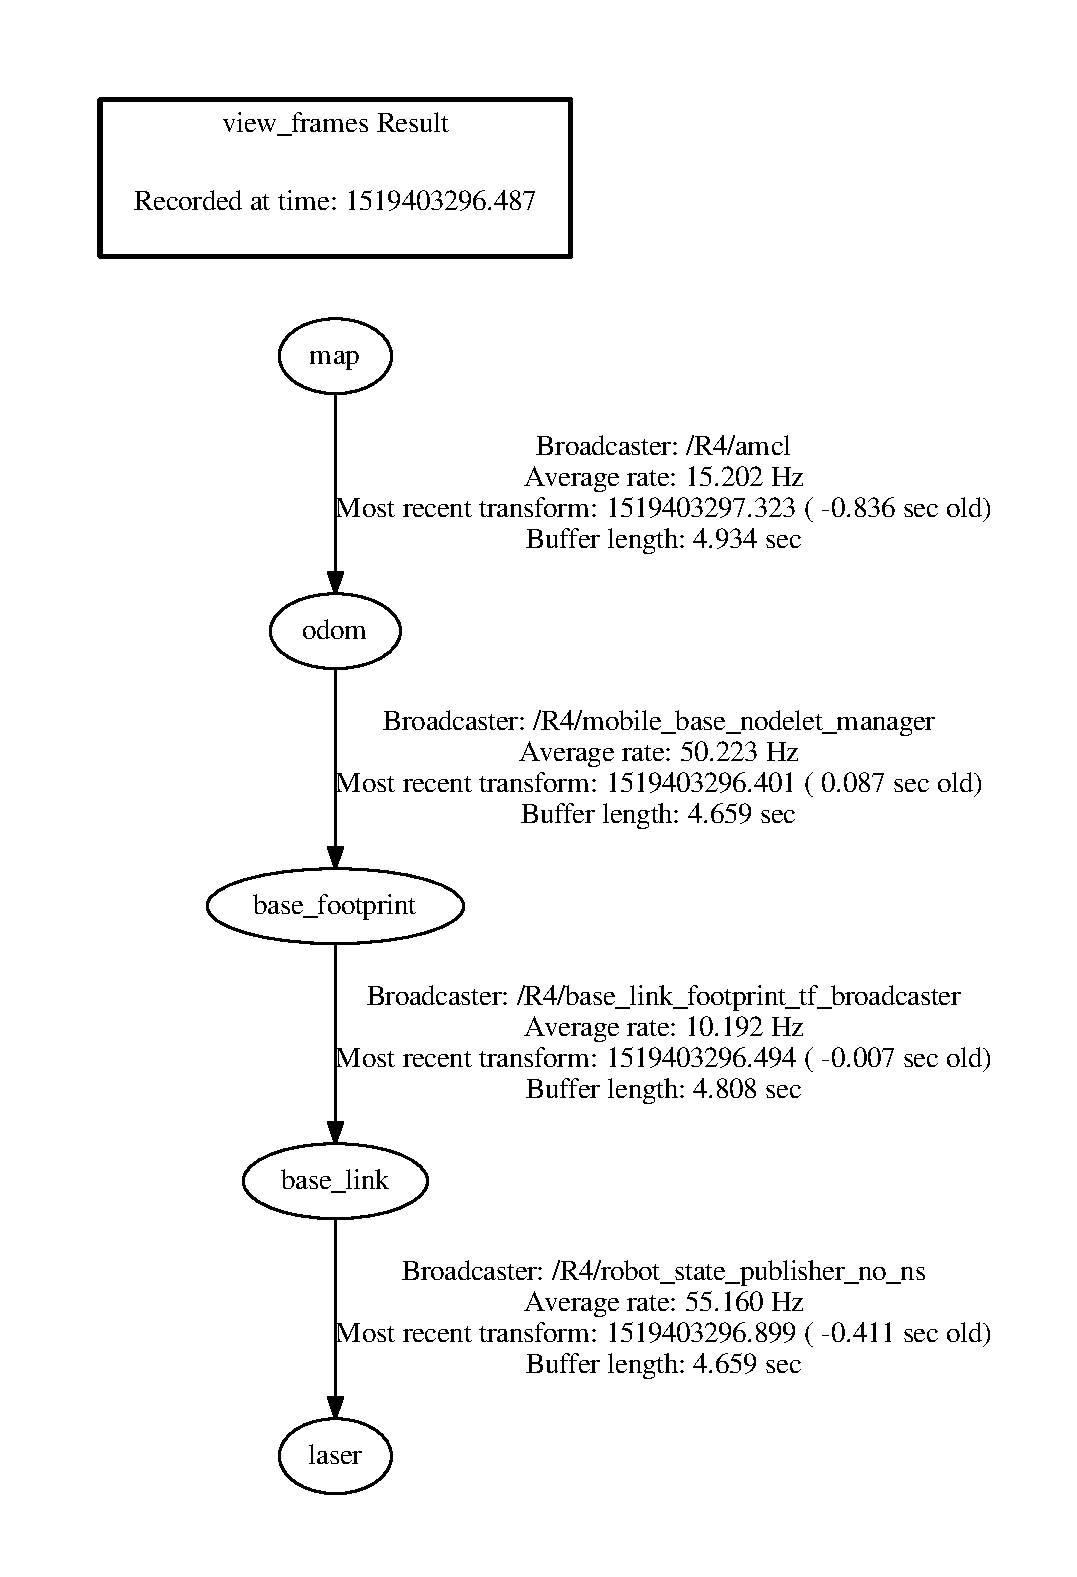
\includegraphics[width=0.4\linewidth, trim={3.5cm 1cm 1cm 5cm},clip]{img/TF_Tree_no_NS.pdf}
\caption{Transformationsbaum von Roboter 4}
\end{figure}
An dieser Stelle sei auf das ROS-Werkzeug \lstinline{tf}{} hingewiesen, das es ermöglicht mittels dem Befehl
\begin{lstlisting}
rosrun tf view_frames
\end{lstlisting}
Grafiken wie die obige zu generieren, wodurch die Fehlerfindung erleichtert wird. In dem aktuellen Transformationsbaum wird zuerst von \lstinline{map}{} nach \lstinline{odom}{} transformiert, wofür der AMCL-Knoten verantwortlich ist. Anschließend veröffentlicht der Knoten \lstinline{mobile_base_nodelet_manager}{} eine Transformation von \lstinline{odom}{} zu \lstinline{base_footprint}{}. Von \lstinline{base_footprint}{} wird wiederum in \lstinline{base_link}{} überführt. Veröffentlicht wird diese Transformation von \lstinline{base_link_footprint_tf_broadcaster}{}. Zuletzt erfolgt die Transformation von \lstinline{base_link}{} zu \lstinline{laser}{}, wofür der Knoten \lstinline{robot_state_publisher} \lstinline{_no_ns}{} zuständig ist. In dem Bezugssystem \lstinline{laser}{} werden die Daten des Laserscanners interpretiert. Bei \lstinline{base_footprint}{} und \lstinline{base_link}{} handelt es sich jeweils um körperfeste Bezugssysteme des Roboters, deren relative Ausrichtung zueinander konstant ist.

Die Knoten \lstinline{base_link_footprint_tf_broadcaster}{} und \lstinline{robot_state_}  \lstinline{publisher_no_ns}{} werden jeweils über das Slave-Skript gestartet; \lstinline{mobile_base_}{} \lstinline{nodelet_manager}{} und \lstinline{amcl}{} von der Master-Datei aus.

Ein Ansatz, um die Namenskonflikte aufzulösen, besteht darin, den Parameter \lstinline{tf_prefix}{} zu nutzen, womit ähnlich zum \lstinline{group}{}-Tag Präfixe an die Bezugssysteme der Roboter angefügt werden können.



\chapter{Ausblick und Fazit}
Im Rahmen der vorliegenden Arbeit wurde das Funktionsprinzip des ROS-Navigation-Stack erläutert und anhand von drei Experimenten bewiesen. Im ersten wurden die Grundfunktionen wie die Planung und Verfolgung des globalen Pfades nachgewiesen. Das zweite Experimente diente zur Illustration der Hindernisdetektion und der Planung bzw. Ausführung eines Ausweichmanövers. Zuletzt wurde das Konzept der Lokalisierung anhand eines dritten Experiments bewiesen, indem nur eine ungenaue Positionsschätzung bekannt war. Hier hat der Roboter innerhalb kurzer Zeit eine sichere und präzise Schätzung seiner Position erarbeitet, womit die Fähigkeit der Lokalisierung bewiesen wurde. Insofern wurden sämtliche Anforderungen an die Navigation erfüllt.


Allerdings wurde in diesen Experimenten nur die Navigation eines einzelnen Roboters untersucht. Das Ergebnis nicht auf die parallele Navigation mehrerer Roboter übertragen werden. Der Grund hierfür liegt in den Namenskonflikten der ROS-Transformationen zwischen den Robotern, die nicht vollständig aufgelöst werden konnten. In dieser Arbeit wurde versucht, mittels des ROS-Parameter \lstinline{tf_prefix}{} den Transformationen der verschiedenen Robotern Namensräume zuzuweisen, wodurch eine klare Trennung erfolgt. Allerdings hat dieser Schritt nicht die erwarteten Ergebnisse geliefert. Die exakten Ursachen des Fehlverhalten konnten in dieser Arbeit nicht geklärt werden.

Hieraus resultiert auch das offensichtliche Ziel für eine Folgearbeit: Es muss ein Konzept entwickelt werden, um die Namenskonflikte unter ROS aufzulösen.

Da die Roboter sich gegenseitig als Hindernisse wahrnehmen und somit in ihrer Pfadplanung beachten, ist zu erwarten, dass das hier vorgestellte Konzept auch bei der simultanen Navigation mehrerer Roboter funktioniert. Eine gekoppelte Navigation der Roboter sollte nicht erforderlich sein.

\begin{thebibliography}{999}\addcontentsline{toc}{chapter}{Literaturverzeichnis}%
%-----------------------------------------------------------------------%
%Name, Vorname: "Title: Untertitel", Auflage(ab 2.), Ort Jahr, Verlag
%-----------------------------------------------------------------------%
\bibitem{ProbRob} Sebastian, Thrun; Wolfram, Burgard; Dieter Fox: \glqq Probabilistic Robotics\grqq , 1. Auflage, Massachusetts Institute of Technology 2006, MIT Press
%-----------------------------------------------------------------------%
\bibitem{PlanAlgo} LaValle, Steven M. \glqq Planning Algorithms\grqq , 1. Auflage, Cambridge 2006, Cambridge University Press
%-----------------------------------------------------------------------%
\bibitem{SecRef1} Pearl, J. \glqq Heuristics\grqq , Addison-Wesley, 1984
%-----------------------------------------------------------------------%
\bibitem{SecRef2} Fikes, R. E.; Nilsson, N. J.  \glqq STRIPS: A new approach to the application of theorem proving.\grqq Artificial Intelligence Journal, 1971
%-----------------------------------------------------------------------%




\end{thebibliography}


\end{document}
